\documentclass[german,report]{i1thesis}
\usepackage{float}
\usepackage{pgf-pie}
\usepackage{pgfplots}
\pgfplotsset{compat=1.17}
\usepackage{tikz}
\usepackage{graphicx}
\usepackage{geometry}
\usepackage{amsmath}
\usepackage{tabularx}
\usepackage{longtable}
\usepackage{booktabs}
\usepackage{adjustbox}
\usepackage{makecell}

\raggedbottom

\def\theauthor{Felix Berger, B. Sc.}
\def\theadvisor{Lydia Weinberger, M. Sc. und Katharina Schiller, M. Sc.}
\def\theexaminer{Prof. Dr.-Ing. Michael Tielemann}

\def\thetitle{Erstellung von Personas für eine Sicherheits-Awareness-Kampagne an der FAU}

\def\theplace{Erlangen}
\def\thedate{\today}

\begin{document}

\makethetitle

\newpage

\section*{Abstrakt}
Informationssicherheit ist an großen Institutionen wie der Friedrich-Alexander-Universität Erlangen-Nürnberg (FAU) von zentraler Bedeutung, da Studierende und Mitarbeitende täglich mit sensiblen Daten umgehen und vielfältigen Bedrohungen, etwa Phishing-Angriffen, ausgesetzt sind. Menschliche Fehler spielen hierbei eine wesentliche Rolle, wobei rund 88\% der IT-Sicherheitsvorfälle auf solche Fehler zurückzuführen sind \cite{sebastian2021rethinking}. Dies macht den Menschen häufig zum schwächsten Glied im Sicherheitsgefüge. Ausgehend von dieser Problematik entwickelt die vorliegende Arbeit ein Konzept für eine Awareness-Kampagne an der FAU, um durch menschliches Fehlverhalten entstehende Sicherheitslücken gezielt zu adressieren.

Eine umfassende Umfrage unter den fünf Fakultäten bildet die Grundlage für fakultätsspezifische Personas, die die Informationssicherheitsgewohnheiten und Herausforderungen der Studierenden widerspiegeln. Die Umfrage deckte Themen wie VPN-Nutzung, Passwortverwaltung, Datensicherung, Zwei-Faktor-Authentifizierung, E-Mail-Verschlüsselung, Phishing-Erkennung und WLAN-Sicherung ab und umfasste allgemeine Fragen zum Sicherheitsbewusstsein und zu persönlichen Einstellungen bezüglich der Informationssicherheit. Die Ergebnisse wurden analysiert, um ein detailliertes Bild der aktuellen Sicherheitsgewohnheiten und -herausforderungen zu gewinnen.

Auf Basis dieser Analyse formuliert die Arbeit konkrete Empfehlungen zur Verbesserung des Sicherheitsbewusstseins, darunter der Einsatz von automatisierten Backups und Passwort-Managern. Durch fakultätsspezifische Maßnahmen und zielgruppengerechte Inhalte soll eine nachhaltige Stärkung der Informationssicherheitsgewohnheiten erreicht werden. Abschließend werden die Limitationen der Arbeit und Perspektiven für zukünftige Kampagnen skizziert.
\newpage

\maketoc

\newpage

\section{Einleitung}
\label{sec:introduction}

In der heutigen digital vernetzten Welt ist die Informationssicherheit ein zentrales Anliegen, besonders an akademischen Institutionen wie der FAU, wo die Digitalisierung von Forschung und Lehre stetig voranschreitet. Angesichts dieser Entwicklung setzt sich die FAU das Ziel, eine Kultur der Sicherheitsbewusstheit innerhalb ihrer vielfältigen Studierendenschaft zu fördern. Ein besonderes Augenmerk liegt dabei auf der Heterogenität der Studierenden, die in ihren Studienfächern, dem technischen Verständnis und dem Bewusstsein für Informationssicherheit stark variieren.\\
\\
In der Cybersicherheitsforschung wird häufig betont, dass der Mensch als schwächstes Glied in der Sicherheitskette gilt, da der Großteil der Sicherheitsvorfälle durch menschliche Fehler verursacht wird \cite{sebastian2021rethinking}. Vor diesem Hintergrund erkennt die FAU die Notwendigkeit, Personas auf Basis wissenschaftlicher Standards zu erstellen, um die Studierenden gezielt zu sensibilisieren.\\
\\
Diese Personas repräsentieren die breite Diversität der Studierendenschaft, welche sich über fünf Fakultäten erstreckt. Die Entwicklung dieser Personas erfolgt durch einen Onlinefragebogen, um ein Verständnis für die verschiedenen Bedürfnisse, Einstellungen und Verhaltensweisen in Bezug auf Informationssicherheit zu gewinnen. Sie dienen als Grundlage für die maßgeschneiderte Gestaltung der Awareness-Kampagne, mit dem Ziel, die Studierenden effektiv zu erreichen und zu sensibilisieren. Dadurch soll sichergestellt werden, dass die Kampagne nicht nur auf ein breites Bewusstsein abzielt, sondern auch das notwendige Wissen und die Werkzeuge vermittelt, um die Studierenden im Umgang mit den Risiken der digitalen Welt zu befähigen.

\subsection{Forschungsfragen}

Die vorliegende Arbeit untersucht folgende Forschungsfragen:

\begin{enumerate}
    \item Wie variieren Wahrnehmung und Verhalten bezüglich Informationssicherheit in unterschiedlichen Studierendengruppen?
    \item Welche spezifischen Sicherheitsbedürfnisse und -kenntnisse existieren in den verschiedenen Fakultäten?
    \item Wie kann auf Basis der ermittelten Sicherheitsbedürfnisse und -kenntnisse eine Awareness-Kampagne gestaltet werden?
\end{enumerate}

\subsection{Beiträge der Arbeit}

Diese Arbeit trägt in mehreren Bereichen zur Untersuchung des IT-Verhaltens und der von Studierenden getroffenen Sicherheitsvorkehrungen in diesem Bereich bei:

\begin{itemize}
    \item \textbf{Empirische Analyse des IT-Verhaltens:} Die Untersuchung liefert unter anderem Einblicke in das Nutzungsverhalten von Studierenden hinsichtlich Betriebssystemen, VPN-Diensten und der Passwortverwaltung.
    
    \item \textbf{Identifizierung von Hindernissen in der Informationssicherheit:} Die Arbeit untersucht zudem, welche Barrieren Studierende daran hindern, ihre Informationssicherheit zu verbessern und aufrecht zu erhalten.
    
    \item \textbf{Sicherheitsvorkehrungen der Studierenden:} Es werden die kürzlich unternommenen Anstrengungen zur Informationssicherheit erhoben, indem die von den Studierenden in den letzten vier Wochen getroffenen Sicherheitsmaßnahmen erfasst werden.
    
    \item \textbf{Wahrnehmung von Informationssicherheit:} Diese Arbeit zeigt auf, wie Studierende Informationssicherheit wahrnehmen und welchen Wissensstand sie zu dem Thema aufweisen.
    
    \item \textbf{Hilfesuche bei technischen Problemen:} Es wird untersucht, wie Studierende bei technischen Problemen Unterstützung suchen.
    
    \item \textbf{Erstellung von Personas:} Auf Basis der Umfragedaten werden Personas erstellt, um unterschiedliche Studierendengruppen und deren IT-Verhalten und Bedürfnisse zu charakterisieren.
    
    \item \textbf{Praxisorientierte Empfehlungen:} Auf Basis der erhobenen Daten werden Empfehlungen zur Durchführung einer Awareness-Kampagne an der FAU gegeben.
\end{itemize}

\subsection{Struktur der Arbeit}
\label{sec:outline}

Die vorliegende Arbeit ist in acht Hauptkapitel unterteilt, um eine klare und nachvollziehbare Darstellung der Forschungsziele, Methodologie und Ergebnisse zu gewährleisten.

Im ersten Kapitel wird die Einleitung präsentiert, die den thematischen Rahmen der Arbeit absteckt. Es enthält die Definition der Forschungsfragen sowie die Darstellung der wesentlichen Beiträge der Arbeit. Ziel ist es, den Lesenden einen Überblick über die Motivation und Zielsetzung der Untersuchung zu geben.

Das zweite Kapitel beschreibt die theoretische Grundlage für das Verständnis der Arbeit. Zunächst werden grundlegende Konzepte wie Personas erläutert, gefolgt von einer Betrachtung des wissenschaftlichen Umfragedesigns. Hierbei werden Aspekte wie das Verständnis der gestellten Fragen, die Antwortalternativen, der Kontext der Fragen und die Operationalisierung latenter Konstrukte beschrieben. Abschließend werden die Qualitätskriterien wissenschaftlicher Umfragen wie Validität, Reliabilität und Objektivität thematisiert.
Im Anschluss an diese theoretischen Grundlagen werden konkrete Beispiele aufgeführt, die zeigen, wie diese Prinzipien bei der Überarbeitung und Optimierung des Fragebogens angewendet wurden, um die wissenschaftliche Aussagekraft der erhobenen Daten zu verbessern.

In Kapitel 3 erfolgt eine Analyse der bestehenden Literatur und verwandter Arbeiten. Es wird ein Überblick über Kampagnen zur Sensibilisierung für Informationssicherheit, visuelle Ansätze und Schulungsansätze gegeben. Zudem wird die Relevanz von Phishing-Bewusstsein im akademischen Umfeld und am Arbeitsplatz erörtert, sowie der soziale Einfluss auf die Sicherheitsempfindlichkeit. Abschließend werden die Herausforderungen bei Kampagnen zur Sensibilisierung für Informationssicherheit beleuchtet.

Das vierte Kapitel beschreibt die Methodologie der durchgeführten Untersuchung. Es wird erläutert, wie die Rekrutierung der Teilnehmenden erfolgte und welche Analysemethoden für die Datenauswertung verwendet wurden. Der methodische Ansatz wird hierbei so beschrieben, dass er eine Reproduzierbarkeit der Ergebnisse ermöglicht.

Die Ergebnisse der Umfrage werden in Kapitel 5 detailliert dargestellt. Es werden demografische Daten wie die Verteilung der Teilnehmer nach Fakultäten, Geschlecht, Alterskategorien, Familienstand und Kinderzahl präsentiert. Anschließend werden die Resultate fakultätsweise aufgegliedert, einschließlich geschlossener und offener Fragen. Ein Vergleich der Limbic Types \cite{hausel2011wissenschaftliche} der Studierenden pro Fakultät und die Analyse passender Symbole und Maskottchen für IT-Sicherheit runden dieses Kapitel ab. Schließlich wird die Entwicklung von Personas auf Basis der Umfragedaten beschrieben.

In Kapitel 6 werden konkrete Maßnahmen zur Umsetzung der Awareness-Kampagne vorgeschlagen. Es werden verschiedene Kampagnenthemen wie Backups, Software-Updates, sichere Passwortverwaltung und Zwei-Faktor-Authentifizierung behandelt. Zudem werden Themen wie die Nutzung von VPN-Diensten und die Sicherung von WLAN erläutert.

Kapitel 7 beschreibt die Limitationen der Arbeit, insbesondere hinsichtlich der Generalisierbarkeit der Ergebnisse und potenzieller methodischer Einschränkungen.

Das abschließende Kapitel fasst die wichtigsten Erkenntnisse der Arbeit zusammen und gibt einen Ausblick auf mögliche zukünftige Forschungsarbeiten.

\section{Hintergrund} 
\label{sec:background}

Das folgende Kapitel bietet einen Überblick über die theoretische und praktische Relevanz von Personas, um das Verständnis und die Bedeutung dieser Konzepte zu klären. Anschließend liegt der Schwerpunkt auf der Identifizierung und Anwendung wissenschaftlicher Methoden sowie auf Qualitätsstandards, die für das Design von Umfragen relevant sind. Des Weiteren werden die Qualitätskriterien qualitativer Umfragen definiert. Die gewonnenen Erkenntnisse dienen als Grundlage für die notwendige Überarbeitung und Optimierung des bestehenden Fragebogens, um dessen wissenschaftliche Aussagekraft zu verbessern.

\subsection{Personas}
\label{sec:personas}
Der folgende Abschnitt widmet sich der eingehenden Betrachtung und Anwendung von Personas innerhalb der wissenschaftlichen Forschung. Durch eine Hintergrundanalyse werden zunächst die Grundlagen und die Bedeutung von Personas auf die Sicherheits-Awareness-Kampagne der FAU erörtert.\\
\\
Personas stellen, wie Schweibenz et al. \cite{Schweibenz} beschreibt, fiktive, archetypische Charaktere dar, die die realen Nutzer repräsentieren. Sie fungieren als sorgfältig ausgearbeitete Konstrukte und dienen als Stellvertreter für die tatsächlichen Zielgruppen, indem sie deren wesentliche Anforderungen, Bedürfnisse und Zielsetzungen einfangen. Bei ihrer Entwicklung wird mit hoher Präzision und logischer Kohärenz vorgegangen, um sicherzustellen, dass sie die Erwartungen und Ziele der zukünftigen Anwender widerspiegeln.\\
Die Ermittlung der Personas ist durch den gezielten Einsatz einer Umfrage vorgesehen.\\
\\
Diese methodische und zielgerichtete Erstellung von Personas dient als das Herzstück der Sicherheits-Awareness-Kampagne der FAU, mit dem primären Ziel, effektiv die Studierenden von fünf ausgewählten Fakultäten zu erreichen und zu sensibilisieren. Der Einsatz dieser Personas ermöglicht eine maßgeschneiderte und tiefgehende Ansprache der Studierenden, indem die Kampagne direkt auf die spezifischen Bedürfnisse und Herausforderungen der Zielgruppe eingeht. Dieser Ansatz stellt nicht nur ein umfassendes Bewusstsein für Sicherheitsfragen sicher, sondern gewährleistet auch, dass jeder Studierende mit dem erforderlichen Wissen und den nötigen Werkzeugen ausgestattet wird, um sich in der digitalen Welt sicher zu bewegen. Indem die Personas als zentrales Element in die Gestaltung der Kampagne integriert werden, schaffen wir eine solide Basis für eine wirkungsvolle Sensibilisierung und Befähigung der Studierenden im Umgang mit digitalen Sicherheitsrisiken.

\subsection{Wissenschaftliches Umfragedesign}
\label{sec:survey_design}

Der nachfolgende Abschnitt präsentiert eine Hintergrundanalyse mit dem Ziel, wissenschaftliche Methodiken und Qualitätskriterien für Umfragedesigns zu identifizieren, die sowohl in quantitativen als auch in qualitativen Forschungskontexten Anwendung finden. Diese Erkenntnisse werden anschließend genutzt, um den bestehenden Fragebogen entsprechend zu verbessern und zu erweitern.\\
\\
Selbstberichte zu Verhaltensweisen und Einstellungen sind signifikant von den Charakteristika des eingesetzten Forschungsinstruments beeinflusst. Dazu zählen Aspekte wie die Art der Fragestellung, das Format und der Kontext, in dem die Fragen gestellt werden \cite{Schwarz1999}. Das Ziel dieses Abschnitts besteht darin, einen umfassenden Überblick über die wissenschaftlichen Erkenntnisse zu den Prozessen zu geben, die nicht nur Selbstberichten, sondern auch anderen Erhebungsmethoden zugrunde liegen. Dies soll die Basis für die notwendige Überarbeitung des bereits vorhandenen Fragebogens bilden. Durch ein tieferes Verständnis dieser Dynamiken können präzisere und aussagekräftigere Daten erhoben werden, was wiederum die Qualität und Validität der Forschungsergebnisse erhöht.

\subsubsection{Verständnis der gestellten Frage}

Das semantische Verständnis einer Frage involviert die Identifikation von Worten, das Abrufen lexikalischer Informationen aus dem semantischen Gedächtnis und den Aufbau einer Bedeutung der Äußerung, die durch ihren Kontext eingeschränkt wird. Forschende werden angehalten, einfache Fragen zu formulieren und unbekannte oder mehrdeutige Begriffe zu vermeiden. Doch das Verständnis der Wörter allein reicht nicht aus, um eine Frage zu beantworten. Befragte müssen auch Inferenzen über die Intention des Fragestellers anstellen, um die pragmatische Bedeutung der Frage zu erschließen \cite{Schwarz1999}. Lucas und Baird \cite{LucasBaird2006} ergänzen, dass das Frageverständnis durch subtile Änderungen in der Frageformulierung, der Fragefolge und den Antwortoptionen beeinflusst werden kann, was wiederum die gegebenen Antworten erheblich verändert.

\subsubsection{Die Antwortalternativen}

Bei offenen Antwortformaten müssen Befragte selbst bestimmen, welche Aktivitäten für den Forschenden von Interesse sein könnten. Dies folgt der Maxime der Quantität, wonach Befragte dazu neigen, Aktivitäten wegzulassen, von denen sie annehmen, dass der Forschende sie ohnehin kennt oder als selbstverständlich betrachtet. Werden Befragten hingegen eine Liste von Aktivitäten vorgelegt, sind sie wahrscheinlich geneigt, diese zu bestätigen \cite{Schwarz1999}. Lucas und Baird \cite{LucasBaird2006} weisen darauf hin, dass die Art der Antwortalternativen und der Zeitrahmen einer Frage die Interpretation und damit die Antworten der Befragten signifikant beeinflussen können.

\subsubsection{Der Kontext der Frage}

Ein wichtiger, oft übersehener Kontextfaktor, der die Interpretation der Frage durch die Befragten beeinflussen kann, sind Hinweise auf die Zugehörigkeit des Forschenden. Die Normen der Gesprächsführung erfordern, dass Sprecher Informationen bereitstellen, die für den Fragesteller von Interesse sind, was Inferenzen über das wahrscheinliche Interesse des Forschenden erfordert \cite{Schwarz1999}. Lucas und Baird \cite{LucasBaird2006} betonen, dass die Genauigkeit und Validität von Selbstberichten oft beeindruckend ist, trotz der Vielzahl von Problemen, die bei der Erstellung eines Selbstberichtsurteils auftreten können. Sie legen dar, dass Abweichungen zwischen Selbstberichten und anderen Erhebungsmethoden häufig nicht auf Irrtümer der Befragten zurückgehen, sondern vielmehr darauf hindeuten, dass Selbstberichte bedeutende Ereignisse, prognostizieren können.

\subsubsection{Operationalisierung latenter Konstrukte}

Die Operationalisierung ist essentiell in der empirischen Forschung, insbesondere bei der Messung theoretischer Konzepte wie Vertrauen oder dem sozialen Status, die als latente Konstrukte betrachtet werden. Solche Konstrukte sind nicht direkt beobachtbar und stellen daher eine signifikante Herausforderung in der Forschung dar. Um diese Konstrukte messbar zu machen, müssen präzise Definitionen und relevante Indikatoren entwickelt werden. Indikatoren dienen dabei als messbare Repräsentanten des latenten Konstrukts und sollten durch sorgfältig ausgewählte Fragen im Umfragedesign reflektiert werden\cite{Tausendpfund2018}.  \\ 
\\
Die Verbindung zwischen theoretischen Begriffen und ihren Indikatoren erfolgt über Korrespondenzregeln. Diese Regeln stellen die methodische Brücke zwischen dem nicht direkt beobachtbaren Konzept und dem beobachtbaren Indikator dar \cite{Tausendpfund2018}. \\
\\
Die Auswahl von Indikatoren wie Bildung, berufliche Stellung und Einkommen zur Operationalisierung des sozialen Status zeigt, dass verschiedene Indikatoren unterschiedliche Aspekte eines Konzepts beleuchten können und nicht immer identische Ergebnisse liefern. Dies bestätigt, dass die Korrespondenzregel im Grunde eine Hypothese über den Zusammenhang zwischen einem Indikator und einem theoretischen Konzept darstellt. Es ist möglich, dass eine Korrespondenzregel fehlerhaft ist, was bedeutet, dass der gewählte Indikator keinen validen Rückschluss auf das zugrundeliegende Konzept zulässt \cite{Tausendpfund2018}.\\
\\
Die vorangehenden Abschnitte haben die komplexen Aspekte beleuchtet, die bei der Gestaltung von Forschungsinstrumenten und der Interpretation von Daten aus Selbstberichten beachtet werden müssen. Sie unterstreichen, wie essenziell ein tiefgreifendes Verständnis dieser Dynamiken für die Sicherstellung der Validität und Reliabilität in der Forschung ist.

\subsection{Qualitätskriterien wissenschaftlicher Umfragen}

Dieser Abschnitt konzentriert sich auf die entscheidenden Qualitätskriterien qualitativer und quantitativer Studien: Validität, Reliabilität und Objektivität. Diese Begriffe sind essenziell für die Entwicklung und Beurteilung wissenschaftlicher Messinstrumente, da sie Aufschluss darüber geben, wie verlässlich die erhobenen Daten die Zielmerkmale oder Konstrukte erfassen.\\
\\
Die Qualität qualitativer Umfragen wird maßgeblich durch zwei zentrale Kriterien bestimmt: Validität und Reliabilität \cite{Bolarinwa2015}. Diese Konzepte sind entscheidend für die Entwicklung und Bewertung wissenschaftlicher Messinstrumente, da sie Aufschluss darüber geben, inwieweit die erhobenen Daten verlässlich sind und die beabsichtigten Merkmale oder Konstrukte erfassen. In diesem Kontext wird das Kriterium der Objektivität in Verbindung mit qualitativen Forschungsmethoden nicht weiter betrachtet. Der Grund dafür liegt in der spezifischen Natur qualitativer Forschung. Objektivität, die oft als die Unabhängigkeit der Messergebnisse von der Person des Forschenden definiert wird, findet in der qualitativen Forschung seltener Anwendung, da hier die interpretative Analyse und das tiefe Verständnis der Daten im Vordergrund stehen \cite{Flick2020}. 

\subsubsection{Validität}

Validität bezeichnet das Ausmaß, in dem ein Messinstrument tatsächlich das misst, was es zu messen vorgibt. Es gibt verschiedene Arten von Validität, welche sich in zwei übergeordnete Kategorien einteilen: interne und externe Validität. Die interne Validität bezieht sich darauf, wie genau die aus der Forschung gewonnenen Messwerte tatsächlich das quantifizieren, was sie messen sollen. Die externe Validität hingegen beschreibt, wie präzise die aus der Stichprobe gewonnenen Messwerte die Referenzpopulation repräsentieren, aus der die Stichprobe entnommen wurde \cite{Bolarinwa2015}. 

\subsubsection{Reliabilität}

Eine grundlegende Anforderung an ein psychometrisches Instrument ist die Zuverlässigkeit (Reliabilität). Dies bezieht sich auf die Notwendigkeit, dass ein Fragebogen konsistente Ergebnisse liefert, wenn er wiederholt unter denselben Bedingungen mit denselben Teilnehmern verwendet wird, und somit relativ unbeeinflusst von Messfehlern ist. Der gebräuchlichste Index dafür ist der Alpha Koeffizient \cite{Cronbach1951}. Bei der Anwendung auf Fragebögen ermöglicht diese Statistik die Beurteilung der internen Konsistenz eines Fragebogens, indem sie die Varianz der Gesamtscores mit den Varianzen der Scores für jedes einzelne Item vergleicht. Dieser Prozess schätzt die Reliabilität des Fragebogens, indem er misst, inwiefern alle Items konsequent dasselbe Konstrukt erfassen und folglich zur Gesamtzuverlässigkeit des Fragebogens beitragen \cite{BRAUN20121}.\\

\subsubsection{Objektivität}

Objektivität in der quantitativen Forschung erfordert, dass Sachverhalte möglichst neutral und unvoreingenommen präsentiert werden, wobei ein sachlicher Sprachstil verwendet wird. Das Ziel ist, dass die Gültigkeit der Forschungsergebnisse weitgehend unabhängig von den persönlichen Eigenschaften des Forschers oder des Beobachters bestehen bleibt. Obwohl vollständige Objektivität oft schwer zu erreichen ist, da Wahrnehmungen tendenziell subjektiv sind oder bestenfalls als intersubjektiv angesehen werden, wenn sie durch die Beobachtungen mehrerer Personen bestätigt werden, bleibt die Forderung bestehen, Sachverhalte unverfälscht und aus verschiedenen Perspektiven zu betrachten, um eine umfassende und korrekte Darstellung zu ermöglichen \cite{Heesen2014}.\\
\\
Durch die Kombination wissenschaftlicher Methoden und praxisnaher Erkenntnisse aus dem Marketing lassen sich Fragestellungen fundiert weiterentwickeln und in eine wissenschaftlich solide Form überführen. Diese Synergie ermöglicht nicht nur die Erweiterung und Verbesserung des Fragebogens, sondern steigert auch seine wissenschaftliche Strenge. So wird die Validität, Reliabilität und Objektivität der aus den Umfragen gewonnenen Daten gesichert, und fundierte Erkenntnisse aus beiden Bereichen fließen zielführend zusammen. Indem die Fragen auf wissenschaftlichen Methoden und anerkannten Qualitätskriterien basieren, wird gewährleistet, dass die erhobenen Daten verlässlich sind und die beabsichtigten Merkmale oder Konstrukte präzise erfassen.
Die Berücksichtigung von Validität und Reliabilität in der Konzeption und Durchführung von Umfragen bildet somit die Grundlage für die Erstellung von Personas, die über eine rein marketingorientierte Anwendung hinausgehen und einen wertvollen Beitrag zur wissenschaftlichen Forschung leisten.
Nachfolgend werden konkrete Beispiele für die Umsetzung dieser Prinzipien im Fragebogendesign dargestellt, die zeigen, wie durch gezielte Anpassungen eine höhere Datenqualität und Aussagekraft erreicht werden können.

\subsection{Beispiele der Verbesserung des Fragebogens}

Um die wissenschaftlichen Erkenntnisse des Umfragedesigns in die Praxis umzusetzen, wurden u.\,a. die folgenden Änderungen am Fragebogen vorgenommen. Diese basieren auf den Erkenntnissen zur Fragengestaltung, den Antwortalternativen, dem Kontext der Fragen sowie der Operationalisierung latenter Konstrukte (siehe Abschnitt~\ref{sec:survey_design}). Die Anpassungen stellen sicher, dass die Qualitätskriterien Validität, Reliabilität und Objektivität eingehalten werden.

\subsubsection{Sicherheitsvorkehrungen}

Diese Frage wurde ausgewählt, da sie für das Verständnis der Sicherheitspraktiken der Zielgruppe essenziell ist. Die Überarbeitung berücksichtigt Aspekte des Frageverständnisses und der Antwortalternativen.

\paragraph{Originalfrage:}

Welche der folgenden Sicherheitsvorkehrungen hast du in den letzten 4 Wochen getroffen?

\begin{itemize}
    \item Sicherheits-Backup meiner Daten erstellt
    \item System- oder Softwareupdates auf meinem PC/Laptop durchgeführt
    \item E-Mail-Sicherheitszertifikat erstellt
    \item E-Mail-Sicherheitszertifikat für die Verschlüsselung oder Signatur von E-Mails genutzt
\end{itemize}

\paragraph{Überarbeitete Frage:}

Welche der folgenden Sicherheitsvorkehrungen hast du in den letzten 4 Wochen getroffen?

\begin{itemize}
    \item Sicherheits-Backup meiner Daten erstellt
    \item System- oder Softwareupdates auf meinem PC/Laptop durchgeführt
    \item E-Mail-Sicherheitszertifikat erstellt
    \item E-Mail-Sicherheitszertifikat für die Verschlüsselung oder Signatur von E-Mails genutzt
    \item Antivirensoftware installiert oder aktualisiert
    \item Zwei-Faktor-Authentifizierung (2FA) für Online-Konten aktiviert
    \item Zwei-Faktor-Authentifizierung (2FA) für Online-Konten genutzt
    \item Phishing-E-Mails erkannt
    \item Phishing-E-Mails gemeldet
    \item WLAN-Verbindung gesichert (z.\,B. durch Änderung des Standard-Passworts)
    \item Keine dieser Vorkehrungen
    \item Sonstiges
\end{itemize}

\paragraph{Wissenschaftliches Umfragedesign:}

Die Überarbeitung der Frage basiert auf den in Abschnitt~\ref{sec:survey_design} dargestellten wissenschaftlichen Erkenntnissen. Gemäß \citet{Schwarz1999} beeinflussen die Art der Fragestellung und die Antwortalternativen die Antworten der Befragten maßgeblich. Indem wir die Antwortoptionen erweitern, berücksichtigen wir die Maxime der Quantität und vermeiden, dass Befragte wichtige Aktivitäten weglassen, die sie für selbstverständlich halten könnten.

Die Aufnahme weiterer relevanter Sicherheitsmaßnahmen erhöht die \textbf{Validität} der Frage, da sie ein umfassenderes Spektrum an Praktiken abdeckt. Laut \citet{LucasBaird2006} können subtile Änderungen in der Frageformulierung und den Antwortoptionen die Interpretation der Befragten beeinflussen. Durch präzise und klare Formulierungen fördern wir das Verständnis der Frage und reduzieren Missverständnisse, was die \textbf{Reliabilität} erhöht.

Die neutrale Gestaltung der Frage und Antwortoptionen gewährleistet die \textbf{Objektivität} der Datenerhebung. Zudem ermöglicht die Option "Keine dieser Vorkehrungen" den Befragten, ehrlich zu antworten, ohne beeinflusst zu werden, was den Empfehlungen zur ethischen Gestaltung von Fragen entspricht.

\subsubsection{VPN-Nutzung}

Diese Frage wurde angepasst, um differenzierte Nutzungskontexte von VPN-Diensten abzubilden. Die Änderungen berücksichtigen den Kontext der Frage und erweitern die Operationalisierung latenter Konstrukte.

\paragraph{Originalfrage:}

Hast du bereits Erfahrungen mit der Nutzung eines VPN-Dienstes gemacht?

\begin{itemize}
    \item Ja
    \item Nein
\end{itemize}

\paragraph{Überarbeitete Frage:}

Hast du bereits Erfahrungen mit der Nutzung eines VPN-Dienstes gemacht? Wähle alle zutreffenden Optionen.

\begin{itemize}
    \item Privat genutzt
    \item Im Arbeitsumfeld genutzt
    \item FAU-Dienst genutzt
    \item Weiß ich nicht
    \item Nein
\end{itemize}

\paragraph{Wissenschaftliches Umfragedesign:}

Gemäß den Erkenntnissen zur \textbf{Operationalisierung latenter Konstrukte} \cite{Tausendpfund2018} ist es wichtig, theoretische Konzepte präzise zu definieren und durch relevante Indikatoren messbar zu machen. Die Erweiterung der Antwortoptionen ermöglicht es, das Konstrukt der VPN-Nutzung in unterschiedlichen Kontexten genauer zu erfassen, was die \textbf{Validität} erhöht.

Die klar definierten Antwortmöglichkeiten reduzieren laut \citet{Schwarz1999} die Notwendigkeit für Befragte, Inferenzen über die Intention des Fragestellers zu machen, was das Frageverständnis verbessert. Dies trägt zur \textbf{Reliabilität} bei, indem konsistente und vergleichbare Daten gewährleistet werden.

Die neutrale Formulierung der Antwortoptionen gewährleistet die \textbf{Objektivität}, indem keine Wertung oder Beeinflussung der Teilnehmer vorgenommen wird.

\subsubsection{Passwortspeicherung}

Diese Frage wurde angepasst, um die erhobenen Daten durch präzisere Antwortoptionen zu erweitern und eine breitere Grundlage für die Analyse von Passwortpraktiken zu schaffen.

\paragraph{Originalfrage:}

Erinnerst du dich korrekt an die Passwörter deiner zehn zuletzt genutzten Accounts?

\begin{itemize}
    \item Ich kenne alle Passwörter auswendig, ohne zu raten
    \item Ich kenne die meisten Passwörter auswendig, muss aber bei einigen raten
    \item Ich kenne einige Passwörter auswendig, muss aber bei vielen raten
    \item Ich kenne kaum oder keine Passwörter auswendig und muss meistens raten
    \item Ich speichere / notiere mir meine Passwörter
\end{itemize}

\paragraph{Überarbeitete Frage:}

Erinnerst du dich korrekt an die Passwörter deiner zehn zuletzt genutzten Accounts? Wähle die zutreffendsten Aussagen aus.

\begin{itemize}
    \item Ich kenne alle Passwörter auswendig und muss nie raten
    \item Ich kenne die meisten Passwörter, muss bei einigen aber raten
    \item Ich kenne einige Passwörter, muss bei vielen jedoch raten
    \item Ich kenne keine oder kaum Passwörter auswendig und muss fast immer raten
    \item Ich verwende Hilfsmittel wie Passwortmanager oder schriftliche Notizen
\end{itemize}

\paragraph{Wissenschaftliches Umfragedesign:}

Die Anpassung dieser Frage berücksichtigt die Erkenntnisse zur \textbf{Operationalisierung latenter Konstrukte} \cite{Tausendpfund2018}, indem sie sowohl das Erinnerungsvermögen als auch das Verhalten im Passwortmanagement erfasst. Durch die Ergänzung um die Nutzung von Hilfsmitteln wird ein umfassenderes Bild des Konstrukts gewonnen, was die \textbf{Validität} erhöht.

Gemäß \citet{LucasBaird2006} kann die Art der Antwortalternativen die Interpretation der Befragten beeinflussen. Die klar formulierten Antwortmöglichkeiten fördern das Verständnis der Frage und reduzieren die kognitive Belastung, was zur \textbf{Reliabilität} beiträgt.

Die neutrale Gestaltung der Frage und Antwortoptionen gewährleistet die \textbf{Objektivität}, indem sie den Befragten ermöglicht, ihre tatsächlichen Passwortpraktiken ohne Beeinflussung oder Wertung anzugeben.

\subsubsection{Demographische Daten}

Diese Frage wurde ausgewählt, da sie sensible Informationen abfragt und eine präzise und ethisch korrekte Gestaltung erfordert. Die Änderungen stellen sicher, dass ethische Standards eingehalten werden.

\paragraph{Originalfrage:}

Welchem Geschlecht fühlst du dich zugehörig?

\begin{itemize}
    \item Weiblich
    \item Männlich
    \item Divers
\end{itemize}

\paragraph{Überarbeitete Frage:}

Welchem Geschlecht fühlst du dich zugehörig?

\begin{itemize}
    \item Männlich
    \item Weiblich
    \item Divers
\end{itemize}

\textit{Hinweis: „Bitte beachte, dass bei der Auswahl der Option 'Divers' die Anonymität eventuell nicht vollständig gewährleistet ist.“}

\paragraph{Wissenschaftliches Umfragedesign:}

Die Frage wurde so gestaltet, dass sie alle Geschlechtsidentitäten einschließt und den Anforderungen des Datenschutzes entspricht. Der eingefügte Hinweis dient der Transparenz und wurde gemäß den Vorgaben des Datenschutzbeauftragten eingefügt, um die Teilnehmenden über mögliche Einschränkungen der Anonymität zu informieren.

Allerdings kann dieser spezifische Hinweis die \textbf{Objektivität} der Befragung beeinträchtigen, da sich Teilnehmende durch den Hinweis davon abhalten lassen könnten, die Option "Divers" zu wählen, aus Sorge um ihre Anonymität. Dies entspricht den in Abschnitt~\ref{sec:survey_design} diskutierten Kontextfaktoren, die die Interpretation der Frage beeinflussen können \cite{Schwarz1999}. Die mögliche Verzerrung der Daten kann die \textbf{Validität} beeinträchtigen, da das Konstrukt der Geschlechtsidentität nicht mehr vollständig und unverfälscht erfasst wird.

Gemäß \citet{LucasBaird2006} können Abweichungen in Selbstberichten auf den Einfluss des Fragekontextes zurückzuführen sein. Obwohl die klare und respektvolle Darstellung der Antwortoptionen grundsätzlich die \textbf{Reliabilität} fördert, muss berücksichtigt werden, dass der Hinweis potenziell dazu führen kann, dass Teilnehmende nicht ihre tatsächliche Geschlechtsidentität angeben, was die Zuverlässigkeit der Daten mindert.

\subsubsection{Fazit}

Die genannten Beispiele illustrieren, wie wissenschaftliche Erkenntnisse des Umfragedesigns (siehe Abschnitt~\ref{sec:survey_design}) und die Qualitätskriterien Validität, Reliabilität und Objektivität durch gezielte Anpassungen erfüllt werden können. Sie tragen dazu bei, die Datenqualität zu erhöhen und die Ergebnisse aussagekräftiger zu machen.


\section{Verwandte Arbeiten}
\label{sec:related_work}

\subsection{Überblick über Kampagnen zur Sensibilisierung für Informationssicherheit, visuelle Ansätze und Schulungsansätze}

Sebastian et al. \cite{sebastian2021rethinking} untersuchten, wie menschliche Fehler zur Entstehung von Cyberbedrohungen beitragen. Die Ergebnisse dieser Arbeit betonen die entscheidende Rolle menschlicher Faktoren in der Cybersicherheitsabwehr. Sie verdeutlichen, dass nicht nur Mitarbeitende als potenzielles Risiko für Sicherheitslücken gelten, sondern auch Lücken in der Sicherheitskultur und unzureichende Schulungsprogramme maßgebliche Schwachstellen darstellen. Studien zeigen, dass etwa 88\% der Sicherheitsvorfälle durch menschliche Fehler verursacht werden. Diese Schwachstellen spiegeln sich in typischen Fehlern wider, wie dem Klicken auf Phishing-E-Mails oder der dem Verbinden mit unsicheren öffentlichen Netzwerken, die häufig zu Datenlecks führen. Menschliche Fehler sind häufig eine Folge fehlender Schulung und Sicherheitskultur, was die Bedeutung gezielter Bewusstseinsschulung zur Minderung dieser Risiken unterstreicht.

Bada et al. \cite{bada2019cyber} analysierten verschiedene Ansätze zur Sensibilisierung für Cybersicherheit, die darauf abzielen, sicheres Verhalten bei Nutzern wie Mitarbeitern, Kunden und Bürgern zu fördern. Zu den untersuchten Ansätzen gehören Schulungen und Sensibilisierungskampagnen, die darauf abzielen, das Bewusstsein für Sicherheitsrisiken zu schärfen und korrektes Verhalten zu fördern. Die Autoren betonen, dass solche Programme unverzichtbar sind, um Informationen zu verbreiten, die alle Nutzer – einschließlich Manager – kennen müssen, um sicher zu handeln. Ein Ergebnis der Analyse ist, dass es nicht ausreicht, lediglich Informationen zu vermitteln; vielmehr müssen die Programme auf Verhaltensänderungen abzielen, indem sie psychologische Faktoren wie Motivation und Wahrnehmung von Risiken einbeziehen, um nachhaltig erfolgreich zu sein.

Kaya et al. \cite{kaya2023impact} untersuchten die Auswirkungen eines challenge-basierten Gamification-Programms, genannt Educhall, auf die Lernergebnisse von Studierenden in einer digitalen Lernumgebung. Educhall ist ein webbasiertes Programm, das entwickelt wurde, um durch kurze, gamifizierte Lerneinheiten die Motivation und den Lernerfolg zu steigern. Es ermöglicht Lehrkräften, Quizze zu erstellen, die Studierende absolvieren und sich gegenseitig herausfordern können, wodurch ein wettbewerbsorientiertes Umfeld geschaffen wird, das Vertrauen und Zufriedenheit fördert. Ihre Studie verglich 30 Studierende in einer Kontrollgruppe mit 30 Studierenden in einer Experimentalgruppe, die Educhall nutzten. Die Ergebnisse zeigten, dass die Experimentalgruppe eine signifikant höhere akademische Leistung und gesteigerte Motivation erreichte. Insbesondere zeigten sich höhere Werte in den Unterfaktoren Vertrauen und Zufriedenheit. Obwohl das Gamification-Programm den Fluss (Flow) der Lernenden leicht steigerte.

Al.masri \cite {almasri2018groupwork} untersuchte die Auswirkungen der Gruppenarbeitsstrategie auf die Leistungen von Studenten. Die Studie zielte darauf ab, den Zusammenhang zwischen hohen Studienleistungen und dem Lernen durch Gruppenarbeit zu erforschen. Es wurde eine deskriptive Methodik verwendet, die verschiedene Bildungsstudien und Literatur einbezog. Die Ergebnisse zeigten, dass Gruppenarbeit das Lernen und die Leistungen der Studenten signifikant verbessert und deren Fähigkeiten und Verhalten fördert. Aufgrund dieser Ergebnisse empfiehlt die Studie, Inhalte zu entwickeln, die die Ziele dieser Strategie unterstützen, und Lehrkräfte in der effektiven Umsetzung zu schulen.

Pang et al. \cite{pang2021graphicwarnings} untersuchten die Wirkung von bildlichen Gesundheitswarnungen auf die Wahrnehmung und das Verhalten der Menschen in Bezug auf Rauchen. Ihre Ergebnisse zeigten, dass solche Warnungen im Vergleich zu textbasierten Hinweisen eine stärkere Wirkung auf die Risikowahrnehmung und die Absicht zur Verhaltensänderung haben. Diese Erkenntnisse verdeutlichen, dass visuelle und emotionale Elemente in Sensibilisierungskampagnen eine effektive Methode sein können, um Aufmerksamkeit zu erregen und Verhaltensänderungen zu fördern. Solche Ansätze könnten auch in Kampagnen zur Informationssicherheit Anwendung finden, indem visuelle Elemente verwendet werden, um das Bewusstsein für Risiken zu steigern und eine sicherere Nutzung digitaler Technologien zu fördern.

\subsection{Phishing-Bewusstsein im akademischen Umfeld und am Arbeitsplatz}

Hillman et al. \cite{hillman2023evaluating} führten in ihrer Studie simulierte Phishing-Angriffe in einem großen israelischen Finanzinstitut durch, um die Effektivität von Schulungsprogrammen zur Sensibilisierung der Mitarbeiter zu bewerten. Sie beschrieben Phishing als eine Technik, bei der der Benutzer getäuscht wird, indem eine legitime Organisation vorgetäuscht wird, um sensible Daten zu erhalten. Die Studie fand heraus, dass personalisierte Phishing-Mails deutlich effektiver sind und die Wahrscheinlichkeit erhöhen, dass Mitarbeiter darauf hereinfallen. Zudem stellten sie fest, dass gezielte Schulungsprogramme die Sicherheit deutlich verbessern können. Bei einem typischen Phishing-Angriff wird eine Nachricht gesendet, die scheinbar von einer vertrauenswürdigen Organisation, wie z. B. einer Bank, stammt, um sensible Daten wie Benutzernamen und Passwörter zu stehlen.

Hudson et al. \cite{hudson2023phishing} untersuchten Phishing-Angriffe auf Bildungseinrichtungen und fanden heraus, dass diese zu den am häufigsten betroffenen Sektoren gehören. In ihrer Studie analysierten sie eine Vielzahl von Angriffen und deren Auswirkungen auf verschiedene Bildungseinrichtungen, wobei sie einen Anstieg der Angriffe und eine zunehmende Komplexität der verwendeten Methoden feststellten. Kenntnisse zur Erkennung von Phishing-Versuchen sind in akademischen und professionellen Umgebungen unerlässlich, da diese Umgebungen von einer heterogenen Benutzerschaft geprägt sind, die unterschiedlich stark mit Cybersicherheitsgefahren konfrontiert wird.

In einer Studie von Reinheimer et al. \cite{reinheimer2020investigation} wurde gezeigt, dass Sicherheitsbewusstsein und entsprechende Bildungsprogramme für unterschiedliche Benutzergruppen, wie beispielsweise Mitarbeiter in öffentlichen Verwaltungen, entscheidend sind, um Phishing-Angriffe erfolgreich zu identifizieren und abzuwehren. Die Studie belegt, dass regelmäßige Schulungen und Erinnerungen das Erkennen von Phishing-Mails erheblich verbessern und über längere Zeiträume hinweg wirksam sind, besonders in Umgebungen mit stark variierendem technischen Wissen der Benutzer.

\subsection{Sozialer Einfluss auf die Sicherheitsempfindlichkeit}

Das et al. \cite{185300} untersuchten, wie sozialer Einfluss das Sicherheitsverhalten prägt. Sie betonen, dass unser Verhalten stark von den Normen und dem Verhalten unserer Mitmenschen beeinflusst wird. Die Studie zeigt, dass soziale Prozesse wie das Beobachten von Freunden und das Lernen im sozialen Kontext eine wichtige Rolle bei der Anpassung des Sicherheitsverhaltens spielen. Sie fanden heraus, dass der soziale Beweis – also die Idee, dass Menschen dem Beispiel anderer folgen – einen großen Einfluss darauf hat, wie und ob Sicherheitsmaßnahmen angewendet werden. Außerdem legen sie nahe, dass die Sichtbarkeit von Sicherheitsmaßnahmen, wie das Nutzen von Sicherheitsfeatures durch Gleichaltrige, das Bewusstsein und die Motivation erhöht, selbst sicherheitsbewusst zu handeln.

Die Studie von Akers et al. \cite{akers1995social} in der kognitiven Psychologie untersucht die psychologischen Prozesse, die dem sozialen Einfluss zugrunde liegen. Akers et al. \cite{akers1995social} führten Experimente durch, um zu verstehen, wie soziale Normen das Verhalten von Individuen beeinflussen. Die Ergebnisse zeigen, dass Menschen dazu neigen, ihr Verhalten an den wahrgenommenen Erwartungen ihrer sozialen Gruppe auszurichten, um Akzeptanz und Zugehörigkeit zu erlangen. Dies deutet darauf hin, dass das Verhalten von Individuen stark von der sozialen Umgebung und den innerhalb dieser Gruppen bestehenden Normen geprägt ist.

Zusammengenommen deuten die Erkenntnisse aus den beschriebenen Studien darauf hin, dass die Entscheidungen und Verhaltensweisen der Menschen – insbesondere in Bezug auf die Sicherheit – in großem Maße durch sozialen Einfluss gelenkt werden. In der Tat hat frühere Forschungsarbeit \cite{yazdanmehr2020peers} auf die Rolle hingewiesen, die die soziale Dynamik bei der Erhöhung der Sicherheitsempfindlichkeit spielt. Indem das Verhalten anderer Nutzer in einer nachvollziehbaren Situation gezeigt wird, kann beispielsweise die soziale Navigation oder die Neigung der Menschen, nach Hinweisen zu suchen, wie sie reagieren sollen, genutzt werden, um die Sensibilität der Nutzer für Sicherheit zu erhöhen \cite{yazdanmehr2020peers}.

\subsection{Herausforderungen bei Kampagnen zur Sensibilisierung für Informationssicherheit}

In der Studie von Abrahams et al. \cite{abrahams2024cybersecurity} wurde in einer Literaturrecherche und anhand von Fallstudien untersucht, wie Organisationen Sicherheitskampagnen umsetzen und welche Herausforderungen dabei auftreten. Die Ergebnisse zeigten, dass häufig Risiken nicht ausreichend berücksichtigt werden, Fortschritte nicht überwacht und falsche Annahmen über die Absichten der Menschen getroffen werden, was zu unerfüllbaren Erwartungen führt.

Ein weiteres Hindernis für den Erfolg solcher Kampagnen ist die mangelnde Vorbereitung. Abrahams et al. \cite{abrahams2024cybersecurity} betonen, dass viele Awareness-Kampagnen ohne eine solide Grundlage für Planung und Evaluation gestartet werden. Die Studie empfiehlt, dass Kampagnen eine durchdachte Strategie benötigen, um effektiv zu sein.

Darüber hinaus zeigt die Studie auf, dass das Festlegen von Verhaltensweisen allein nicht ausreicht, um eine erfolgreiche Sensibilisierung für Sicherheitsvorschriften zu gewährleisten. Häufig scheitern Schulungsprogramme aufgrund veralteter Materialien oder ineffizienter Methoden. Abrahams et al. \cite{abrahams2024cybersecurity} unterstreichen, dass eine regelmäßige Aktualisierung der Inhalte und kohärente Daten entscheidend für den Erfolg sind.

Auch die Evaluation von Awareness-Programmen spielt eine zentrale Rolle. In der Studie wird betont, dass Evaluationen helfen, die Effektivität von Kampagnen zu messen, indem sie die Schwächen und Stärken aufzeigen. Daten zu Informationssicherheitsmaßnahmen vor und nach der Kampagne können Aufschluss darüber geben, ob die Ziele erreicht wurden. Abrahams et al. \cite{abrahams2024cybersecurity} weisen darauf hin, dass die Fokussierung auf nur ein Thema statt auf eine breite Palette von Schulungsmaßnahmen oft zu unzureichenden Schulungen führt, die nicht alle relevanten Bedrohungen abdecken.

\section{Methodologie}
\label{sec:methodology}

In diesem Abschnitt werden die angewandten Rekrutierungsstrategien sowie die Verfahren zur Analyse der erhobenen Daten beschrieben.

\subsection{Rekrutierung und Teilnehmende}

Zur Rekrutierung der Studienteilnehmer wurden mehrere Kanäle genutzt, um eine breite und diverse Stichprobe zu gewährleisten. Der FAU-Newsletter wurde genutzt, um eine große Anzahl von Studierenden zu erreichen. Zusätzlich erfolgte ein Aufruf im Subreddit r/fau\_university, der gezielt die Community der Friedrich-Alexander-Universität ansprach.
\\
Des Weiteren wurde der Aufruf in diversen Lerngruppen verbreitet, um Interessensgemeinschaften innerhalb der Universität zu erreichen. Insbesondere wurden die Verteiler der Studiengänge Informatik, Materialwissenschaften sowie der Wirtschafts- und Sozialwissenschaftlichen Fakultät genutzt. Auch die Fachschaftsinitiative Chemie wurde einbezogen, um Studierende aus diesem Fachbereich gezielt anzusprechen.
\\
Um Studierende der Medizinischen Fakultät zu erreichen, die schwer zugänglich waren – insbesondere aufgrund ausbleibender Rückmeldungen von der Fachschaft und den für die Verteiler zuständigen Personen – wurde zusätzlich die Methode des Snowballing eingesetzt. Hierbei wurden befreundete Medizinstudenten gebeten, die Umfrage innerhalb ihrer Fakultät weiter zu verteilen, um eine größere Reichweite zu erzielen und sicherzustellen, dass auch Studierende der Medizinischen Fakultät ausreichend vertreten sind.
\\
Durch diese vielfältigen Rekrutierungsmethoden konnte eine diverse Stichprobe erreicht werden, die Studierende aus allen unterschiedlichen Fachrichtungen und Fakultäten umfasst. Eine detaillierte Darstellung der Verteilung der Teilnehmer auf die Fakultäten sowie weitere Merkmale der Stichprobe wird in Abschnitt \ref{sec:demografische-daten} präsentiert.

\subsection{Datenanalyse}

Zur Analyse der Umfragedaten wurde ein wiederverwendbares Python-Skript entwickelt, das die geschlossenen Fragen verarbeitet. Zunächst kürzt das Skript die Fragen zur besseren Übersichtlichkeit, beispielsweise wird aus der Frage „Mit wie vielen eigenen Geräten (z. B. Smartphone, Tablet, Laptop, etc.) gehst du im Allgemeinen ins Internet?“ die gekürzte Version „Anzahl Geräte“. Anschließend berechnet das Skript die absoluten und relativen Antwortwerte, getrennt nach Fakultäten. Die Prozentwerte wurden in jedem Fall mit zwei Nachkommastellen angegeben, um eine konsistente Darstellung zu gewährleisten.

Es ist zu beachten, dass einige Fragen als Mehrfachauswahl mit zusätzlichen „Sonstige“-Feldern konzipiert waren. Diese Fragen umfassten:

\begin{itemize}
    \item „Welches Betriebssystem nutzt du in der Regel auf dem Desktop-PC oder Laptop?“
    \item „Welches Betriebssystem verwendest du in der Regel auf deinem Smartphone?“
    \item „Hast du bereits Erfahrungen mit der Nutzung eines VPN-Dienstes gemacht?“
    \item „Wie speicherst, merkst oder notierst du deine Passwörter?“
    \item „Welche der folgenden Sicherheitsvorkehrungen hast du in den letzten 4 Wochen getroffen?“
    \item „Wenn dein Computer, Laptop oder Smartphone ein Problem hätte, zum Beispiel dein Login nicht funktioniert, wo würdest du nach Informationen suchen, um schnell Hilfe zu bekommen?“
    \item „Welche Hindernisse in der IT-Sicherheit tauchen immer wieder auf, sodass du vielleicht noch nicht auf dem neuesten Stand ‚deines persönlichen Schutzzieles‘ bist?“
\end{itemize}

Diese Fragen ermöglichten den Befragten, mehrere Antworten auszuwählen oder eigene Optionen über das „Sonstige“-Feld hinzuzufügen. Nur eine Auswahl der „Sonstigen“-Antwortmöglichkeiten wird in den jeweiligen Kapiteln behandelt, da diese besonders relevant oder häufig genannt wurden. Antworten, die im „Sonstigen“-Feld angegeben, jedoch auch als reguläre Antwortmöglichkeit zur Verfügung standen, wurden diesen zugeordnet. Die restlichen Antworten sind im Anhang (Kapitel \ref{sec:sonstige_antworten}) aufgeführt, um die Übersichtlichkeit zu wahren und den Fokus auf die zentralen Themen zu lenken. Zudem waren einige Fragen, wie „Geschlecht“, „Geburtsjahr“, „Familienstand“ und „Kinder“, als optionale Angaben konzipiert, weshalb die Teilnehmerzahlen bei den Antworten variieren können.\\
\\
Die offenen Fragen wurden zunächst manuell analysiert, um übergeordnete Themen zu identifizieren. Diese Themen wurden anschließend in Kodierungen umgewandelt und den entsprechenden Antworten zugeordnet. Zum Beispiel erhielt die Antwort „Frustration, da immer ein Abwägen von Security und Bequemlichkeit“ die Kodierungen „Frustration/Überforderung“ und „Bequemlichkeit“, um beide genannten Aspekte abzubilden. Einer Antwort konnten dabei mehrere Kodierungen zugeordnet werden, wenn sie verschiedene Themen ansprachen. In die Analyse wurden schließlich die am häufigsten vergebenen Kodierungen aufgenommen und mit exemplarischen Antworten ergänzt.\\
\\
Im Fragebogen wurde der Begriff \textit{IT-Sicherheit} anstelle von \textit{Informationssicherheit} verwendet, um Verwirrung bei den Teilnehmern zu vermeiden und einen Begriff zu nutzen, der in der Alltagssprache geläufiger ist.

\section{Ergebnisse}
\label{sec:results}

Im Folgenden erfolgt eine deskriptive Beschreibung des Datensatzes, der insgesamt 295 Teilnehmer umfasst, einschließlich der Analyse der Antworten auf offene Fragen.

\subsection{Demografische Daten}
\label{sec:demografische-daten}

In diesem Abschnitt werden die demografischen Merkmale der Teilnehmer beschrieben, einschließlich ihrer Zugehörigkeit zu den verschiedenen Fakultäten, Geschlechterverteilung, Alterskategorien, Familienstand und Kinderzahl.

\subsubsection{Verteilung der Teilnehmer nach Fakultäten}

Von den 295 Teilnehmern gehörten:
\begin{itemize}
    \item 12.20\% (n = 36) der Rechts- und Wirtschaftswissenschaftlichen Fakultät,
    \item 8.47\% (n = 25) der Medizinischen Fakultät,
    \item 12.20\% (n = 36) der Philosophischen Fakultät / Fachbereich Theologie,
    \item 51.86\% (n = 153) der Technischen Fakultät,
    \item und 15.25\% (n = 45) der Naturwissenschaftlichen Fakultät an.
\end{itemize}

Der hohe Anteil an Teilnehmern aus der Technischen Fakultät ist darauf zurückzuführen, dass in dieser Fakultät mehr für die Verteilung von E-Mails zuständige Personen der Weiterleitung des Umfragelinks zugestimmt haben. Dies ermöglichte eine breitere Streuung der Umfrage und führte zu einer höheren Beteiligung von Studierenden dieser Fakultät im Vergleich zu den anderen Fakultäten.

\begin{table}[H]
\centering
\begin{tabular}{|l|r|r|}
\hline
\textbf{Fakultät} & \textbf{Teilnehmer} & \textbf{Prozentsatz} \\ \hline
Rechts- und Wirtschaftswissenschaftliche Fakultät & 36 & 12.20\% \\ \hline
Medizinische Fakultät                           & 25 & 8.47\%  \\ \hline
Philosophische Fakultät / Fachbereich Theologie & 36 & 12.20\% \\ \hline
Technische Fakultät                             & 153 & 51.86\% \\ \hline
Naturwissenschaftliche Fakultät                 & 45 & 15.25\% \\ \hline
\textbf{Gesamt}                                 & \textbf{295} & \textbf{100\% (gerundet)} \\ \hline
\end{tabular}
\caption{Verteilung der Teilnehmer nach Fakultäten}
\end{table}

\subsubsection{Verteilung der Teilnehmer nach Geschlecht}
Die Verteilung der Teilnehmer nach Geschlecht zeigt, dass die Mehrheit der Teilnehmer männlich war. Die Verteilung nach Geschlecht in den verschiedenen Fakultäten ist in der folgenden Tabelle dargestellt:

\begin{table}[H]
\centering
\scalebox{0.9}{
\begin{tabular}{|l|l|r|r|}
\hline
\textbf{Fakultät} & \textbf{Geschlecht} & \textbf{Häufigkeit} & \textbf{Prozentsatz} \\ \hline
Medizinische Fakultät                           & Weiblich & 20 & 80.00\% \\ \cline{2-4}
                                                & Männlich & 5  & 20.00\% \\ \cline{2-4}
                                                & Divers   & 0  & 0.00\% \\ \hline
Naturwissenschaftliche Fakultät                 & Weiblich & 16 & 39.02\% \\ \cline{2-4}
                                                & Männlich & 23 & 56.09\% \\ \cline{2-4}
                                                & Divers   & 2  & 4.87\% \\ \hline
Philosophische Fakultät / Fachbereich Theologie & Weiblich & 19 & 61.29\% \\ \cline{2-4}
                                                & Männlich & 10 & 32.25\% \\ \cline{2-4}
                                                & Divers   & 2  & 6.45\% \\ \hline
Rechts- und Wirtschaftswissenschaftliche Fakultät & Weiblich & 16 & 48.48\% \\ \cline{2-4}
                                                 & Männlich & 17 & 51.51\% \\ \cline{2-4}
                                                 & Divers   & 0  & 0.00\% \\ \hline
Technische Fakultät                             & Weiblich & 37 & 27.20\% \\ \cline{2-4}
                                                & Männlich & 98 & 72.05\% \\ \cline{2-4}
                                                & Divers   & 1  & 0.73\% \\ \hline
\end{tabular}
}
\caption{Verteilung der Teilnehmer nach Geschlecht}
\end{table}



\subsubsection{Verteilung der Teilnehmer nach Alterskategorien}

Die Altersverteilung variiert je nach Fakultät, wie folgender Tabelle zu entnehmen ist:

\begin{longtable}{|p{5.95cm}|l|r|r|}
\hline
\textbf{Fakultät} & \textbf{Alterskategorie} & \textbf{Häufigkeit} & \textbf{Prozentsatz} \\ \hline
\endfirsthead
\hline
\textbf{Fakultät} & \textbf{Alterskategorie} & \textbf{Häufigkeit} & \textbf{Prozentsatz} \\ \hline
\endhead
\hline
\endfoot
\endlastfoot
Medizinische Fakultät                           & 30 Jahre und älter & 2  & 9.09\% \\ \cline{2-4}
                                                & 27-29 Jahre        & 7  & 31.82\% \\ \cline{2-4}
                                                & 24-26 Jahre        & 3  & 13.64\% \\ \cline{2-4}
                                                & 20-23 Jahre        & 4  & 18.18\% \\ \cline{2-4}
                                                & unter 20 Jahren    & 6  & 27.27\% \\ \hline
Naturwissenschaftliche Fakultät                 & 30 Jahre und älter & 7  & 17.07\% \\ \cline{2-4}
                                                & 27-29 Jahre        & 9  & 21.95\% \\ \cline{2-4}
                                                & 24-26 Jahre        & 11 & 26.83\% \\ \cline{2-4}
                                                & 20-23 Jahre        & 10 & 24.39\% \\ \cline{2-4}
                                                & unter 20 Jahren    & 4  & 9.76\% \\ \hline
\makecell[l]{Philosophische Fakultät / \\ Fachbereich Theologie} & 30 Jahre und älter & 8  & 23.53\% \\ \cline{2-4}
                                                & 27-29 Jahre        & 9  & 26.47\% \\ \cline{2-4}
                                                & 24-26 Jahre        & 10 & 29.41\% \\ \cline{2-4}
                                                & 20-23 Jahre        & 6  & 17.65\% \\ \cline{2-4}
                                                & unter 20 Jahren    & 2  & 5.88\% \\ \hline
\makecell[l]{Rechts- und \\ Wirtschaftswissenschaftliche \\ Fakultät} & 30 Jahre und älter & 5  & 16.13\% \\ \cline{2-4}
                                                & 27-29 Jahre        & 8  & 25.81\% \\ \cline{2-4}
                                                & 24-26 Jahre        & 10 & 32.26\% \\ \cline{2-4}
                                                & 20-23 Jahre        & 7  & 22.58\% \\ \cline{2-4}
                                                & unter 20 Jahren    & 1  & 3.23\% \\ \hline
Technische Fakultät                             & 30 Jahre und älter & 6  & 4.58\% \\ \cline{2-4}
                                                & 27-29 Jahre        & 45 & 34.35\% \\ \cline{2-4}
                                                & 24-26 Jahre        & 26 & 19.85\% \\ \cline{2-4}
                                                & 20-23 Jahre        & 37 & 28.24\% \\ \cline{2-4}
                                                & unter 20 Jahren    & 17 & 12.98\% \\ \hline
\caption{Häufigkeiten und Prozentangaben der Alterskategorien für jede Fakultät, basierend auf der Altersverteilung in Anlehnung an \cite{rathmann2014alter}}
\end{longtable}

\subsubsection{Verteilung der Teilnehmer nach Familienstand}
Die Verteilung nach Familienstand zeigt, dass die Mehrheit der Teilnehmer ledig ist, wie in der folgenden Tabelle zu sehen ist:

\begin{table}[H]
\centering
\scalebox{0.9}{
\begin{tabular}{|p{5cm}|p{7cm}|r|r|}
\hline
\textbf{Fakultät} & \textbf{Familienstand} & \textbf{Häufigkeit} & \textbf{Prozentsatz} \\ \hline
Medizinische Fakultät & Ledig & 14 & 63.63\% \\ \cline{2-4}
 & In Partnerschaft zusammenlebend & 7 & 31.81\% \\ \cline{2-4}
 & Verheiratet / in eingetragener Lebenspartnerschaft & 1 & 4.55\% \\ \cline{2-4}
 & Geschieden / getrennt lebend & 0 & 0.00\% \\ \cline{2-4}
 & Verwitwet & 0 & 0.00\% \\ \hline
Naturwissenschaftliche Fakultät & Ledig & 29 & 74.36\% \\ \cline{2-4}
 & In Partnerschaft zusammenlebend & 8 & 20.51\% \\ \cline{2-4}
 & Verheiratet / in eingetragener Lebenspartnerschaft & 2 & 5.12\% \\ \cline{2-4}
 & Geschieden / getrennt lebend & 0 & 0.00\% \\ \cline{2-4}
 & Verwitwet & 0 & 0.00\% \\ \hline
Philosophische Fakultät / Fachbereich Theologie & Ledig & 19 & 57.57\% \\ \cline{2-4}
 & In Partnerschaft zusammenlebend & 9 & 27.27\% \\ \cline{2-4}
 & Verheiratet / in eingetragener Lebenspartnerschaft & 3 & 9.09\% \\ \cline{2-4}
 & Geschieden / getrennt lebend & 2 & 6.06\% \\ \cline{2-4}
 & Verwitwet & 0 & 0.00\% \\ \hline
Rechts- / Wirtschaftswissenschaftliche Fakultät & Ledig & 19 & 59.37\% \\ \cline{2-4}
 & In Partnerschaft zusammenlebend & 10 & 31.25\% \\ \cline{2-4}
 & Verheiratet / in eingetragener Lebenspartnerschaft & 2 & 6.25\% \\ \cline{2-4}
 & Geschieden / getrennt lebend & 1 & 3.15\% \\ \cline{2-4}
 & Verwitwet & 0 & 0.00\% \\ \hline
Technische Fakultät & Ledig & 99 & 76.15\% \\ \cline{2-4}
 & In Partnerschaft zusammenlebend & 20 & 15.38\% \\ \cline{2-4}
 & Verheiratet / in eingetragener Lebenspartnerschaft & 10 & 7.69\% \\ \cline{2-4}
 & Geschieden / getrennt lebend & 0 & 0.00\% \\ \cline{2-4}
 & Verwitwet & 1 & 0.76\% \\ \hline
\end{tabular}
}
\caption{Verteilung der Teilnehmer nach Familienstand und Fakultät}
\end{table}

\subsubsection{Verteilung der Teilnehmer nach Kinderzahl}
In Bezug auf Kinder zeigt sich, dass die Mehrheit der Teilnehmer keine Kinder hat:

\begin{table}[H]
\centering
\begin{tabular}{|l|l|r|r|}
\hline
\textbf{Fakultät} & \textbf{Kinder} & \textbf{Häufigkeit} & \textbf{Prozentsatz} \\ \hline
Medizinische Fakultät & Nein & 21 & 91.30\% \\ \cline{2-4}
 & Ja & 2 & 8.69\% \\ \hline
Naturwissenschaftliche Fakultät & Nein & 40 & 95.23\% \\ \cline{2-4}
 & Ja & 2 & 4.76\% \\ \hline
Philosophische Fakultät / Fachbereich Theologie & Nein & 31 & 93.93\% \\ \cline{2-4}
 & Ja & 2 & 6.06\% \\ \hline
Rechts/Wirtschaftswissenschaftliche Fakultät & Nein & 31 & 96.87\% \\ \cline{2-4}
 & Ja & 1 & 3.12\% \\ \hline
Technische Fakultät & Nein & 125 & 94.69\% \\ \cline{2-4}
 & Ja & 7 & 5.30\% \\ \hline
\end{tabular}
\caption{Verteilung der Teilnehmer nach Kindern}
\end{table}

\subsection{Medizinische Fakultät}

\subsubsection{Geschlossene Fragen - Medizinische Fakultät}

Die Studierenden der Medizinischen Fakultät haben 3 (3.20) Geräte pro Person. Windows wird von 84\% der Studierenden genutzt \((n=21)\). Linux (eine Person) und macOS \((20\%, n=5)\) werden ebenfalls verwendet. Bei den Smartphones nutzen 56\% Android \((n=14)\) und 44\% iOS \((n=11)\).\\
\\
Von den Studierenden verwenden 28\% private VPNs \((n=7)\) und 24\% VPNs für die Arbeit \((n=6)\). FAU-eigene VPN-Dienste werden von 92\% der Studierenden genutzt \((n=23)\).
\\
Insgesamt gaben 72\% der Befragten an, für alle Konten unterschiedliche Passwörter zu verwenden \((n=18)\), und 24\% nutzen für einige wichtige Konten (z. B. Online-Banking) unterschiedliche Passwörter \((n=6)\). Nur einer der Befragten nutze für alle Konten das gleiche Passwort.\\
\\
Von den Befragten geben 80\% an, ihre Passwörter auswendig zu kennen \((n=20)\), und 44\% halten ihre Passwörter schriftlich fest \((n=11)\). Zudem nutzen 32\% der Befragten digitale Passwort-Manager \((n=8)\). Nur ein Studierender gaben an, Passwörter digital zu speichern (z. B. in Microsoft Word), während 96\% dies verneinten \((n=24)\). Außerdem speichern 64\% der Befragten ihre Passwörter im Browser \((n=16)\), während 36\% diese Methode nicht nutzen \((n=9)\).\\
\\
Die folgenden Angaben beziehen sich auf die von den Studierenden in den letzten vier Wochen vor Umfragebeginn getroffenen Sicherheitsvorkehrungen: 38.09\% der Befragten, die Sicherheitsvorkehrungen getroffen haben (\(n = 8\)), gaben an, regelmäßig Backups zu erstellen (\(n = 8\)), während 76.19\% regelmäßig Updates durchgeführt haben (\(n = 16\)). \textbf{Keiner} der Befragten hat in diesem Zeitraum ein E-Mail-Zertifikat erstellt oder genutzt. 33.33\% (\(n = 7\)) erkannten Phishing-Versuche, jedoch meldeten \textbf{100\% (\(n = 21\))} Phishing nicht.\\
\\
Darüber hinaus gaben 57.14\% der Studierenden an, keine Antivirensoftware zu verwenden (\(n = 12\)), während 42.85\% eine solche Software nutzen (\(n = 9\)). 90.47\% (\(n = 19\)) der Befragten haben 2FA (Zwei-Faktor-Authentifizierung) nicht aktiviert, während zwei Studierende dies getan haben. 71.42\% (\(n = 15\)) der Befragten gaben an, 2FA zu verwenden, während 28.57\% (\(n = 6\)) diese Sicherheitsmaßnahme nicht nutzen.\\
\\
Weiterhin gaben in der medizinischen Fakultät \textbf{100\% (\(n = 21\))} an, ihr WLAN in den letzten vier Wochen nicht gesichert zu haben. Schließlich erklärten 84.00\% (\(n = 21\)), dass sie Sicherheitsvorkehrungen getroffen haben, während 16.00\% (\(n = 4\)) angaben, keine solchen Vorkehrungen getroffen zu haben.\\
\\
Die folgende Grafik zeigt die prozentuale und absolute Verteilung der von den Studierenden in den letzten vier Wochen vor Umfragebeginn getroffenen Sicherheitsvorkehrungen:

\begin{figure}[H]
    \centering
    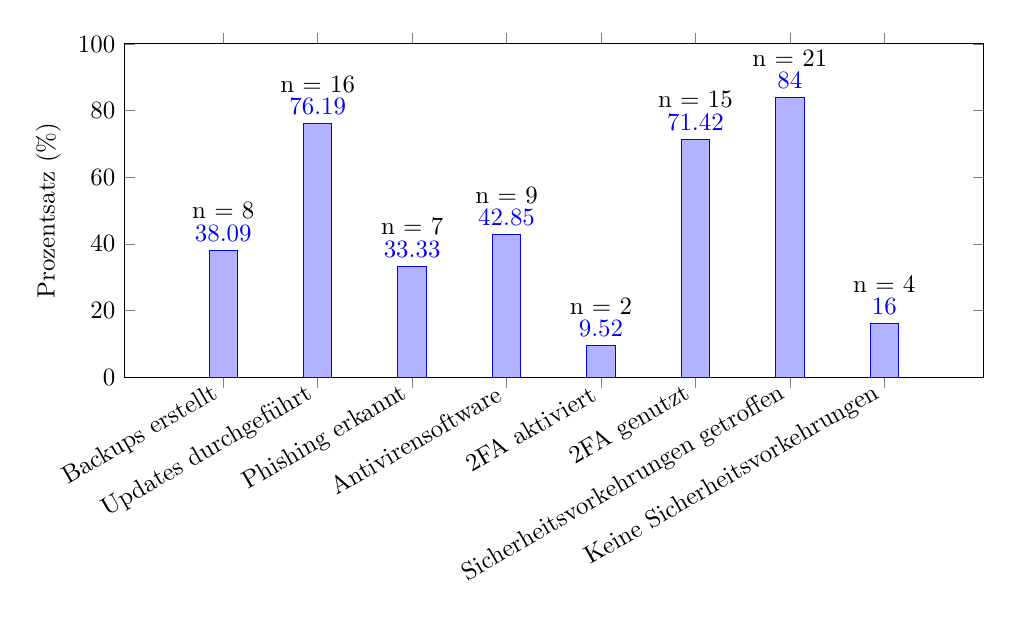
\begin{tikzpicture}[scale=0.9]
        \begin{axis}[
            ybar,
            symbolic x coords={Backups erstellt, Updates durchgeführt, Phishing erkannt, Antivirensoftware, 2FA aktiviert, 2FA genutzt, Sicherheitsvorkehrungen getroffen, Keine Sicherheitsvorkehrungen},
            xtick=data,
            nodes near coords,
            xlabel=,
            ylabel=Prozentsatz (\%),
            x tick label style={rotate=30, anchor=east},
            ymin=0, ymax=100, 
            enlarge x limits=0.15,
            width=\textwidth, 
            height=4.7cm, 
            scale only axis,
            bar width=0.4cm,
            every node near coord/.append style={anchor=south}, 
        ]
            \addplot coordinates {(Backups erstellt,38.09) (Updates durchgeführt,76.19) (Phishing erkannt,33.33) (Antivirensoftware,42.85) (2FA aktiviert,9.52) (2FA genutzt,71.42)
            (Sicherheitsvorkehrungen getroffen,84.00) (Keine Sicherheitsvorkehrungen,16.00)};

            \node[above=9pt] at (axis cs:Backups erstellt,38.09) {n = 8};
            \node[above=9pt] at (axis cs:Updates durchgeführt,76.19) {n = 16};
            \node[above=9pt] at (axis cs:Phishing erkannt,33.33) {n = 7};
            \node[above=9pt] at (axis cs:Antivirensoftware,42.85) {n = 9};
            \node[above=9pt] at (axis cs:2FA aktiviert,9.52) {n = 2};
            \node[above=9pt] at (axis cs:2FA genutzt,71.42) {n = 15};
            \node[above=9pt] at (axis cs:Sicherheitsvorkehrungen getroffen,84.00) {n = 21};
            \node[above=9pt] at (axis cs:Keine Sicherheitsvorkehrungen,16.00) {n = 4};
        \end{axis}
    \end{tikzpicture}
    \caption{Sicherheitsvorkehrungen der Studierenden in den letzten vier Wochen vor Umfragebeginn, einschließlich derjenigen, die keine Vorkehrungen getroffen haben (n = 25)}
\end{figure}

Von den Befragten haben 48\% Interesse an Schulungen gezeigt \((n=12)\), während 80\% die Wichtigkeit von IT-Sicherheit betonen \((n=20)\). Um Hilfe bei Problemen mit dem Computer, Laptop oder Smartphone zu bekommen verwendeten gaben 96\% der Befragten (\(n = 24\)) an, dass sie bei technischen Problemen Suchmaschinen verwenden. Von den Studierenden suchten 60\% \((n = 15)\) Rat bei Freunden, während 48\% \((n = 12)\) angaben, Hilfe von der Familie in Anspruch zu nehmen. Informationen auf FAU-Webseiten suchten 12\% \((n = 3)\), und IT-Techniker wurden von einer Person konsultiert. Print-Publikationen (z. B. Chip) wurden von 12\% \((n = 3)\) genutzt.\\
\\
72\% der Befragten haben Prokrastination (\(n = 18\)), 52\% Zeitmangel (\(n = 13\)) und 60\% Überforderung ihrer IT-Kenntnisse als Hindernisse genannt (\(n = 15\)). 12\% haben Angst oder Unsicherheit als Grund angegeben (\(n = 3\))
\\
Die folgende Grafik zeigt die prozentuale und absolute Verteilung der häufigsten Hindernisse für die Umsetzung von IT-Sicherheitsmaßnahmen:

\begin{figure}[H]
\centering
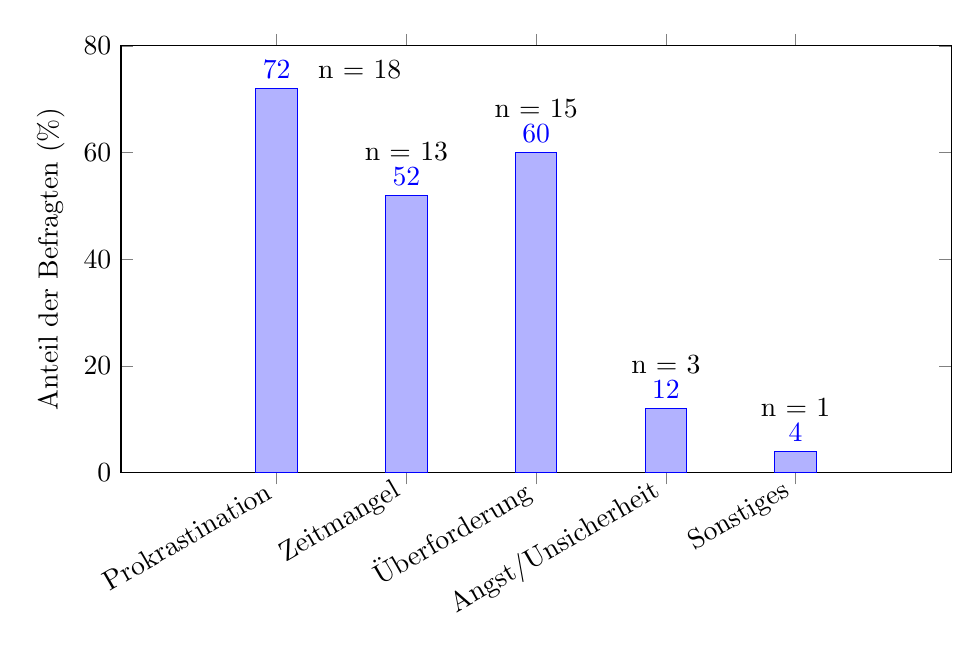
\begin{tikzpicture}
    \begin{axis}[
        ybar,
        symbolic x coords={Prokrastination, Zeitmangel, Überforderung, Angst/Unsicherheit, Sonstiges},
        xtick=data,
        ylabel={Anteil der Befragten (\%)},
        bar width=15pt,
        enlarge x limits=0.3,
        ymin=0,
        ymax=80,
        height=7cm,
        width=\textwidth,
        nodes near coords,
        nodes near coords align={vertical},
        x tick label style={rotate=30, anchor=east}
    ]
        \addplot coordinates {(Prokrastination,72) (Zeitmangel,52) (Überforderung,60) (Angst/Unsicherheit,12) (Sonstiges,4)};
        
        \node[above=0pt, xshift=30pt] at (axis cs:Prokrastination,72) {n = 18};
        \node[above=9pt] at (axis cs:Zeitmangel,52) {n = 13};
        \node[above=9pt] at (axis cs:Überforderung,60) {n = 15};
        \node[above=9pt] at (axis cs:Angst/Unsicherheit,12) {n = 3};
        \node[above=9pt] at (axis cs:Sonstiges,4) {n = 1};
    \end{axis}
\end{tikzpicture}
\caption{Hindernisse für die Umsetzung von IT-Sicherheitsmaßnahmen unter den Befragten (n = 25)}
\label{fig:hindernisse_it_sicherheit_balken}
\end{figure}

In der Kategorie „Sonstiges“ wurde von einer Person die ungünstige Planung von Updates als Hindernis angeführt.\\
\\
Zudem gaben 20\% der Befragten \((n=5)\) an, Opfer eines Cyberangriffs geworden zu sein.
\\
Von den Studierenden der Medizinischen Fakultät sehen 76\% einen Mehrwert in den Fachschaften \((n=19)\), während 24\% diesen nicht erkennen \((n=6)\).\\
\\
Einen Mehrwert darin, dass Fachschaften bei IT-Problemen unterstützen, sehen 84\% der Studierenden der Medizinischen Fakultät \((n=21)\).\\
\\
Die Webseite fau.info/infosec kannten 96\% der Befragten nicht \((n=24)\), während nur eine Person sie kannte.

\textit{Hinweis: Die Angaben beziehen sich auf die Antworten im folgendem Abschnitt. Es handelt sich hierbei um ein Ranking, bei dem die Teilnehmer die Möglichkeit hatten, zwischen 2 und 7 Antworten auszuwählen. Daher kann es vorkommen, dass nicht alle Teilnehmer alle Fragen beantwortet haben und die Summe der Prozentsätze und der absoluten Anzahl möglicherweise nicht genau 100\% bzw. die Gesamtzahl der Teilnehmer ergibt.}

Von den Medizinstudenten ordnen sich 28\% \((n=7)\) der Aussage „Ich mag es, wenn alles geordnet und nach Plan läuft“ zu, und ebenfalls 28\% \((n=7)\) ordnen sich der Aussage „Ich möchte, dass sich alle gut verstehen und mag keine Streits“ zu. Zudem geben 20\% \((n=5)\) der Studierenden an, dass „Ich liebe es, neue Dinge zu erleben und suche gerne Abenteuer“ auf sie zutrifft. Sicherheit und ein ruhiges Leben suchen 12\% \((n=3)\) der Studierenden und meiden Risiken. Von eine Person sagte jeweils, „Ich bin offen für neue Ideen und verschiedene Kulturen und mag Veränderungen“ auf sie zutrifft. Ebenfalls möcht ein Studierender „gerne führen und entscheiden und stehen gerne im Mittelpunkt“, und ein Weiterer „suchte nach Spaß und Spannung und probiere gerne Neues aus“.

\begin{figure}[H]
\centering
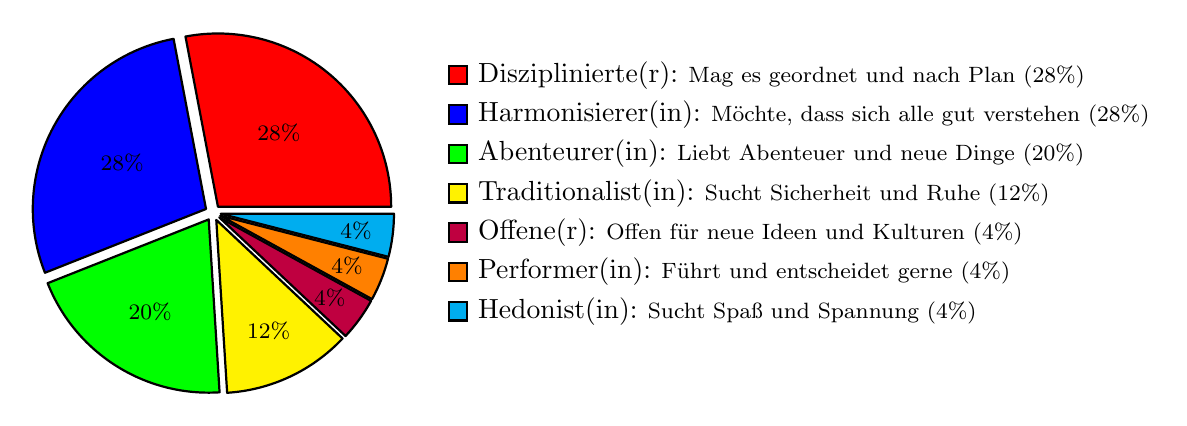
\begin{tikzpicture}
\pie[
    text=legend,
    radius=2.2,
    color={red, blue, green, yellow, purple, orange, cyan},
    explode=0.1,
    before number=\footnotesize,
    after number=\%,
    text=legend
]{
    28/Disziplinierte(r): \newline \footnotesize{ Mag es geordnet und nach Plan (28\%)},
    28/Harmonisierer(in): \newline \footnotesize{ Möchte, dass sich alle gut verstehen (28\%)},
    20/Abenteurer(in): \newline \footnotesize{ Liebt Abenteuer und neue Dinge (20\%)},
    12/Traditionalist(in): \newline \footnotesize{ Sucht Sicherheit und Ruhe (12\%)},
     4/Offene(r): \newline \footnotesize{ Offen für neue Ideen und Kulturen (4\%)},
     4/Performer(in): \newline \footnotesize{ Führt und entscheidet gerne (4\%)},
     4/Hedonist(in): \newline \footnotesize{ Sucht Spaß und Spannung (4\%)}
}
\end{tikzpicture}
\caption{Verteilung der Limbic Types \cite{hausel2011wissenschaftliche} unter Studierenden der Medizinischen Fakultät basierend auf ihren Aussagen (n = 25)}
\label{fig:limbic_types}
\end{figure}

\subsubsection{Offene Fragen - Medizinische Fakultät}

\textbf{Q1: Welche Gedanken und Gefühle kommen dir in den Sinn, wenn du an IT-Sicherheit denkst?}

In Bezug auf IT-Sicherheit berichteten Studierende der Medizinischen Fakultät von Frustration und Überforderung (n = 3). So äußerte ein Studierender: „Frustration, da immer ein Abwägen von Security und Bequemlichkeit.“ Ein weiterer Studierender sagte: „Überforderung, mangelndes Interesse, lästige Pflicht.“

Auch die Wichtigkeit und Notwendigkeit von IT-Sicherheitsmaßnahmen wurden von den Studierenden mehrfach betont (n = 3). Ein Studierender schrieb: „Wichtig, aber auch nervig, weil zeitraubend.“ Ein anderer sagte: „Muss gemacht werden, aber lästig in der Umsetzung.“

Praktische Maßnahmen, die ein Studierender ergriffen hat, um Risiken zu minimieren, wurden ebenfalls erwähnt. So äußerte dieser: „Interessantes Thema. Ich bin teilweise etwas paranoid deswegen, anstatt auf Links zu klicken (auch wenn sie von vertrauenswürdigen Adressen kommen), gehe ich auf die Webseite und suche dort das Ziel des Links.“

\textbf{Q2: Aus welchen Gründen könntest du dich gegen die Anwendung bestimmter Sicherheitsmaßnahmen entscheiden und warum würdest du trotzdem auf IT-Sicherheit Wert legen?}

Bequemlichkeit und Usability wurden als Gründe für die Nichtanwendung bestimmter Sicherheitsmaßnahmen genannt (n = 3). Ein Beispiel lautet: „ios-updates: Speicher voll.“ Ein weiterer Studierender erklärte: „Faulheit diese einzurichten.“

Ein Studierender gab an, dass IT-Sicherheitsmaßnahmen wichtig sind: „Zeitmangel zur Einrichtung, fehlende Kenntnisse; IT-Sicherheit ist ein notwendiger Schritt für Privacy.“

\textbf{Q3: Kennst du deutsche Universitäten, Hochschulen oder öffentliche Einrichtungen, die aufgrund von Cyberangriffen temporär ihren Betrieb einstellen mussten? Bitte beschreibe deine Kenntnisse oder Erlebnisse in diesem Zusammenhang.}

Mehrere Studierende gaben an, von Vorfällen gehört zu haben, bei denen Dienste an Universitäten zeitweise nicht mehr verfügbar waren (n = 4). Ein Studierender schrieb: „TH Nürnberg, Dienste waren zeitweise nicht mehr erreichbar (Studienselbstverwaltung etc).“ Ein anderer Studierender berichtete: „An meiner alten Hochschule, der Technischen Hochschule Ulm, gab es einen Cyberangriff, der zwar erkannt wurde, aber danach gingen monatelang die Remote-Verbindungen nicht mehr.“

Ein Studierender erwähnte den Verlust von Daten im Zusammenhang mit Cyberangriffen. Der Studierende bemerkte: „Man hört hin und wieder von Vorfällen, in denen Universitäten Opfer von Cyberattacken wurden und sensible Daten gestohlen oder die Infrastruktur lahm gelegt worden ist.“

\textbf{Q4: Was waren die Folgen des Cyberangriffs? (Wenn die Frage bejaht wurde, dass in der Familie jemand Opfer eines Cyberangriffs wurde.)}

Ein Studierender berichtete von Maßnahmen, die er nach einem Angriff ergriffen hat. Der Studierende schrieb: „DDoS eines Webservers. Führte dazu, dass ich Cloudflare angefangen habe zu nutzen.“ Ein weiterer Studierender berichtete von der Notwendigkeit, Systeme wiederherzustellen. Ein Beispiel lautet: „Als ich noch ein Kind war, hatten wir mal einen Trojaner auf dem Familien-PC, der dann den PC unbenutzbar gemacht hat. Mein Vater hat damals alles neu aufgesetzt und dann ging es wieder.“

\textbf{Q5: Aus welchen Gründen sollte die FAU der IT-Sicherheit eine hohe Priorität einräumen?}

Einige Studierende gaben den Schutz sensibler Daten als Grund an, warum die FAU der IT-Sicherheit eine hohe Priorität einräumen sollte (n = 4). Ein Studierender schrieb: „Weil Sicherheit von Daten (wissenschaftliche Daten und persönliche Daten der Beschäftigten und Studierenden) für eine Uni zentral ist. Die Uni besitzt sehr viele sensible Daten und stellt daher auch eine recht große Zielscheibe für Angreifer dar.“ Ein anderer meinte: „Schutz von Daten (sowohl persönliche Daten als auch Forschungsergebnisse etc.), Bewahrung von Handlungsfähigkeit/Schutz vor Störungen.“

\textbf{Q6: Gibt es Lehrstühle in deinem Fachbereich, die sich intensiv mit IT-Sicherheit beschäftigen? Falls ja, welche sind das und welche Maßnahmen ergreifen sie in diesem Bereich?}

Ein Studierender nannte einen Lehrstuhl: „Informatik Lehrstuhl 1.“ Ein weiterer Studierender äußerte, dass er keine entsprechenden Lehrstühle kenne.

\textbf{Q7: An welchen Stellen auf den Webseiten der FAU suchst du typischerweise nach Informationen zur IT-Sicherheit?}

Die Studierenden der Medizinischen Fakultät suchen meist nicht nach IT-Sicherheitsinformationen auf den Webseiten der FAU (n = 6). Ein Studierender sagte: „Gar nicht.“ Ein anderer erwähnte: „Ich versuche mich durchzuklicken, finde die FAU Website aber leider generell unübersichtlich.“

Einige Studierende nutzen das Rechenzentrum (n = 3), z. B. „Manchmal nutze ich die RRZE-Webseite.“

\subsection{Naturwissenschaftliche Fakultät}

\subsubsection{Geschlossene Fragen - Naturwissenschaftliche Fakultät}

Im Durchschnitt besitzen die Studierenden der Naturwissenschaftlichen Fakultät 3 (3.33) Geräte pro Person. Windows als Betriebssystem wird von 75.55\% \((n = 34)\) der Studierenden genutzt, während 24.44\% \((n = 11)\) Linux verwenden. macOS kommt bei 13.33\% \((n = 6)\) der Befragten zum Einsatz. Bei den Smartphones nutzen 80\% \((n = 36)\) Android und 20\% \((n = 9)\) iOS.

Von den Studierenden verwenden 60\% \((n=24)\) FAU-eigene VPN-Dienste und 70\% \((n=28)\) nutzen private VPNs. Außerdem nutzen 24\% \((n=13)\) der Befragten VPNs für die Arbeit. Ein Studierender ist sich unsicher, ob er VPNs verwendet hat und \(9.09\% \,(n = 4)\), haben noch nie einen VPN-Dienst benutzt.

Von den Befragten gaben 48.88\% an, für alle Konten unterschiedliche Passwörter zu verwenden \((n=22)\), und 48.88\% nutzen für einige wichtige Konten (z. B. Online-Banking) unterschiedliche Passwörter \((n=22)\). Ein Befragter verwendet für alle Konten das selbe Passwort.

Von den Studierenden gaben 73.33\% \((n=33)\) an, dass sie ihre Passwörter auswendig kennen, während 33.33\% \((n=15)\) ihre Passwörter schriftlich festhalten. Ebenfalls verwenden 35.35\% \((n=16)\) der Befragten digitale Passwort-Manager zur Verwaltung ihrer Zugangsdaten. Insgesamt speichern 15.55\% der Studierenden der Naturwissenschaftlichen Fakultät ihre Passwörter digital, beispielsweise in Textdokumenten wie Microsoft Word \((n=7)\), während 84.44\% \((n=38)\) diese Option nicht nutzen. Zudem sichern 35.55\% \((n=16)\) ihre Passwörter im Browser, während 64.44\% \((n=29)\) auf diese Methode verzichten.\\
\\
Die folgenden Angaben beziehen sich auf die von den Studierenden in den letzten vier Wochen vor Umfragebeginn getroffenen Sicherheitsvorkehrungen: 52.38\% der Befragten, die Sicherheitsvorkehrungen getroffen haben (\(n = 22\)), an, regelmäßig Backups zu erstellen, und 78.57\% (\(n = 33\)) führen regelmäßig Updates durch. 7.61\% (\(n = 3\)) der Befragten haben in diesem Zeitraum ein E-Mail-Zertifikat erstellt, und 88.09\% (\(n = 37\)) haben ein solches Zertifikat nicht genutzt. 54.76\% (\(n = 23\)) der Befragten erkannten Phishing-Versuche, jedoch meldeten nur 19.04\% (\(n = 8\)) diese Vorfälle.\\
\\
69.05\% (\(n = 29\)) der Befragten in der naturwissenschaftlichen Fakultät gaben an, keine Antivirensoftware zu verwenden, während 30.95\% (\(n = 13\)) dies tun. 76.19\% (\(n = 32\)) haben 2FA (Zwei-Faktor-Authentifizierung) nicht aktiviert, und 23.80\% (\(n = 10\)) haben dies getan. 61.90\% (\(n = 26\)) der Befragten gaben an, 2FA zu nutzen, während 38.09\% (\(n = 16\)) diese Sicherheitsmaßnahme nicht nutzen.\\
\\
85.71\% der Befragten (\(n = 36\)) gaben an, ihr WLAN nicht gesichert zu haben, während 14.28\% (\(n = 6\)) ihr WLAN gesichert haben. Schließlich erklärten 93.33\% (\(n = 42\)), dass sie Sicherheitsvorkehrungen getroffen haben, während 6.67\% (\(n = 3\)) angaben, keine solchen Vorkehrungen getroffen zu haben.\\
\\
Die folgende Grafik zeigt die prozentuale und absolute Verteilung der von den Studierenden in den letzten vier Wochen vor Umfragebeginn getroffenen Sicherheitsvorkehrungen in der naturwissenschaftlichen Fakultät:

\begin{figure}[H]
    \centering
    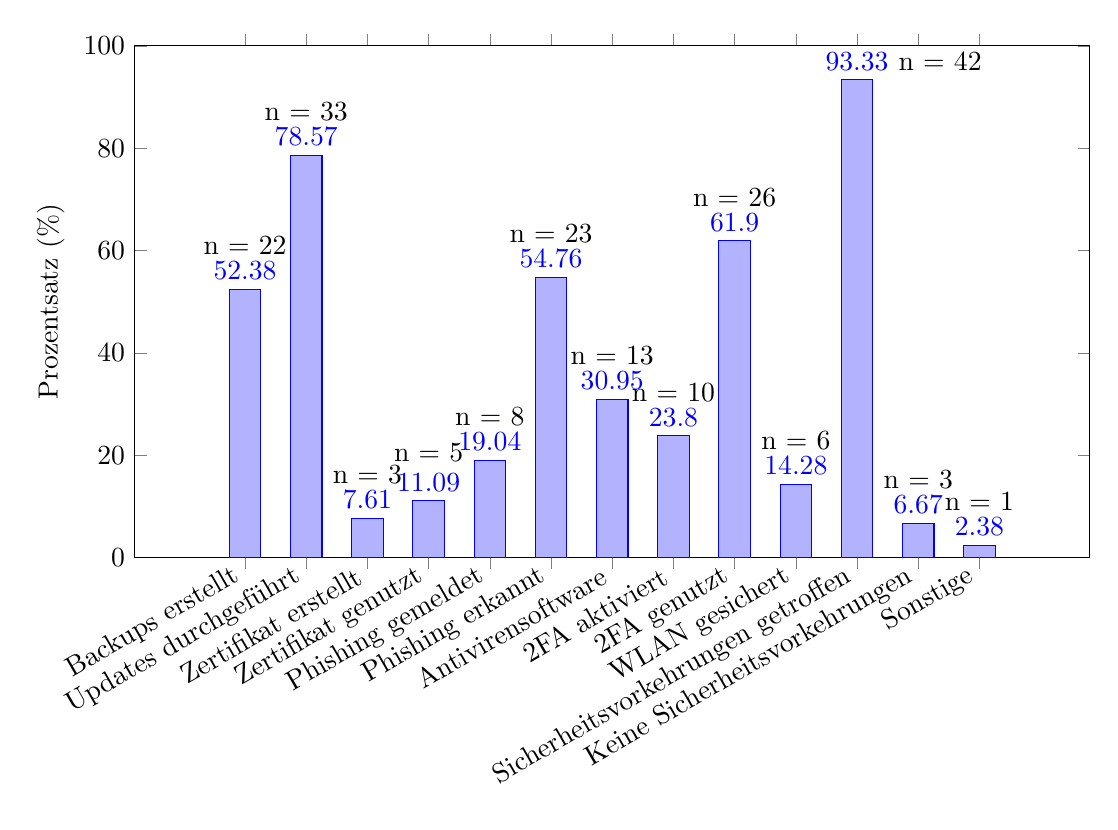
\begin{tikzpicture}
        \begin{axis}[
            ybar,
            symbolic x coords={Backups erstellt, Updates durchgeführt, Zertifikat erstellt, Zertifikat genutzt, Phishing gemeldet, Phishing erkannt, Antivirensoftware, 2FA aktiviert, 2FA genutzt, WLAN gesichert, Sicherheitsvorkehrungen getroffen, Keine Sicherheitsvorkehrungen, Sonstige},
            xtick=data,
            nodes near coords,
            xlabel=,
            ylabel=Prozentsatz (\%),
            x tick label style={rotate=30, anchor=east},
            ymin=0, ymax=100, 
            enlarge x limits=0.15,
            width=\textwidth,
            height=6.5cm, 
            scale only axis,
            bar width=0.4cm,
            every node near coord/.append style={anchor=south}, 
        ]
            \addplot coordinates {(Backups erstellt,52.38) (Updates durchgeführt,78.57) (Zertifikat erstellt,7.61) (Zertifikat genutzt,11.09) 
            (Phishing gemeldet,19.04) (Phishing erkannt,54.76) (Antivirensoftware,30.95) (2FA aktiviert,23.80) (2FA genutzt,61.90)
            (WLAN gesichert,14.28) (Sicherheitsvorkehrungen getroffen,93.33) (Keine Sicherheitsvorkehrungen,6.67) (Sonstige,2.38)};

            \node[above=9pt] at (axis cs:Backups erstellt,52.38) {n = 22};
            \node[above=9pt] at (axis cs:Updates durchgeführt,78.57) {n = 33};
            \node[above=9pt] at (axis cs:Zertifikat erstellt,7.61) {n = 3};
            \node[above=9pt] at (axis cs:Zertifikat genutzt,11.91) {n = 5};
            \node[above=9pt] at (axis cs:Phishing gemeldet,19.04) {n = 8};
            \node[above=9pt] at (axis cs:Phishing erkannt,54.76) {n = 23};
            \node[above=9pt] at (axis cs:Antivirensoftware,30.95) {n = 13};
            \node[above=9pt] at (axis cs:2FA aktiviert,23.80) {n = 10};
            \node[above=9pt] at (axis cs:2FA genutzt,61.90) {n = 26};
            \node[above=9pt] at (axis cs:WLAN gesichert,14.28) {n = 6};
            \node[above=0pt, xshift=30pt] at (axis cs:Sicherheitsvorkehrungen getroffen,93.33) {n = 42};
            \node[above=9pt] at (axis cs:Keine Sicherheitsvorkehrungen,6.67) {n = 3};
            \node[above=9pt] at (axis cs:Sonstige,2.38) {n = 1};
        \end{axis}
    \end{tikzpicture}
    \caption{Sicherheitsvorkehrungen der Studierenden in den letzten vier Wochen vor Umfragebeginn, einschließlich derjenigen, die keine Vorkehrungen getroffen haben (n = 45)}
\end{figure}

Unter „Sonstige“ gab jeweils ein Studierender folgende Antwort: „gmx (verschlüsselt)“, „automatische Windows-Updates“, und „ich würde das Standard-Passwort ändern“.\\
\\
Von den Befragten zeigen 64.44\% \((n = 29)\) Interesse an Schulungen, und 80\% \((n = 37)\) betonen die Wichtigkeit von IT-Sicherheit. Um Hilfe bei Problemen mit dem Computer, Laptop oder Smartphone zu bekommen verwendeten 91.11\% (\(n = 41\)) der Befragten, Suchmaschinen, während 44.44\% (\(n = 20\)) Rat bei Freunden suchten und 20.00\% (\(n = 9\)) Hilfe von der Familie in Anspruch nahmen. FAU-Seiten wurden von 15.55\% (\(n = 7\)) der Studierenden genutzt, und 17.77\% (\(n = 8\)) konsultierten IT-Techniker. Print-Publikationen wurden von 6.66\% \((n = 3)\) der Befragten verwendet. Zusätzlich wurden „Sonstige“-Antworten von 11.11\% \((n = 5)\) angegeben, darunter Beispiele wie „YouTube“ und „Stack Overflow“.\\
\\
73.68\% (\(n = 28\)) der Befragten nennen Prokrastination, 50\% (\(n = 19\)) Zeitmangel und 47.36\% (\(n = 18\)) Überforderung ihrer IT-Kenntnisse als Hindernisse. 10.52\% (\(n = 4\)) der Befragten geben Angst oder Unsicherheit als Grund an.\\
In der Kategorie „Sonstiges“ wurden Gründe wie Kosten, Unwissenheit über sinnvolle Maßnahmen und unpraktische Sicherheitslösungen \(11.11\% \,(n = 5)\) genannt.\\
\\
Die folgende Grafik zeigt die prozentuale und absolute Verteilung der häufigsten Hindernisse für die Umsetzung von IT-Sicherheitsmaßnahmen:

\begin{figure}[H]
\centering
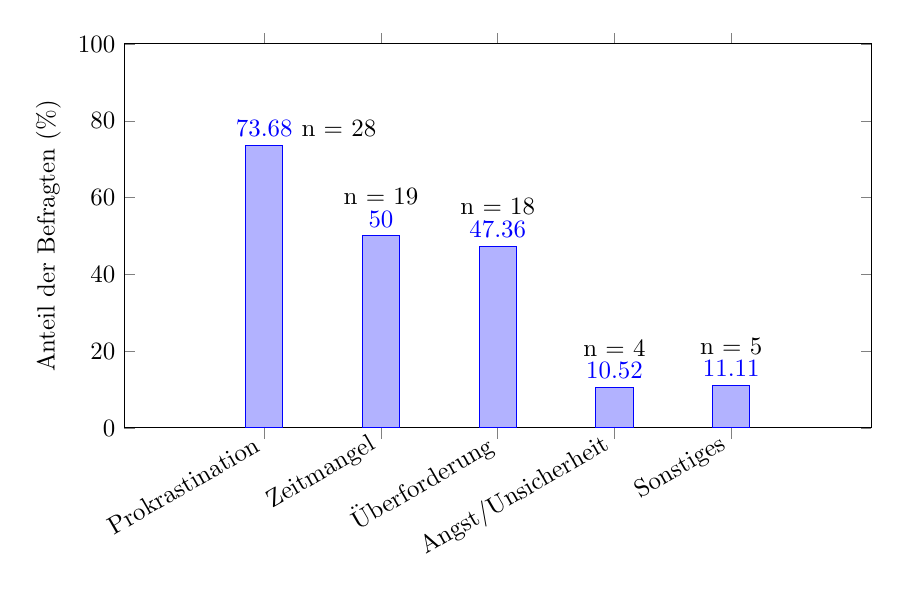
\begin{tikzpicture}[scale=0.9]
    \begin{axis}[
        ybar,
        symbolic x coords={Prokrastination, Zeitmangel, Überforderung, Angst/Unsicherheit, Sonstiges},
        xtick=data,
        ylabel={Anteil der Befragten (\%)},
        bar width=15pt,
        enlarge x limits=0.3,
        ymin=0,
        ymax=100,
        height=7cm,
        width=\textwidth,
        nodes near coords,
        nodes near coords align={vertical},
        x tick label style={rotate=30, anchor=east}
    ]
        \addplot coordinates {(Prokrastination,73.68) (Zeitmangel,50) (Überforderung,47.36) (Angst/Unsicherheit,10.52) (Sonstiges,11.11)};
        
        % Anzahl der Teilnehmer (n=) direkt über den Balken anzeigen
        \node[above=0pt, xshift=30pt] at (axis cs:Prokrastination,73.68) {n = 28};
        \node[above=9pt] at (axis cs:Zeitmangel,50) {n = 19};
        \node[above=9pt] at (axis cs:Überforderung,47.36) {n = 18};
        \node[above=9pt] at (axis cs:Angst/Unsicherheit,10.52) {n = 4};
        \node[above=9pt] at (axis cs:Sonstiges,11.11) {n = 5};
    \end{axis}
\end{tikzpicture}
\caption{Hindernisse für die Umsetzung von IT-Sicherheitsmaßnahmen unter den Befragten (n = 45)}
\label{fig:hindernisse_it_sicherheit_balken}
\end{figure}
\\
Zehn (22.22\%) der Befragten gaben an, Opfer eines Cyberangriffs geworden zu sein.
\\
Einen Mehrwert in den Fachschaften sehen 82.22\% \((n = 37)\) der Studierenden der Naturwissenschaftlichen Fakultät, während 17.78\% \((n = 8)\) diesen nicht erkennen. Unterstützung von Fachschaften bei IT-Problemen wünschen sich 62.22\% \((n = 28)\) der Befragten.\\
\\
Die Unterstützung von Fachschaften bei IT-Problemen befürworten 62.22\% \((n = 28)\) der Studierenden der Naturwissenschaftlichen Fakultät.\\
\\
Die Webseite fau.info/infosec kannten 86.66\% \((n = 39)\) der Befragten nicht, während 13.33\% \((n = 6)\) sie kannten.

\textit{Hinweis: Die Angaben beziehen sich auf die Antworten im folgendem Abschnitt. Es handelt sich hierbei um ein Ranking, bei dem die Teilnehmer die Möglichkeit hatten, zwischen 2 und 7 Antworten auszuwählen. Daher kann es vorkommen, dass nicht alle Teilnehmer alle Fragen beantwortet haben und die Summe der Prozentsätze und der absoluten Anzahl möglicherweise nicht genau 100\% bzw. die Gesamtzahl der Teilnehmer ergibt.}

Von den Studierenden ordnen sich 35.55\% \((n = 16)\) Aussagen wie „Ich mag es, wenn alles geordnet und nach Plan läuft und mag keine Überraschungen“ zu. Zudem geben 20.00\% \((n = 9)\) an, „Ich liebe es, neue Dinge zu erleben und suche gerne Abenteuer“. Weiterhin betonen 17.77\% \((n = 8)\), „Ich bin offen für neue Ideen und verschiedene Kulturen und mag Veränderungen“. Der Aussage „Ich möchte, dass sich alle gut verstehen und mag keine Streits“ ordnen sich 15.55\% \((n = 7)\) der Studierenden zu. Zudem suchen 6.66\% \((n = 3)\) „nach Spaß und Spannung und probiere gerne Neues aus“. Schließlich möchte ein Studierender „gerne führen und entscheiden und steht gerne im Mittelpunkt“, und ein weiterer sucht „Sicherheit, ein ruhiges Leben und meidet Risiken“.

\begin{figure}[H]
\centering
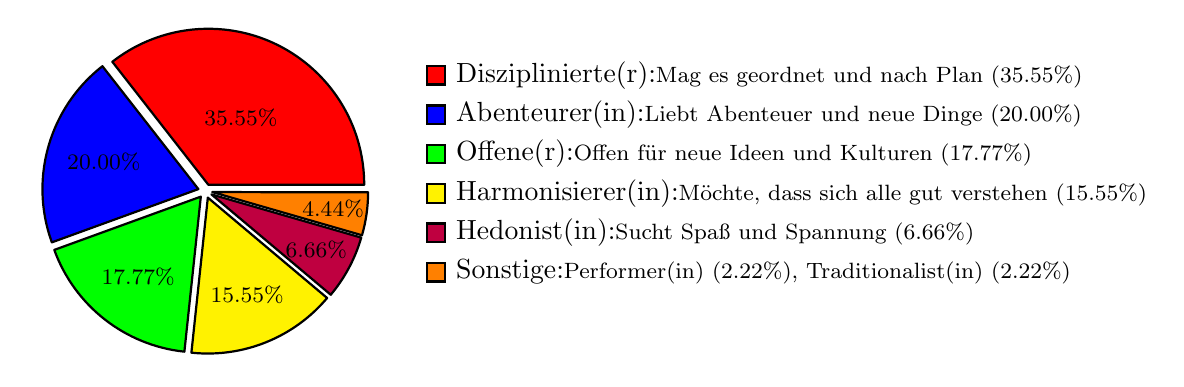
\begin{tikzpicture}[scale=0.9]
\pie[
    text=legend,
    radius=2.2,
    color={red, blue, green, yellow, purple, orange, cyan},
    explode=0.1,
    before number=\footnotesize,
    after number=\%,
    every slice/.style={font=\footnotesize},
    sum=100
]{
    35.55/Disziplinierte(r): \\ \footnotesize{Mag es geordnet und nach Plan (35.55\%)},
    20.00/Abenteurer(in): \\ \footnotesize{Liebt Abenteuer und neue Dinge (20.00\%)},
    17.77/Offene(r): \\ \footnotesize{Offen für neue Ideen und Kulturen (17.77\%)},
    15.55/Harmonisierer(in): \\ \footnotesize{Möchte, dass sich alle gut verstehen (15.55\%)},
    6.66/Hedonist(in): \\ \footnotesize{Sucht Spaß und Spannung (6.66\%)},
    4.44/Sonstige: \\ \footnotesize{Performer(in) (2.22\%), Traditionalist(in) (2.22\%)}
}
\end{tikzpicture}
\caption{Verteilung der Limbic Types \cite{hausel2011wissenschaftliche} unter Studierenden der Naturwissenschaftlichen Fakultät basierend auf ihren Aussagen (n = 45)}
\label{fig:limbic_types}
\end{figure}

\subsubsection{Offene Fragen - Naturwissenschaftliche Fakultät}

\textbf{Q1: Welche Gedanken und Gefühle kommen dir in den Sinn, wenn du an IT-Sicherheit denkst?}

In Bezug auf IT-Sicherheit berichteten zwei Studierende der Naturwissenschaftlichen Fakultät von Bedrohungen und Angst. Ein Studierender sagte: „Sicherheit von sensiblen Daten und Angst vor Hackangriffen.“ Ein weiterer Studierender meinte: „Man ist nie 100\% sicher.“

Misstrauen war ebenfalls ein genanntes Thema von zwei Studierenden. Ein Beispiel: „Abneigung gegenüber inkompetentem, paranoidem und überheblichem CISO.“ Ein anderer Studierender äußerte: „Ich bin mir bewusst darüber, dass meine Daten im Internet nicht gesichert sind und ich teilweise damit unsensibel umgehe.“

IT-Sicherheitsmaßnahmen wurden zwei Studierenden als relevant wahrgenommen. So bemerkte ein Studierender: „Ich sollte mehr machen.“

Bequemlichkeit und Komplexität wurden ebenfalls als Herausforderungen genannt. Ein Studierender äußerte sich wie folgt: „Zu komplex, um selber alles zu verstehen.“

\textbf{Q2: Aus welchen Gründen könntest du dich gegen die Anwendung bestimmter Sicherheitsmaßnahmen entscheiden und warum würdest du trotzdem auf IT-Sicherheit Wert legen?}

Bequemlichkeit und Usability wurden von zwei Studierenden als Gründe für die Ablehnung von Sicherheitsmaßnahmen genannt. Ein Studierender erklärte: „good enough... wenn mir der Aufwand zu groß wird, mach ich's nicht mehr. Ich werde sicher nicht mich jedes Mal neu anmelden bei einer Anwendung, die ich jede Stunde brauche.“

Weitere genannte Gründe waren jeweils mangelndes Wissen und Zeitmangel sowie der Aufwand, der mit der Implementierung von Sicherheitsmaßnahmen verbunden ist. Ein Beispiel lautet: „Wenn sie umständlich ist, z.B. 2FA-Code vom Handy eingeben oder KeePass öffnen muss.“

Andere Studierende nannten jeweils die Kosten oder das Misstrauen gegenüber digitalen Passwort-Managern als Gründe für die Ablehnung bestimmter Sicherheitsmaßnahmen.

\textbf{Q3: Kennst du deutsche Universitäten, Hochschulen oder öffentliche Einrichtungen, die aufgrund von Cyberangriffen temporär ihren Betrieb einstellen mussten?}

Studierende der Naturwissenschaftlichen Fakultät berichteten gleichermaßen von Kenntnissen über solche Vorfälle (n = 4) und von fehlenden Kenntnissen (n = 4). Beispiele für positive Antworten waren: „Ja ab und zu lese ich davon, und ich bin mir des Risikos bewusst.“ Ein anderer Studierender erwähnte die „Frankfurter University of Applied Science: Erkenntnis aus Zeitung.“

\textbf{Q4: Was waren die Folgen des Cyberangriffs? (Wenn die Frage bejaht wurde, dass in der Familie jemand Opfer eines Cyberangriffs wurde.)}

Zwei Studierende berichteten von Verlusten des Kontos oder Zugangs. So schrieb ein Studierender: „Ich musste mir in einem Spiel einen neuen Account zulegen.“ Ein weiterer Studierender bemerkte: „Windows TeamViewer-Übernahme eines Kollegen. Löschung des kompromittierten Microsoft-Kontos.“

Weitere genannte Folgen waren jeweils ein Betriebsausfall oder Lahmlegung, Identitätsdiebstahl oder unautorisierte Nutzung sowie das Auftreten von mehr Spam. Ein Studierender berichtete zudem von der Notwendigkeit einer Systemwiederherstellung.

\textbf{Q5: Aus welchen Gründen sollte die FAU der IT-Sicherheit eine hohe Priorität einräumen?}

Der Schutz sensibler Daten wurde als wichtiger Grund genannt (n = 4). Ein Studierender schrieb: „Im Informationszeitalter ist nichts so wichtig wie Information.“ Ein anderer betonte: „Data of students.“

Weitere genannte Gründe waren die Verhinderung von Betriebsunterbrechungen und der Schutz vor finanziellen Schäden (jeweils von zwei Studierenden genannt). Ein Studierender bemerkte: „IT-Sicherheit lässt sich einplanen, Schäden durch erfolgreiche Angriffe nicht.“

\textbf{Q6: Gibt es Lehrstühle in deinem Fachbereich, die sich intensiv mit IT-Sicherheit beschäftigen? Falls ja, welche sind das und welche Maßnahmen ergreifen sie in diesem Bereich?}

Studierende der Naturwissenschaftlichen Fakultät gaben an, keine Lehrstühle zu kennen, die sich intensiv mit IT-Sicherheit beschäftigen (n = 4). Ein Studierender schrieb: „Weiß ich nicht.“

Zwei Studierende nannten jedoch spezifische Lehrstühle oder Maßnahmen. Ein Beispiel lautet: „Kenne nur den Kryptographie-Lehrstuhl von Prof. Schröder.“ Ein weiterer Studierender erwähnte durchgeführte Maßnahmen: „I1 z.B. Poster aufhängen.“

\textbf{Q7: An welchen Stellen auf den Webseiten der FAU suchst du typischerweise nach Informationen zur IT-Sicherheit?}

Die Studierenden der Naturwissenschaftlichen Fakultät suchen hauptsächlich auf den Seiten des Rechenzentrums (RRZE) nach IT-Sicherheitsinformationen (n = 11). Ein Studierender erklärte: „Auf den Webseiten des RRZE.“ Ein anderer sagte: „Wenn überhaupt, dann auf den Seiten des RRZE wo auch Infos zu meinen Zugängen usw stehen.“

Einige Studierende gaben an, keine spezifischen Informationen zur IT-Sicherheit zu suchen (n = 3). Einer sagte: „Gar nicht.“ Ein Studierender erwähnte, dass er Informationen per E-Mail erhält.

\subsection{Philosophische Fakultät / Fachbereich Theologie}

\subsubsection{Geschlossene Fragen - Philosophische Fakultät / Fachbereich Theologie}

Die Studierenden der Philosophischen Fakultät / Fachbereich Theologie haben 3 (3.08) Geräte pro Person. Von den Studierenden nutzen 91.66\% \((n = 33)\) Windows als Betriebssystem, ein Studierender verwendet Linux und 16.66\% \((n = 6)\) macOS. Die Smartphones der Teilnehmer sind auf Android \((58.33\%, n = 21)\) und iOS \((38.88\%, n = 14)\) verteilt. Ein Teilnehmer gab an, Ubuntu Touch zu verwenden, ein Weiterer gab an, kein Smartphone zu besitzen.\\
\\
Von den Studierenden geben 34.37\% \((n = 11)\) an, private VPNs zu nutzen, und 21.87\% \((n = 7)\) verwenden VPNs für die Arbeit. FAU-eigene VPN-Dienste werden von 84.37\% \((n = 27)\) der Studierenden genutzt. Insgesamt 11.11\% \((n = 4)\) gaben an, keinen VPN-Dienst zu nutzen.\\
\\
Von den Befragten geben 58.33\% \((n=21)\) an, für all ihre Konten unterschiedliche Passwörter zu nutzen. Ebenso nutzen 36.11\% \((n=13)\) für einige besonders wichtige Konten, wie etwa für das Online-Banking, unterschiedliche Passwörter. Zwei Studierende verwenden dasselbe Passwort für alle Konten.\\
\\
Von den Studierenden gaben 63.88\% \((n=23)\) an, dass sie ihre Passwörter auswendig kennen, während 41.66\% \((n=15)\) ihre Passwörter schriftlich festhalten. Zudem verwenden 33.33\% \((n=15)\) der Befragten digitale Passwort-Manager zur Verwaltung ihrer Zugangsdaten. Drei der Studierenden 8.33\% \((n=3)\) der Philosophischen Fakultät speichern ihre Passwörter digital, beispielsweise in Textdokumenten wie Microsoft Word. Außerdem sichern 36.11\% \((n=13)\) ihre Passwörter im Browser.\\
Eine Person gab an: „Ich vergesse sie und setze sie jedes Mal zurück (kenne fast nur meine E-Mail-Adresse auswendig).“\\
\\
Die folgenden Angaben beziehen sich auf die von den Studierenden in den letzten vier Wochen vor Umfragebeginn getroffenen Sicherheitsvorkehrungen: 25.00\% der Befragten, die Sicherheitsvorkehrungen getroffen haben (\(n = 32\)), an, regelmäßig Backups zu erstellen, und 78.12\% (\(n = 25\)) führen regelmäßig Updates durch. \textbf{Keiner} der Befragten hat in diesem Zeitraum ein E-Mail-Zertifikat erstellt oder genutzt. 31.25\% (\(n = 10\)) der Befragten erkannten Phishing-Versuche, jedoch meldeten 90.62\% (\(n = 29\)) diese Vorfälle nicht.\\
\\
65.62\% (\(n = 21\)) der Befragten gaben an, keine Antivirensoftware zu verwenden, während 34.37\% (\(n = 11\)) dies tun. 78.12\% (\(n = 25\)) haben 2FA (Zwei-Faktor-Authentifizierung) nicht aktiviert, und 21.87\% (\(n = 7\)) haben dies getan. 59.37\% (\(n = 19\)) der Befragten gaben an, 2FA zu nutzen, während 40.62\% (\(n = 13\)) diese Sicherheitsmaßnahme nicht nutzen.\\
\\
93.75\% der Befragten (\(n = 30\)) gaben an, ihr WLAN nicht gesichert zu haben, während 6.25\% (\(n = 2\)) ihr WLAN gesichert haben. Schließlich erklärten 88.88\% (\(n = 32\)), dass sie Sicherheitsvorkehrungen getroffen haben, während 11.11\% (\(n = 4\)) angaben, keine solchen Vorkehrungen getroffen zu haben.\\
\\
Die folgende Grafik zeigt die prozentuale und absolute Verteilung der von den Studierenden in den letzten vier Wochen vor Umfragebeginn getroffenen Sicherheitsvorkehrungen:

\begin{figure}[H]
    \centering
    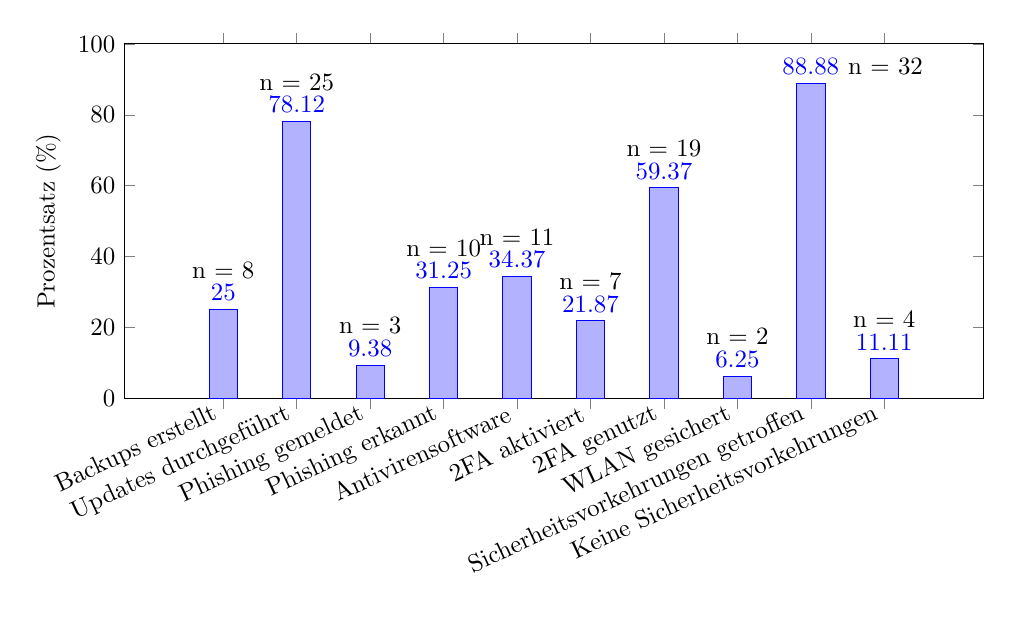
\begin{tikzpicture}[scale=0.9]
        \begin{axis}[
            ybar,
            symbolic x coords={Backups erstellt, Updates durchgeführt, Phishing gemeldet, Phishing erkannt, Antivirensoftware, 2FA aktiviert, 2FA genutzt, WLAN gesichert, Sicherheitsvorkehrungen getroffen, Keine Sicherheitsvorkehrungen},
            xtick=data,
            nodes near coords,
            xlabel=,
            ylabel=Prozentsatz (\%),
            x tick label style={rotate=25, anchor=east},
            ymin=0, ymax=100,
            enlarge x limits=0.15,
            width=\textwidth,
            height=5cm,
            scale only axis,
            bar width=0.4cm,
            every node near coord/.append style={anchor=south},
        ]
            \addplot coordinates {(Backups erstellt,25.00) (Updates durchgeführt,78.12)
            (Phishing gemeldet,9.38) (Phishing erkannt,31.25) (Antivirensoftware,34.37) (2FA aktiviert,21.87) (2FA genutzt,59.37)
            (WLAN gesichert,6.25) (Sicherheitsvorkehrungen getroffen,88.88) (Keine Sicherheitsvorkehrungen,11.11)};

            \node[above=9pt] at (axis cs:Backups erstellt,25.00) {n = 8};
            \node[above=9pt] at (axis cs:Updates durchgeführt,78.12) {n = 25};
            \node[above=9pt] at (axis cs:Phishing gemeldet,9.37) {n = 3};
            \node[above=9pt] at (axis cs:Phishing erkannt,31.25) {n = 10};
            \node[above=9pt] at (axis cs:Antivirensoftware,34.37) {n = 11};
            \node[above=9pt] at (axis cs:2FA aktiviert,21.87) {n = 7};
            \node[above=9pt] at (axis cs:2FA genutzt,59.37) {n = 19};
            \node[above=9pt] at (axis cs:WLAN gesichert,6.25) {n = 2};
            \node[above=0pt, xshift=30pt] at (axis cs:Sicherheitsvorkehrungen getroffen,88.88) {n = 32};
            \node[above=9pt] at (axis cs:Keine Sicherheitsvorkehrungen,11.11) {n = 4};
        \end{axis}
    \end{tikzpicture}
    \caption{Sicherheitsvorkehrungen der Studierenden in den letzten vier Wochen vor Umfragebeginn, einschließlich derjenigen, die keine Vorkehrungen getroffen haben (n = 36)}
\end{figure}

Von den Befragten zeigen 50\% \((n = 18)\) Interesse an Schulungen, und 88.87\% \((n = 32)\) stimmen der Wichtigkeit von IT-Sicherheit zu.\\
\\
Um Hilfe bei Problemen mit dem Computer, Laptop oder Smartphone zu bekommen verwendeten 91.66\% (\(n = 33\)) Suchmaschinen, während 58.33\% (\(n = 21\)) Rat bei Freunden suchten. Familienmitglieder wurden von 33.33\% (\(n = 12\)) konsultiert, und 16.66\% (\(n = 6\)) suchten auf FAU-Seiten nach Informationen. Insgesamt 8.33\% \((n = 3)\) der Befragten gaben an, IT-Techniker zu konsultieren, und zwei Studierende nutzten Print-Publikationen. Weitere 8.33\% \((n = 3)\) gaben „Sonstige“-Antworten an, wie z. B. „mein Freund ist Informatiker“ und „YouTube Erklärvideos“.\\
\\
75\% (\(n = 27\)) der Befragten nennen Prokrastination, 27.77\% (\(n = 10\)) Zeitmangel und 47.22\% (\(n = 17\)) Überforderung ihrer IT-Kenntnisse als Hindernisse. 19.44\% (\(n = 7\)) der Befragten geben Angst oder Unsicherheit als Grund an.
\\
Die folgende Grafik zeigt die prozentuale und absolute Verteilung der häufigsten Hindernisse für die Umsetzung von IT-Sicherheitsmaßnahmen:

\begin{figure}[H]
\centering
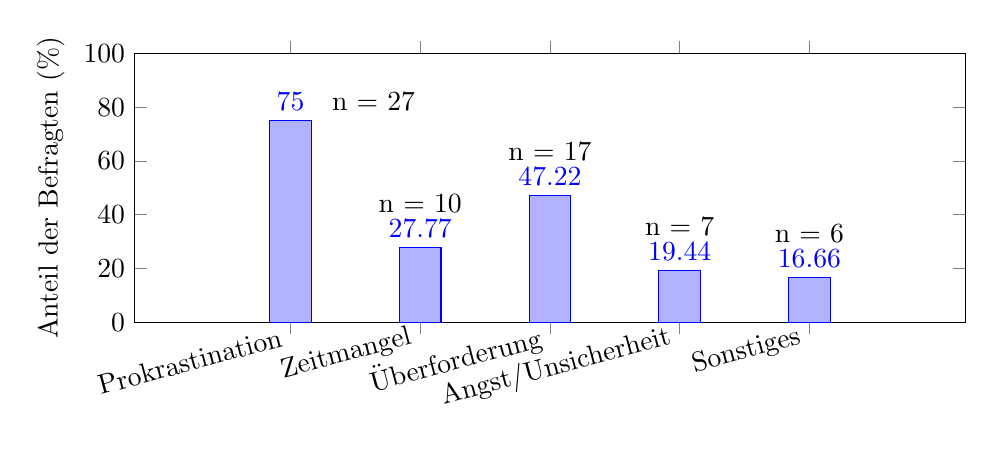
\begin{tikzpicture}
    \begin{axis}[
        ybar,
        symbolic x coords={Prokrastination, Zeitmangel, Überforderung, Angst/Unsicherheit, Sonstiges},
        xtick=data,
        ylabel={Anteil der Befragten (\%)},
        bar width=15pt,
        enlarge x limits=0.3,
        ymin=0,
        ymax=100,
        height=5cm,
        width=\textwidth,
        nodes near coords,
        nodes near coords align={vertical},
        x tick label style={rotate=15, anchor=east}
    ]
        \addplot coordinates {(Prokrastination,75) (Zeitmangel,27.77) (Überforderung,47.22) (Angst/Unsicherheit,19.44) (Sonstiges,16.66)};
        
        % Anzahl der Teilnehmer (n=) direkt über den Balken anzeigen
        \node[above=0pt, xshift=30pt] at (axis cs:Prokrastination,75) {n = 27};
        \node[above=9pt] at (axis cs:Zeitmangel,27.77) {n = 10};
        \node[above=9pt] at (axis cs:Überforderung,47.22) {n = 17};
        \node[above=9pt] at (axis cs:Angst/Unsicherheit,19.44) {n = 7};
        \node[above=9pt] at (axis cs:Sonstiges,16.66) {n = 6};
    \end{axis}
\end{tikzpicture}
\caption{Hindernisse für die Umsetzung von IT-Sicherheitsmaßnahmen unter den Befragten (n = 36)}
\label{fig:hindernisse_it_sicherheit_balken}
\end{figure}

In der Kategorie „Sonstiges“ \(16.66\% \,(n = 6)\) wurden Gründe wie fehlende verlässliche Quellen, Faulheit oder die hohen Kosten von Sicherheitssoftware genannt.\\
\\
Es gaben 19.44\% \((n = 7)\) der Befragten an, Opfer eines Cyberangriffs geworden zu sein.
\\
Einen Mehrwert in den Fachschaften sehen 69.44\% \((n = 25)\) der Studierenden der Philosophischen Fakultät, während 30.56\% \((n = 11)\) diesen nicht erkennen.\\
\\
Die Unterstützung von Fachschaften bei IT-Problemen befürworten 63.88\% \((n = 23)\) der Studierenden der Philosophischen Fakultät.\\
\\
Die Webseite fau.info/infosec kannten 94.44\% \((n = 34)\) der Befragten nicht, während zwei der Studierenden sie kannten.\\
\\
\textit{Hinweis: Die Angaben beziehen sich auf die Antworten im folgendem Abschnitt. Es handelt sich hierbei um ein Ranking, bei dem die Teilnehmer die Möglichkeit hatten, zwischen 2 und 7 Antworten auszuwählen. Daher kann es vorkommen, dass nicht alle Teilnehmer alle Fragen beantwortet haben und die Summe der Prozentsätze und der absoluten Anzahl möglicherweise nicht genau 100\% bzw. die Gesamtzahl der Teilnehmer ergibt.}\\
\\
Von den Studierenden ordnen sich 30.55\% \((n = 11)\) der Aussage „Ich bin offen für neue Ideen und verschiedene Kulturen und mag Veränderungen“ zu. Zudem geben 19.44\% \((n = 7)\) an, „Ich mag es, wenn alles geordnet und nach Plan läuft und mag keine Überraschungen“. Weitere 19.44\% \((n = 7)\) der Studierenden ordnen sich der Aussage „Ich suche Sicherheit und ein ruhiges Leben und meide Risiken“ zu. Der Aussage „Ich möchte, dass sich alle gut verstehen und mag keine Streits“ ordnen sich 16.66\% \((n = 6)\) der Studierenden zu. Zudem geben 8.33\% \((n = 3)\) an, „Ich liebe es, neue Dinge zu erleben und suche gerne Abenteuer“. Schließlich ordnen sich zwei Studierende der Aussage „Ich suche nach Spaß und Spannung und probiere gerne Neues aus“ zu.

\begin{figure}[H]
\centering
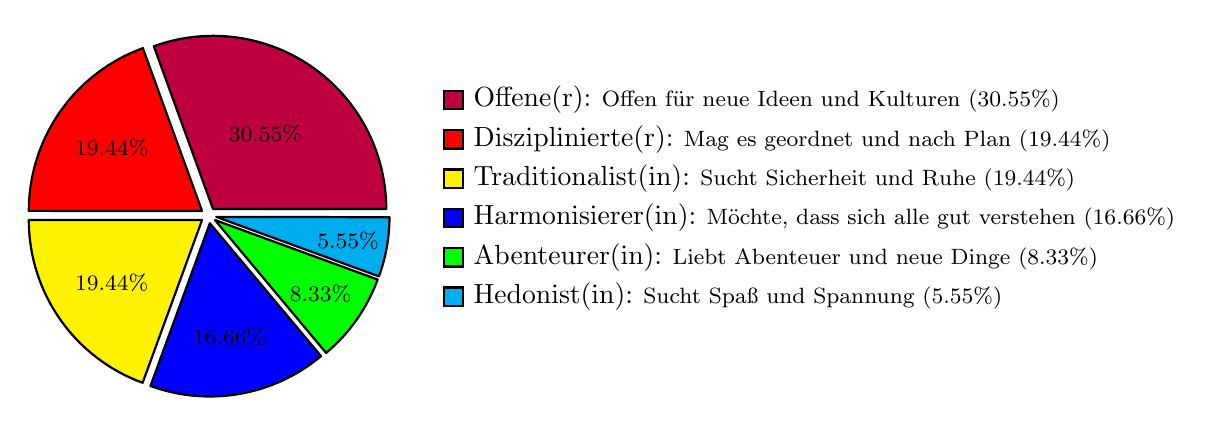
\begin{tikzpicture}
\pie[
    text=legend,
    radius=2.2,
    color={purple, red, yellow, blue, green, cyan},
    explode=0.1,
    before number=\footnotesize,
    after number=\%,
    text=legend
]{
    30.55/Offene(r): \newline \footnotesize{ Offen für neue Ideen und Kulturen (30.55\%)},
    19.44/Disziplinierte(r): \newline \footnotesize{ Mag es geordnet und nach Plan (19.44\%)},
    19.44/Traditionalist(in): \newline \footnotesize{ Sucht Sicherheit und Ruhe (19.44\%)},
    16.66/Harmonisierer(in): \newline \footnotesize{ Möchte, dass sich alle gut verstehen (16.66\%)},
     8.33/Abenteurer(in): \newline \footnotesize{ Liebt Abenteuer und neue Dinge (8.33\%)},
     5.55/Hedonist(in): \newline \footnotesize{ Sucht Spaß und Spannung (5.55\%)}
}
\end{tikzpicture}
\caption{Verteilung der Limbic Types \cite{hausel2011wissenschaftliche} unter Studierenden der Philosophischen Fakultät / Fachbereich Theologie basierend auf ihren Aussagen (n = 36)}
\label{fig:limbic_types}
\end{figure}

\subsubsection{Offene Fragen - Philosophische Fakultät / Fachbereich Theologie}

\textbf{Q1: Welche Gedanken und Gefühle kommen dir in den Sinn, wenn du an IT-Sicherheit denkst?}

Studierende der Philosophischen Fakultät/Fachbereich Theologie berichteten von Frustration und Überforderung (n = 3). Ein Studierender sagte: „Es ist überwältigend und unübersichtlich. Ich erkenne nicht, ob etwas sicher ist oder nicht.“ Ein anderer meinte: „Überforderung, scheint wie so ein riesiges undurchsichtiges Feld. Außerdem denke ich, dass ein sicherer Umgang viel Geld kostet.“

Bedrohungen und Angst wurde ebenfalls einmalig genannt. So wurde geäußert: „Ich hoffe, ich habe keine Viren auf meinem Computer durch das Ausführen von heruntergeladenen Spielen.“

Ein weiterer Studierender sprach von Bedrohungen und hob die Komplexität des Themas hervor: „Russland, Bürokratie- und Papier-Monster Deutschland, Faxgeräte, soll eigentlich für alle Grundwissen sein, KI ist gefährlich (Stimm- und Datenmanipulationen).“

\textbf{Q2: Aus welchen Gründen könntest du dich gegen die Anwendung bestimmter Sicherheitsmaßnahmen entscheiden und warum würdest du trotzdem auf IT-Sicherheit Wert legen?}

Sicherheitsbewusstsein sowie Bequemlichkeit und Usability wurden von zwei Studierenden als Gründe für die Entscheidung gegen bestimmte Sicherheitsmaßnahmen genannt. Ein Studierender erklärte: „Zeitersparnis, insbesondere da die meisten kostenlosen Passwortmanager nicht auf Android, Mac und Windows funktionieren.“ Ein weiterer Studierender meinte: „Aufgrund von Zeitmangel und oft auch Prokrastination: zu selten Backups machen.“

Ein Studierender erwähnte die Bedeutung der IT-Sicherheit, gab aber den Aufwand als Hindernis an: „Zeitmangel, Nutzen nicht klar ersichtlich; ich möchte natürlich trotzdem, dass mein Rechner reibungslos funktioniert und meine Daten nicht verloren gehen.“

\textbf{Q3: Kennst du deutsche Universitäten, Hochschulen oder öffentliche Einrichtungen, die aufgrund von Cyberangriffen temporär ihren Betrieb einstellen mussten?}

Vier Studierende berichteten, von solchen Vorfällen gehört zu haben (n = 4). Ein Studierender erwähnte: „Ja, öffentliche Einrichtung in der Stadt Nürnberg. Der Angriff erfolgte über einen längeren Zeitraum von mehreren Wochen. Nach und nach wurde die E-Mail-Kommunikationsstruktur, Aufgaben, verwendete Schreibweisen und zuständige Personen kompromittiert.“ Ein weiterer Studierender sagte: „Ich habe auf jeden Fall schon häufiger drüber gelesen, auch wenn ich jetzt nicht mehr weiß, bei welchen Einrichtungen genau.“

\textbf{Q4: Was waren die Folgen des Cyberangriffs? (Wenn die Frage bejaht wurde, dass in der Familie jemand Opfer eines Cyberangriffs wurde.)}

Ein Studierender berichtete von einem finanziellen Schaden: „Meine Mutter hat auf einer fake eBay-Seite ‚bestellt‘ und 4000€ verloren (falsche Bestellung bei MediaMarkt), weil sie auch ihre Bankdaten angegeben hatte.“ Ein anderer Studierender sprach von einem Verlust des Kontos oder Zugangs: „Bekannte waren von Phishing betroffen und haben Zugriff auf ihr Bankkonto verloren.“

\textbf{Q5: Aus welchen Gründen sollte die FAU der IT-Sicherheit eine hohe Priorität einräumen?}

Der Schutz sensibler Daten wurde von zwei Studierenden als Grund angegeben. Ein Studierender schrieb: „Es geht nicht nur um die Institution, sondern auch um das Privatleben der einzelnen Studenten/Mitarbeiter sicher zu halten. Die durchschnittliche Attacke manipuliert das Opfer emotional.“

Ein Studierender hob die Bedeutung von Schulungen und Awareness hervor: „Awareness kann leicht geschult werden, was es einfacher macht, Präventionsmaßnahmen durchzuführen.“

Die Verhinderung von Betriebsunterbrechungen wurde ebenfalls einmalig genannt: „Schlechte IT-Sicherheit an der FAU würde ein hohes Risiko für alle Beteiligten darstellen. Man hört in den Medien von anderen Universitäten, welche gravierenden Auswirkungen teils durch mangelnde IT-Sicherheit hervorgehen (z.B. Datendiebstahl, keine Verfügbarkeit der Uni-Systeme).“

Reputation und Professionalität wurde von einem Studierenden als relevanter Faktor benannt: „Fände es unprofessionell, wenn sie es nicht täte.“

\textbf{Q6: Gibt es Lehrstühle in deinem Fachbereich, die sich intensiv mit IT-Sicherheit beschäftigen? Falls ja, welche sind das und welche Maßnahmen ergreifen sie in diesem Bereich?}

Drei Studierenden gaben an, keine Lehrstühle zu kennen, die sich intensiv mit IT-Sicherheit beschäftigen (n = 3). Ein Studierender sagte: „Ich studiere an der Philosophischen Fakultät und weiß nichts von Lehrstühlen, die sich intensiv mit dem Thema beschäftigen.“

\textbf{Q7: An welchen Stellen auf den Webseiten der FAU suchst du typischerweise nach Informationen zur IT-Sicherheit?}

Die Mehrheit der Studierenden der Philosophischen Fakultät / Fachbereich Theologie gab an, keine spezifischen Informationen zur IT-Sicherheit auf den Webseiten der FAU zu suchen (n = 13). Ein Studierender sagte: „Gar nicht.“ Ein anderer bemerkte: „Ich habe noch nie nach derartigen Informationen gesucht.“

Einige Studierende nutzen das Rechenzentrum (n = 5).

\subsection{Rechts- und Wirtschaftswissenschaftliche Fakultät}

\subsubsection{Geschlossene Fragen - Rechts- und Wirtschaftswissenschaftliche Fakultät}

Die Studierenden der Rechts- und Wirtschaftswissenschaftlichen Fakultät haben 3 (3.03) Geräte pro Person. Insgesamt verwenden 83.33\% \((n = 30)\) der Studierenden Windows als Betriebssystem, während Linux \((8.33\%, n = 3)\) und macOS \((30.55\%, n = 11)\) weniger verbreitet sind. Bei den Smartphones nutzen 61.11\% \((n = 22)\) Android und 38.88\% \((n = 14)\) iOS. Ein Studierender gab an, Lineage OS auf seinem Smartphone zu verwenden \((2.77\%, n = 1)\).\\
\\
Von den Studierenden nutzen 55.88\% \((n = 19)\) private VPNs, und 35.29\% \((n = 12)\) verwenden VPNs für die Arbeit. Zudem nutzen 73.52\% \((n = 25)\) der Studierenden FAU-eigene VPN-Dienste. Eine Person, gab an keinen VPN-Dienst zu nutzen, eine weitere ist sich unsicher, ob sie einen VPN verwendet hat \\
\\
Von den Befragten gaben 61.11\% \((n=22)\) an, für alle ihre Konten unterschiedliche Passwörter zu verwenden. Weitere 33.33\% \((n=12)\) nutzen für besonders wichtige Konten, wie beispielsweise für Online-Banking, separate Passwörter. Zwei der Befragten verwenden dasselbe Passwort für alle ihre Konten.\\
\\
Von den Befragten gaben 52.77\% \((n=19)\) an, ihre Passwörter auswendig zu kennen, während 25\% \((n=9)\) sie schriftlich festhalten. Darüber hinaus verwenden 47.22\% \((n=17)\) der Studierenden digitale Passwort-Manager, um ihre Zugangsdaten zu verwalten. Zudem speichern 8.33\% \((n=3)\) der Befragten ihre Passwörter digital, beispielsweise in Programmen wie Microsoft Word. Des Weiteren sichern 50.00\% \((n=18)\) der Befragten ihre Passwörter im Browser.
Ein Studierender gab an, „NitroKey“ zu nutzen.\\
\\
Die folgenden Angaben beziehen sich auf die von den Studierenden in den letzten vier Wochen vor Umfragebeginn getroffenen Sicherheitsvorkehrungen: 38.23\% der Befragten, die Sicherheitsvorkehrungen getroffen haben (\(n = 34\)), gaben an, regelmäßig Backups zu erstellen, und 79.41\% (\(n = 27\)) führen regelmäßig Updates durch. 2.94\% (\(n = 1\)) der Befragten haben in diesem Zeitraum ein E-Mail-Zertifikat erstellt, und 14.70\% (\(n = 5\)) haben ein solches Zertifikat genutzt. 41.17\% (\(n = 14\)) der Befragten erkannten Phishing-Versuche, und 26.47\% (\(n = 9\)) haben diese Vorfälle gemeldet.\\
\\
76.47\% (\(n = 26\)) der Befragten gaben an, keine Antivirensoftware zu verwenden, während 23.52\% (\(n = 8\)) dies tun. 61.76\% (\(n = 21\)) haben 2FA (Zwei-Faktor-Authentifizierung) nicht aktiviert, während 38.23\% (\(n = 13\)) dies getan haben. 70.58\% (\(n = 24\)) der Befragten gaben an, 2FA zu nutzen, während 29.41\% (\(n = 10\)) diese Sicherheitsmaßnahme nicht verwenden.\\
\\
76.47\% der Befragten (\(n = 26\)) gaben an, ihr WLAN nicht gesichert zu haben, während 23.52\% (\(n = 8\)) dies getan haben. Schließlich erklärten 94.44\% (\(n = 34\)), dass sie Sicherheitsvorkehrungen getroffen haben, während 5.55\% (\(n = 2\)) angaben, keine solchen Vorkehrungen getroffen zu haben.

Die folgende Grafik zeigt die prozentuale und absolute Verteilung der von den Studierenden in den letzten vier Wochen vor Umfragebeginn getroffenen Sicherheitsvorkehrungen:

\begin{figure}[H]
    \centering
    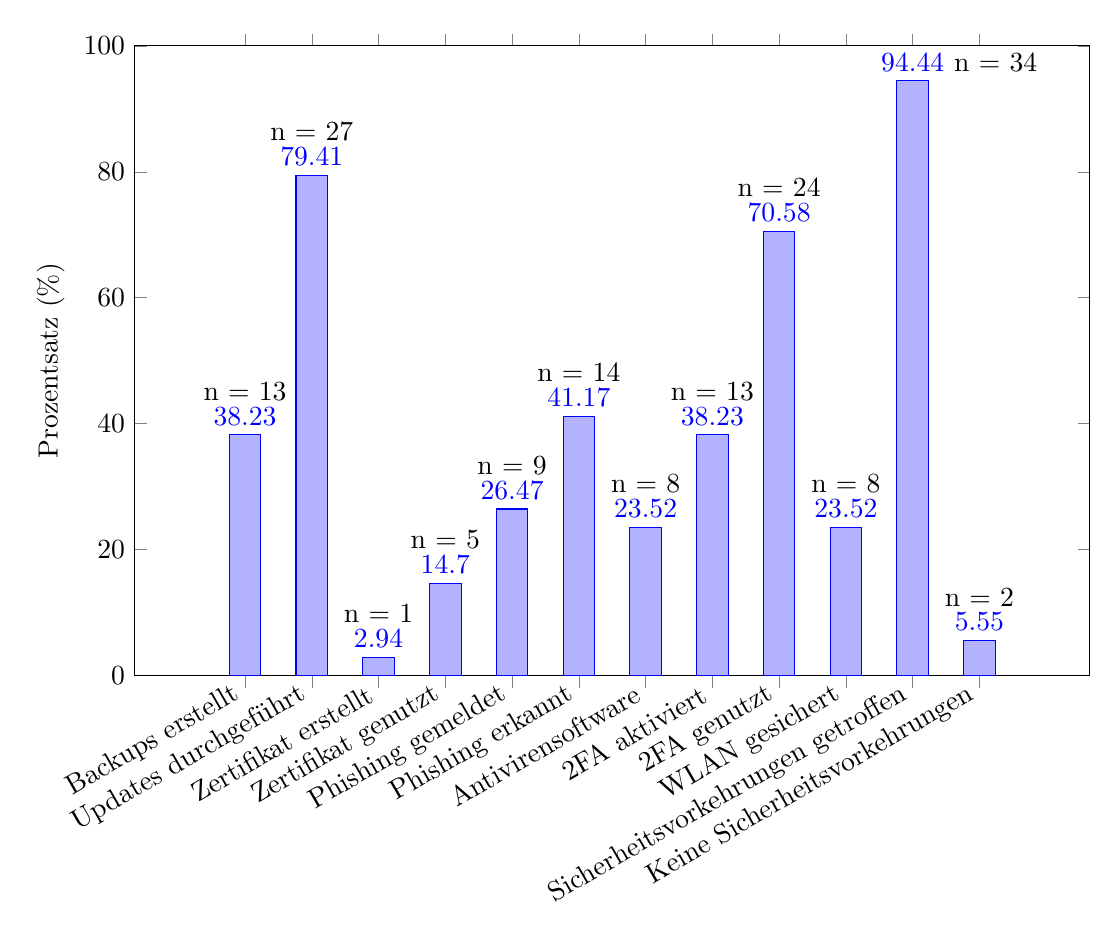
\begin{tikzpicture}
        \begin{axis}[
            ybar,
            symbolic x coords={Backups erstellt, Updates durchgeführt, Zertifikat erstellt, Zertifikat genutzt, Phishing gemeldet, Phishing erkannt, Antivirensoftware, 2FA aktiviert, 2FA genutzt, WLAN gesichert, Sicherheitsvorkehrungen getroffen, Keine Sicherheitsvorkehrungen},
            xtick=data,
            nodes near coords,
            xlabel=,
            ylabel=Prozentsatz (\%),
            x tick label style={rotate=30, anchor=east},
            ymin=0, ymax=100,
            enlarge x limits=0.15,
            width=\textwidth,
            height=8cm,
            scale only axis,
            bar width=0.4cm,
            every node near coord/.append style={anchor=south}, 
        ]
            \addplot coordinates {(Backups erstellt,38.23) (Updates durchgeführt,79.41) (Zertifikat erstellt,2.94) (Zertifikat genutzt,14.70) 
            (Phishing gemeldet,26.47) (Phishing erkannt,41.17) (Antivirensoftware,23.52) (2FA aktiviert,38.23) (2FA genutzt,70.58)
            (WLAN gesichert,23.52) (Sicherheitsvorkehrungen getroffen,94.44) (Keine Sicherheitsvorkehrungen,5.55)};

            \node[above=9pt] at (axis cs:Backups erstellt,38.23) {n = 13};
            \node[above=9pt] at (axis cs:Updates durchgeführt,79.41) {n = 27};
            \node[above=9pt] at (axis cs:Zertifikat erstellt,2.94) {n = 1};
            \node[above=9pt] at (axis cs:Zertifikat genutzt,14.70) {n = 5};
            \node[above=9pt] at (axis cs:Phishing gemeldet,26.47) {n = 9};
            \node[above=9pt] at (axis cs:Phishing erkannt,41.17) {n = 14};
            \node[above=9pt] at (axis cs:Antivirensoftware,23.52) {n = 8};
            \node[above=9pt] at (axis cs:2FA aktiviert,38.23) {n = 13};
            \node[above=9pt] at (axis cs:2FA genutzt,70.58) {n = 24};
            \node[above=9pt] at (axis cs:WLAN gesichert,23.52) {n = 8};
            \node[above=0pt, xshift=30pt] at (axis cs:Sicherheitsvorkehrungen getroffen,94.44) {n = 34};
            \node[above=9pt] at (axis cs:Keine Sicherheitsvorkehrungen,5.55) {n = 2};
        \end{axis}
    \end{tikzpicture}
    \caption{Sicherheitsvorkehrungen der Studierenden in den letzten vier Wochen vor Umfragebeginn, einschließlich derjenigen, die keine Vorkehrungen getroffen haben (n = 36)}
\end{figure}

Von den Befragten zeigen 58.33\% \((n = 21)\) Interesse an Schulungen, und 91.65\% \((n = 33)\) betonen die Wichtigkeit von IT-Sicherheit. Um Hilfe bei Problemen mit dem Computer, Laptop oder Smartphone zu bekommen verwendeten 91.66\% (\(n = 33\)) der Befragten, Suchmaschinen, während 36.11\% (\(n = 13\)) Freunde um Rat fragten. 13.88\% (\(n = 5\)) konsultierten die Familie, und 8.33\% (\(n = 3\)) suchten auf FAU-Seiten nach Informationen. Insgesamt kontaktierten 16.66\% \((n = 6)\) der Studierenden IT-Techniker, während ein Studierender Print-Publikationen nutzten. Es gab eine „Sonstige“-Antwort, die „BleepingComputer“ und „unix stackexchange“ erwähnte.\\
\\
75\% (\(n = 21\)) der Befragten nennen Prokrastination, 39.28\% (\(n = 11\)) Zeitmangel und 39.28\% (\(n = 11\)) Überforderung ihrer IT-Kenntnisse als Herausforderungen. 14.28\% (\(n = 4\)) der Befragten geben Angst oder Unsicherheit als Grund an. 30.55\% (\(n = 11\)) der Befragten berichten, dass sie selbst oder ein Familienmitglied bereits Opfer eines Cyberangriffs geworden sind.
\\
Die folgende Grafik zeigt die prozentuale und absolute Verteilung der häufigsten Hindernisse für die Umsetzung von IT-Sicherheitsmaßnahmen:

\begin{figure}[H]
\centering
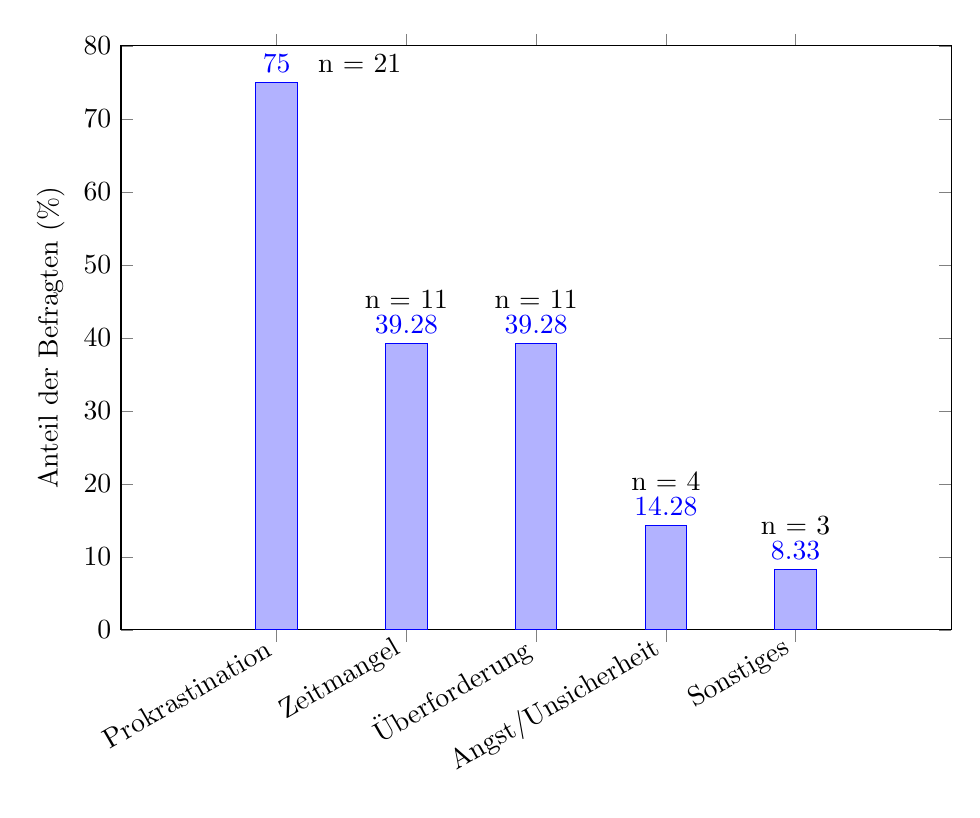
\begin{tikzpicture}
    \begin{axis}[
        ybar,
        symbolic x coords={Prokrastination, Zeitmangel, Überforderung, Angst/Unsicherheit, Sonstiges},
        xtick=data,
        ylabel={Anteil der Befragten (\%)},
        bar width=15pt,
        enlarge x limits=0.3,
        ymin=0,
        ymax=80,
        height=9cm,
        width=\textwidth,
        nodes near coords,
        nodes near coords align={vertical},
        x tick label style={rotate=30, anchor=east}
    ]
        \addplot coordinates {(Prokrastination,75) (Zeitmangel,39.28) (Überforderung,39.28) (Angst/Unsicherheit,14.28) (Sonstiges,8.33)};
        
        \node[above=0pt, xshift=30pt] at (axis cs:Prokrastination,75) {n = 21};
        \node[above=9pt] at (axis cs:Zeitmangel,39.28) {n = 11};
        \node[above=9pt] at (axis cs:Überforderung,39.28) {n = 11};
        \node[above=9pt] at (axis cs:Angst/Unsicherheit,14.28) {n = 4};
        \node[above=9pt] at (axis cs:Sonstiges,8.33) {n = 3};
    \end{axis}
\end{tikzpicture}
\caption{Hindernisse für die Umsetzung von IT-Sicherheitsmaßnahmen unter den Befragten (n = 36)}
\label{fig:hindernisse_it_sicherheit_balken}
\end{figure}
In der Kategorie „Sonstiges“ \(8.33\% \,(n = 3)\) wurden Gründe wie mangelnde Sorge über Sicherheitsrisiken genannt.\\
\\
Opfer eines Cyberangriffs wurden 30.55\% \((n = 11)\) der Befragten oder deren Familienmitglieder.\\
\\
Einen Mehrwert in den Fachschaften sehen 69.44\% \((n = 25)\) der Studierenden der Rechts- und Wirtschaftswissenschaftlichen Fakultät, während 30.56\% \((n = 11)\) diesen nicht erkennen.\\
\\
Die Unterstützung von Fachschaften bei IT-Problemen befürworten 69.44\% \((n = 25)\) der Studierenden der Rechts- und Wirtschaftswissenschaftlichen Fakultät.\\
\\
Die Webseite fau.info/infosec kannten 94.44\% \((n = 34)\) der Befragten nicht, während zwei Studierende sie kannten.

\textit{Hinweis: Die Angaben beziehen sich auf die Antworten im folgendem Abschnitt. Es handelt sich hierbei um ein Ranking, bei dem die Teilnehmer die Möglichkeit hatten, zwischen 2 und 7 Antworten auszuwählen. Daher kann es vorkommen, dass nicht alle Teilnehmer alle Fragen beantwortet haben und die Summe der Prozentsätze und der absoluten Anzahl möglicherweise nicht genau 100\% bzw. die Gesamtzahl der Teilnehmer ergibt.}

Von den Studierenden ordnen sich 36.11\% \((n = 13)\) der Aussage „Ich mag es, wenn alles geordnet und nach Plan läuft und mag keine Überraschungen“ zu. Zudem geben 19.44\% \((n = 7)\) der Studierenden an, „Ich liebe es, neue Dinge zu erleben und suche gerne Abenteuer“. Weiterhin ordnen sich 16.66\% \((n = 6)\) der Aussage „Ich möchte, dass sich alle gut verstehen und mag keine Streits“ zu. Weitere 13.88\% \((n = 5)\) ordnen sich der Aussage „Ich bin offen für neue Ideen und verschiedene Kulturen und mag Veränderungen“ zu. Spaß und Spannung suchen 8.33\% \((n = 3)\) der Studierenden und probieren gerne Neues aus. Schließlich ordnen sich zwei Studierende der Aussage „Ich suche Sicherheit und ein ruhiges Leben und meide Risiken“ zu.

\begin{figure}[H]
\centering
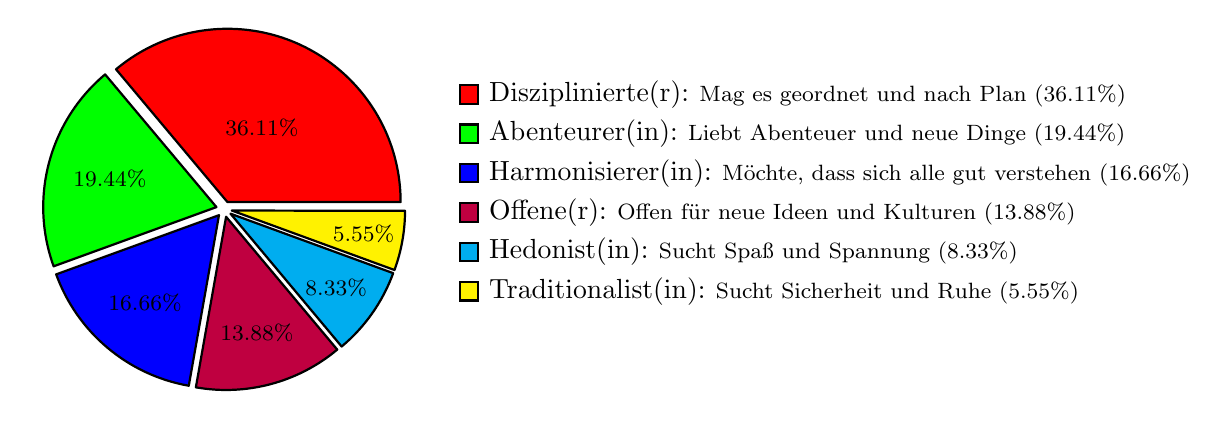
\begin{tikzpicture}
\pie[
    text=legend,
    radius=2.2,
    color={red, green, blue, purple, cyan, yellow},
    explode=0.1,
    before number=\footnotesize,
    after number=\%,
    text=legend
]{
    36.11/Disziplinierte(r): \newline \footnotesize{ Mag es geordnet und nach Plan (36.11\%)},
    19.44/Abenteurer(in): \newline \footnotesize{ Liebt Abenteuer und neue Dinge (19.44\%)},
    16.66/Harmonisierer(in): \newline \footnotesize{ Möchte, dass sich alle gut verstehen (16.66\%)},
    13.88/Offene(r): \newline \footnotesize{ Offen für neue Ideen und Kulturen (13.88\%)},
     8.33/Hedonist(in): \newline \footnotesize{ Sucht Spaß und Spannung (8.33\%)},
     5.55/Traditionalist(in): \newline \footnotesize{ Sucht Sicherheit und Ruhe (5.55\%)}
}
\end{tikzpicture}
\caption{Verteilung der Limbic Types \cite{hausel2011wissenschaftliche} unter Studierenden der Rechts- und Wirtschaftswissenschaftlichen Fakultät basierend auf ihren Aussagen (n = 36)}
\label{fig:limbic_types}
\end{figure}

\subsubsection{Offene Fragen - Rechts/Wirtschaftswissenschaftliche Fakultät}

\textbf{Q1: Welche Gedanken und Gefühle kommen dir in den Sinn, wenn du an IT-Sicherheit denkst?}

In Bezug auf IT-Sicherheit berichteten Studierende der Rechts- und Wirtschaftswissenschaftlichen Fakultät von Bewusstsein und Aufklärung (n = 3). Ein Studierender äußerte: „sehr sehr wichtig, sollte vor allem auch für die Generation unserer Eltern hervorgehoben und geschult werden.“ Ein weiterer Studierender erkannte: „Social Engineering --> Problem für große Organisationen.“

Frustration und Überforderung wurden ebenfalls genannt (n = 3). Ein Beispiel ist: „Das unangenehme Gefühl, dass ständig irgendwo meine Daten abgegriffen werden; damit der Druck, alle meine Konten besser schützen zu müssen und die Überforderung, weil ich nicht genau weiß, wie.“

Bedrohungen und Angst wurden von zwei Studierenden erwähnt. Ein Studierender meinte: „Gefahren, wichtige Informationen schützen.“ Ein weiterer betonte: „Firewall, ungutes Gefühl bei öffentlichem WLAN, ungutes Gefühl, wenn man auf Spotify oder Instagram regionale Werbung für deine Heimatstadt bekommt.“

Komplexität stellte für zwei Studierende ein Hindernis dar. Ein Studierender sagte: „Boah, zu kompliziert... meine Passwörter sorgen vor allem dafür, dass ich nicht mehr in meine Konten komme.“

Andere Themen, die von einzelnen Studierenden angesprochen wurden, waren Datenschutz/Überwachung (zweimal), und einmal jeweils Bequemlichkeit, Vertrauen in andere und Desinteresse.

\textbf{Q2: Aus welchen Gründen könntest du dich gegen die Anwendung bestimmter Sicherheitsmaßnahmen entscheiden und warum würdest du trotzdem auf IT-Sicherheit Wert legen?}

Das Sicherheitsbewusstsein führte dazu, dass Studierende Wert auf IT-Sicherheit legten, obwohl sie bestimmte Maßnahmen aufgrund ihrer Komplexität ablehnten (n = 5). Ein Studierender erklärte: „Zum Beispiel, 2FA ist irgendwie zu kompliziert, aber ich kümmere mich trotzdem um die Sicherheit meiner Passwörter.“

Bequemlichkeit und Usability wurden ebenfalls als Gründe genannt (n = 4). Ein Studierender äußerte: „Ehrlich gesagt ist es häufig aus Faulheit. Z.B. um ein neues sicheres Passwort für jedes Konto einzurichten, müsste ich einen Passwortmanager erstellen, was ich aber aus zeitlichen Gründen nicht mache.“

Zeitmangel und Aufwand waren weitere Faktoren (n = 3). Ein Studierender meinte: „Alles, was mir zu aufwendig erscheint, für einen eher geringen Gewinn. Die Relevanz der Daten ist entscheidend, d.h. bei Online-Banking betreibe ich einen viel größeren Aufwand als bei irgendeinem Gaming-Login.“

Jeweils ein Studierender nannte außerdem Kosten, mangelndes Wissen und die niedrige Relevanz der Daten als Gründe, bestimmte Sicherheitsmaßnahmen nicht zu implementieren.

\textbf{Q3: Kennst du deutsche Universitäten, Hochschulen oder öffentliche Einrichtungen, die aufgrund von Cyberangriffen temporär ihren Betrieb einstellen mussten?}

Acht Studierende der Rechts- und Wirtschaftswissenschaftlichen Fakultät berichteten, von solchen Vorfällen gehört zu haben (n = 8). Ein Studierender sagte: „Erst vor kurzem wieder eine Klinik in Deutschland.“ Ein anderer berichtete: „Hackerangriffe mit Erpressungsversuchen auf Krankenhäuser, man verlor Zugang zu Daten und musste dann versuchen mit Papier und Stift dagegenzuhalten.“

Vier Studierende erwähnten, dass diese Angriffe zu Einschränkungen von Diensten führten (n = 4). Ein Beispiel lautet: „Uni Köln... Irgendwas hat einfach ein paar Wochen nicht funktioniert.“

Zudem wurde auch von Datenverlust (n = 3) und zweimal von Erpressungsversuchen berichtet.

\textbf{Q4: Was waren die Folgen des Cyberangriffs? (Wenn die Frage bejaht wurde, dass in der Familie jemand Opfer eines Cyberangriffs wurde.)}

Zwei Studierende berichteten von Datenverlust oder -beschädigung. Ein Studierender sagte: „Ransomware auf dem PC. Das System musste neu aufgesetzt werden. Im Browser gespeicherte Passwörter wurden geklaut und mussten überall geändert werden.“

Finanzielle Schäden wurden ebenfalls genannt von zwei Studierenden genannt. So wurde berichtet: „Neue Geräte kaufen und alte Konten sperren lassen.“

Ein Studierender sprach von der Notwendigkeit einer Systemwiederherstellung, während ein anderer sagte, dass es keinen signifikanten Schaden gab.

\textbf{Q5: Aus welchen Gründen sollte die FAU der IT-Sicherheit eine hohe Priorität einräumen?}

Der Schutz sensibler Daten wurde von sechs Studierenden als Grund genannt (n = 6). Ein Studierender bemerkte: „Forschungsstandorte sind ein bevorzugtes Ziel von Angriffen. Außerdem stehen der Universität viele persönliche Daten der Studierenden zur Verfügung.“

Ein Studierender erwähnte auch die gesellschaftliche Verantwortung der FAU: „Weil die FAU die Verantwortung für sensible Daten einer sehr großen Studierendenschaft, Angestellten und anderen Stakeholders trägt.“

Ein weiterer Studierender nannte die Bedeutung der Verhinderung von Betriebsunterbrechungen.

\textbf{Q6: Gibt es Lehrstühle in deinem Fachbereich, die sich intensiv mit IT-Sicherheit beschäftigen? Falls ja, welche sind das und welche Maßnahmen ergreifen sie in diesem Bereich?}

Vier Studierende gaben an, keine Lehrstühle zu kennen, die sich intensiv mit IT-Sicherheit beschäftigen (n = 4). Ein Studierender äußerte: „Weiß ich nicht.“

Zwei Studierende nannten jedoch spezifische Lehrstühle oder Maßnahmen. Ein Beispiel lautet: „Ja, der Lehrstuhl 1 IT-Sicherheit. Ich kenne nur die angebotenen Module des Studiums.“

\textbf{Q7: An welchen Stellen auf den Webseiten der FAU suchst du typischerweise nach Informationen zur IT-Sicherheit?}

Zehn der Studierenden der Rechts- und Wirtschaftswissenschaftlichen Fakultät gaben an, keine spezifischen Informationen zur IT-Sicherheit auf den Webseiten der FAU zu suchen. Ein Studierender bemerkte: „Gar nicht.“ Ein anderer sagte: „Nie gesucht.“

Fünf Studierende nutzen das Rechenzentrum (n = 5), wie zum Beispiel: „Beim Rechenzentrum.“ Ein weiterer Studierender sagte, er suche auf „RRZE Seiten.“ nach Informationen.

\subsection{Technische Fakultät}

\subsubsection{Geschlossene Fragen - Technische Fakultät}

Die Studierenden der Technischen Fakultät haben im Durchschnitt 3 - 4 (\(3.44\)) Geräte pro Person. Von den Studierenden verwenden 70.58\% (\(n = 108\)) Windows, während 39.8\% (\(n = 61\)) Linux nutzen. macOS wird von 17.64\% (\(n = 27\)) der Befragten verwendet. Bei den Smartphones nutzen 64.05\% (\(n = 98\)) Android, und 37.25\% (\(n = 57\)) verwenden iOS. Jeweils ein Studierender verwendete CalyxOS, GrapheneOS und LineageOS als Smartphone-Betriebssystem.\\
\\
Von den Studierenden nutzen 74.82\% \((n = 104)\) FAU-eigene VPN-Dienste, und 72.72\% \((n = 104)\) verwenden private VPNs. Die VPN-Nutzung auf der Arbeit beträgt 51.04\% \((n = 77)\). \(2.72\% \,(n = 4)\), gaben an keinen VPN-Dienst zu nutzen.\\
Zusätzlich gaben zwei Personen an, einen eigenen VPN auf einem eigenen Server zu nutzen und eine Person gab an, den Ohm VPN zu nutzen.\\
\\
Von den Studierenden gaben 56.20\% \((n=86)\) an, für alle ihre Konten unterschiedliche Passwörter zu verwenden. Weitere 37.90\% \((n=58)\) nutzen für besonders wichtige Konten, wie etwa Online-Banking, spezifische Passwörter. Lediglich 5.88\% \((n=9)\) der Studierenden verwenden dasselbe Passwort für alle ihre Konten.\\
\\
Von den Befragten gaben 52.94\% \((n=81)\) an, ihre Passwörter auswendig zu kennen, während 19.60\% \((n=30)\) sie schriftlich festhalten. Darüber hinaus verwenden 58.82\% \((n=85)\) der Studierenden digitale Passwort-Manager, um ihre Zugangsdaten zu verwalten. Zudem speichern 9.15\% \((n=14)\) der Befragten ihre Passwörter digital, beispielsweise in Programmen wie Microsoft Word, während 90.84\% \((n=139)\) diese Methode nicht verwenden. Zusätzlich sichern 32.02\% \((n=49)\) der Befragten ihre Passwörter im Browser.\\
Ein Studierender gab an „I decipher my password. I just write 2-3digitz somewhere“\\
\\
Die folgenden Angaben beziehen sich auf die von den Studierenden in den letzten vier Wochen vor Umfragebeginn getroffenen Sicherheitsvorkehrungen: 50.68\% der Befragten, die Sicherheitsvorkehrungen getroffen haben (\(n = 146\)), gaben an, regelmäßig Backups zu erstellen, und 89.04\% (\(n = 130\)) führen regelmäßig Updates durch. 5.47\% (\(n = 8\)) der Befragten haben in diesem Zeitraum ein E-Mail-Zertifikat erstellt, und 12.32\% (\(n = 18\)) haben ein solches Zertifikat genutzt. 46.57\% (\(n = 68\)) der Befragten erkannten Phishing-Versuche, und 16.43\% (\(n = 24\)) haben diese Vorfälle gemeldet.\\
\\
79.45\% (\(n = 116\)) der Befragten in der technischen Fakultät gaben an, keine Antivirensoftware zu verwenden, während 20.54\% (\(n = 30\)) dies tun. 76.71\% (\(n = 112\)) haben 2FA (Zwei-Faktor-Authentifizierung) nicht aktiviert, während 23.28\% (\(n = 34\)) dies getan haben. 78.76\% (\(n = 115\)) der Befragten gaben an, 2FA zu nutzen, während 21.23\% (\(n = 31\)) diese Sicherheitsmaßnahme nicht verwenden.\\
\\
88.35\% der Befragten (\(n = 129\)) gaben an, ihr WLAN nicht gesichert zu haben, während 11.64\% (\(n = 17\)) dies getan haben. Schließlich erklärten 95.42\% (\(n = 146\)), dass sie Sicherheitsvorkehrungen getroffen haben, während 4.58\% (\(n = 7\)) angaben, keine solchen Vorkehrungen getroffen zu haben.\\
\\
Die folgende Grafik zeigt die prozentuale und absolute Verteilung der von den Studierenden in den letzten vier Wochen vor Umfragebeginn getroffenen Sicherheitsvorkehrungen in der technischen Fakultät:

\begin{figure}[H]
    \centering
    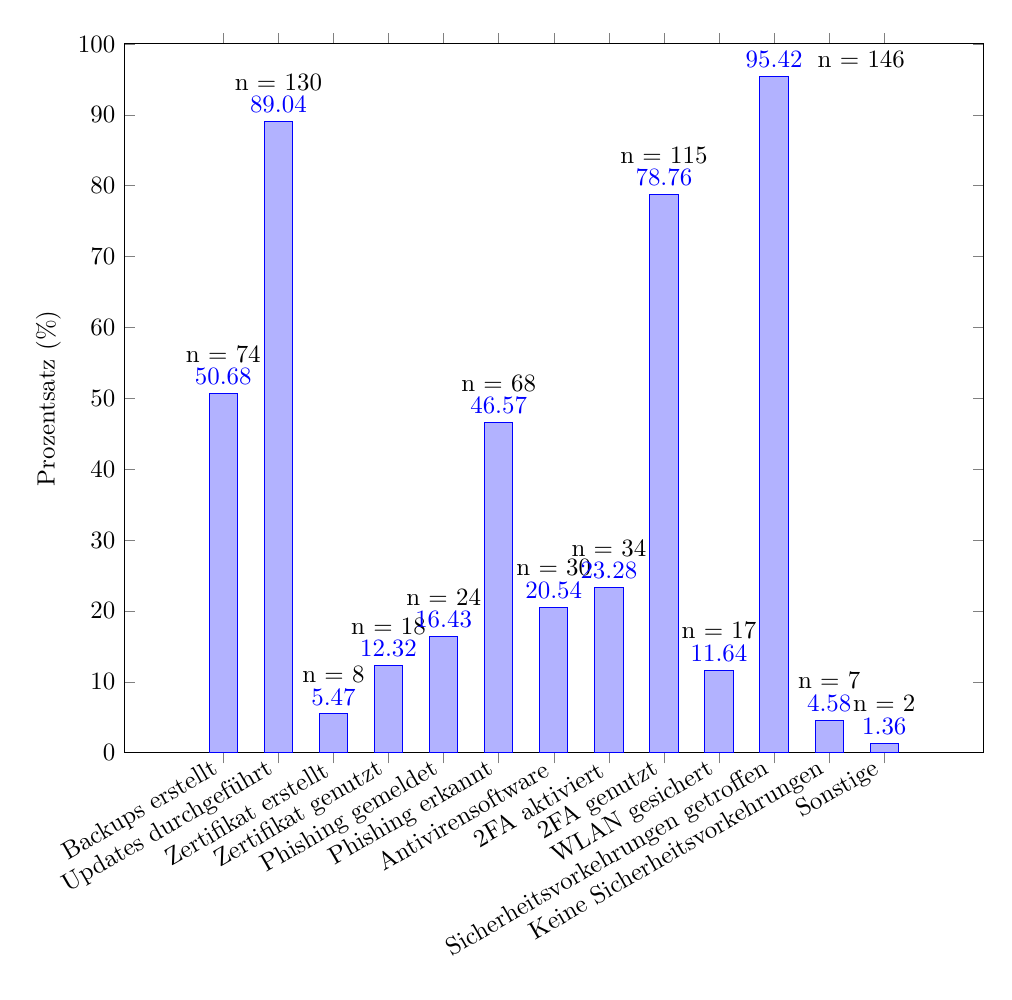
\begin{tikzpicture}[scale=0.9]
        \begin{axis}[
            ybar,
            symbolic x coords={Backups erstellt, Updates durchgeführt, Zertifikat erstellt, Zertifikat genutzt, Phishing gemeldet, Phishing erkannt, Antivirensoftware, 2FA aktiviert, 2FA genutzt, WLAN gesichert, Sicherheitsvorkehrungen getroffen, Keine Sicherheitsvorkehrungen, Sonstige},
            xtick=data,
            nodes near coords,
            ylabel=Prozentsatz (\%),
            x tick label style={rotate=30, anchor=east},
            ymin=0, ymax=100,
            enlarge x limits=0.15,
            width=\textwidth,
            height=10.0cm,
            scale only axis,
            bar width=0.4cm,
            every node near coord/.append style={anchor=south}
        ]
            \addplot coordinates {(Backups erstellt,50.68) (Updates durchgeführt,89.04) (Zertifikat erstellt,5.47) (Zertifikat genutzt,12.32) 
            (Phishing gemeldet,16.43) (Phishing erkannt,46.57) (Antivirensoftware,20.54) (2FA aktiviert,23.28) (2FA genutzt,78.76)
            (WLAN gesichert,11.64) (Sicherheitsvorkehrungen getroffen,95.42) (Keine Sicherheitsvorkehrungen,4.58) (Sonstige,1.36)};
            
            \node[above=9pt] at (axis cs:Backups erstellt,50.68) {n = 74};
            \node[above=9pt] at (axis cs:Updates durchgeführt,89.04) {n = 130};
            \node[above=9pt] at (axis cs:Zertifikat erstellt,5.47) {n = 8};
            \node[above=9pt] at (axis cs:Zertifikat genutzt,12.32) {n = 18};
            \node[above=9pt] at (axis cs:Phishing gemeldet,16.43) {n = 24};
            \node[above=9pt] at (axis cs:Phishing erkannt,46.57) {n = 68};
            \node[above=9pt] at (axis cs:Antivirensoftware,20.54) {n = 30};
            \node[above=9pt] at (axis cs:2FA aktiviert,23.28) {n = 34};
            \node[above=9pt] at (axis cs:2FA genutzt,78.76) {n = 115};
            \node[above=9pt] at (axis cs:WLAN gesichert,11.64) {n = 17};
            \node[above=0pt, xshift=35pt] at (axis cs:Sicherheitsvorkehrungen getroffen,95.42) {n = 146};
            \node[above=9pt] at (axis cs:Keine Sicherheitsvorkehrungen,4.58) {n = 7};
            \node[above=9pt] at (axis cs:Sonstige,1.36) {n = 2};
        \end{axis}
    \end{tikzpicture}
    \caption{Sicherheitsvorkehrungen der Studierenden der Technischen Fakultät in den letzten vier Wochen vor Umfragebeginn, einschließlich derjenigen, die keine Vorkehrungen getroffen haben (n = 153)}
\end{figure}

Unter „Sonstige“ haben zwei Studierende folgende Antworten gegeben: einer gab an, „Plausibilitätsprüfungen von Links und E-Mails“ durchzuführen, und ebenfalls ein anderer erwähnte „Vollfestplattenverschlüsselung, Unattended-Upgrades, keine exim4, keine Usernamespaces und SSH nur mit Keys“.\\
\\
Von den Befragten zeigen 54.24\% \((n = 83)\) Interesse an Schulungen, und 98.03\% \((n = 150)\) betonen die Wichtigkeit von IT-Sicherheit.\\
\\
Um Hilfe bei Problemen mit dem Computer, Laptop oder Smartphone zu bekommen verwendeten 98.69\% (\(n = 151\)) der Befragten Suchmaschinen, 47.71\% (\(n = 73\)) suchten Rat bei Freunden, und 15.68\% (\(n = 24\)) konsultierten die Familie. FAU-Seiten wurden von 13.72\% (\(n = 21\)) genutzt, während 16.33\% (\(n = 25\)) IT-Techniker kontaktierten. Zwei Studierende gaben an gaben an, Print-Publikationen zu verwenden. Zudem wurden n = 6 (3.92\%) „Sonstige“-Antworten angegeben, darunter „mac Support von der FAU“, „reddit“ und „GPT-4o“.\\
\\
74.10\% (\(n = 103\)) der Befragten nennen Prokrastination, 50.35\% (\(n = 70\)) Zeitmangel und 23.02\% (\(n = 32\)) Überforderung ihrer IT-Kenntnisse als Herausforderungen für die Anwendung von IT-Sicherheitsmaßnahmen. 8.63\% (\(n = 12\)) der Befragten haben Angst oder Unsicherheit als Grund angegeben.\\
\\
Die folgende Grafik zeigt die prozentuale und absolute Verteilung der häufigsten Hindernisse für die Umsetzung von IT-Sicherheitsmaßnahmen:

\begin{figure}[H]
\centering
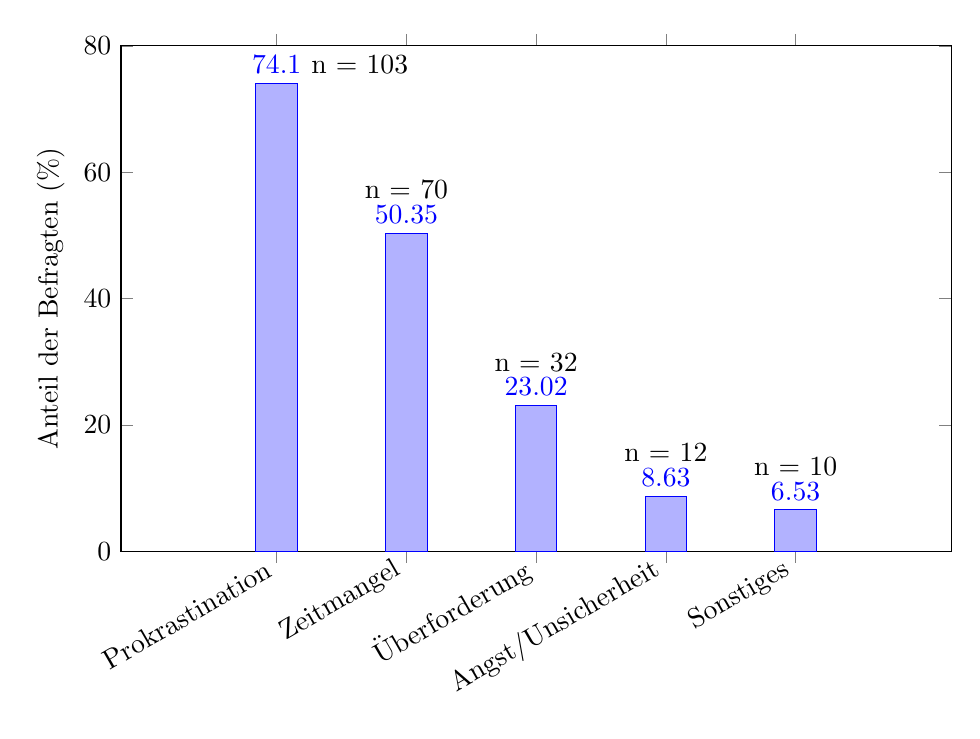
\begin{tikzpicture}
    \begin{axis}[
        ybar,
        symbolic x coords={Prokrastination, Zeitmangel, Überforderung, Angst/Unsicherheit, Sonstiges},
        xtick=data,
        ylabel={Anteil der Befragten (\%)},
        bar width=15pt,
        enlarge x limits=0.3,
        ymin=0,
        ymax=80,
        height=8cm,
        width=\textwidth,
        nodes near coords,
        nodes near coords align={vertical},
        x tick label style={rotate=30, anchor=east}
    ]
        \addplot coordinates {(Prokrastination,74.10) (Zeitmangel,50.35) (Überforderung,23.02) (Angst/Unsicherheit,8.63) (Sonstiges,6.53)};
        
        \node[above=0pt, xshift=30pt] at (axis cs:Prokrastination,74.10) {n = 103};
        \node[above=9pt] at (axis cs:Zeitmangel,50.35) {n = 70};
        \node[above=9pt] at (axis cs:Überforderung,23.02) {n = 32};
        \node[above=9pt] at (axis cs:Angst/Unsicherheit,8.63) {n = 12};
        \node[above=9pt] at (axis cs:Sonstiges,6.53) {n = 10};
    \end{axis}
\end{tikzpicture}
\caption{Hindernisse für die Umsetzung von IT-Sicherheitsmaßnahmen unter den Befragten (n = 153)}
\label{fig:hindernisse_it_sicherheit_balken}
\end{figure}

In der Kategorie „Sonstiges“ wurden verschiedene Gründe genannt, darunter die Kosten für VPNs und Backups, und die Unsicherheit bezüglich der Informationsqualität \(6.53\% \,(n = 10)\).\\
\\
Opfer eines Cyberangriffs geworden sind 27.45\% \((n = 42)\) der Befragten.\\
\\
Einen Mehrwert in den Fachschaften sehen 72.54\% \((n = 111)\) der Studierenden der Technischen Fakultät, während 27.45\% \((n = 42)\) diesen nicht erkennen.\\
\\
Die Unterstützung von Fachschaften bei IT-Problemen befürworten 77.12\% \((n = 118)\) der Studierenden der Technischen Fakultät.\\
\\
Die Webseite fau.info/infosec kannten 92.15\% \((n = 141)\) der Befragten nicht, während 7.84\% \((n = 12)\) sie kannten.

\textit{Hinweis: Die Angaben beziehen sich auf die Antworten im folgendem Abschnitt. Es handelt sich hierbei um ein Ranking, bei dem die Teilnehmer die Möglichkeit hatten, zwischen 2 und 7 Antworten auszuwählen. Daher kann es vorkommen, dass nicht alle Teilnehmer alle Fragen beantwortet haben und die Summe der Prozentsätze und der absoluten Anzahl möglicherweise nicht genau 100\% bzw. die Gesamtzahl der Teilnehmer ergibt.}

Von den Studierenden ordnen sich 23.52\% \((n = 36)\) der Aussage „Ich mag es, wenn alles geordnet und nach Plan läuft und mag keine Überraschungen“ zu. Zudem geben 18.95\% \((n = 29)\) der Studierenden an, „Ich liebe es, neue Dinge zu erleben und suche gerne Abenteuer“. Weiterhin ordnen sich 18.30\% \((n = 28)\) der Aussage „Ich möchte, dass sich alle gut verstehen und mag keine Streits“ zu. Der Aussage „Ich bin offen für neue Ideen und verschiedene Kulturen und mag Veränderungen“ ordnen sich 15.03\% \((n = 23)\) der Studierenden zu. Sicherheit und ein ruhiges Leben suchen 11.11\% \((n = 17)\) der Studierenden und meiden Risiken. Ebenfalls 11.11\% \((n = 17)\) ordnen sich der Aussage „Ich suche nach Spaß und Spannung und probiere gerne Neues aus“ zu. Schließlich geben 1.96\% \((n = 3)\) der Studierenden an, „Ich möchte gerne führen und entscheiden und stehe gerne im Mittelpunkt“.

\begin{figure}[H]
\centering
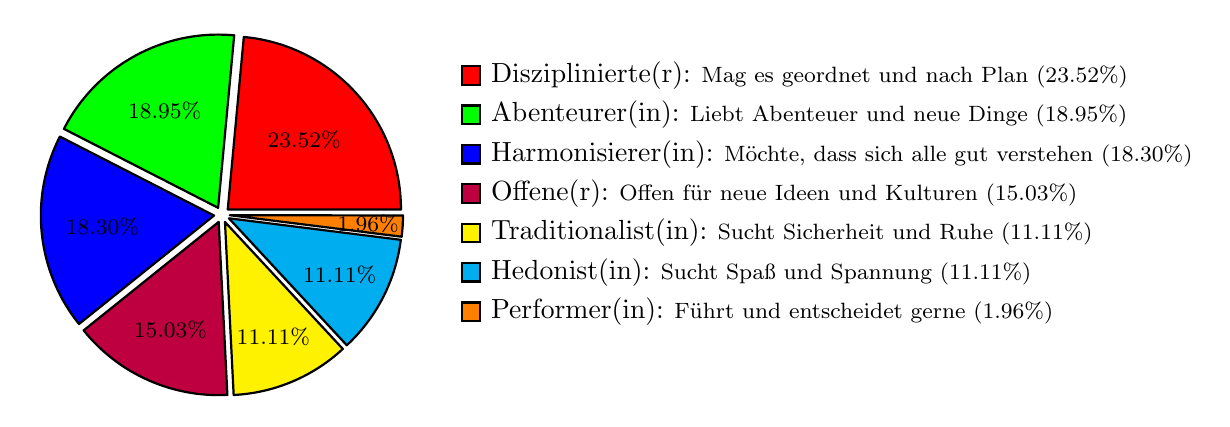
\begin{tikzpicture}
\pie[
    text=legend,
    radius=2.2,
    color={red, green, blue, purple, yellow, cyan, orange},
    explode=0.1,
    before number=\footnotesize,
    after number=\%,
    text=legend
]{
    23.52/Disziplinierte(r): \newline \footnotesize{ Mag es geordnet und nach Plan (23.52\%)},
    18.95/Abenteurer(in): \newline \footnotesize{ Liebt Abenteuer und neue Dinge (18.95\%)},
    18.30/Harmonisierer(in): \newline \footnotesize{ Möchte, dass sich alle gut verstehen (18.30\%)},
    15.03/Offene(r): \newline \footnotesize{ Offen für neue Ideen und Kulturen (15.03\%)},
    11.11/Traditionalist(in): \newline \footnotesize{ Sucht Sicherheit und Ruhe (11.11\%)},
    11.11/Hedonist(in): \newline \footnotesize{ Sucht Spaß und Spannung (11.11\%)},
     1.96/Performer(in): \newline \footnotesize{ Führt und entscheidet gerne (1.96\%)}
}
\end{tikzpicture}
\caption{Verteilung der Limbic Types \cite{hausel2011wissenschaftliche} unter den Studierenden der Technischen Fakultät basierend auf ihren Aussagen (n = 153)}
\label{fig:limbic_types}
\end{figure}

\subsubsection{Offene Fragen - Technische Fakultät}

\textbf{Q1: Welche Gedanken und Gefühle kommen dir in den Sinn, wenn du an IT-Sicherheit denkst?}

In Bezug auf IT-Sicherheit berichteten die Studierenden der Technischen Fakultät häufig über die Wichtigkeit und Notwendigkeit von IT-Sicherheitsmaßnahmen (n = 22). Ein Studierender betonte: „IT-Sicherheit ist extrem wichtig, um sensible Daten vor unbefugtem Zugriff zu schützen.“ Ein weiterer Studierender erwähnte: „Ohne IT-Sicherheit könnten wichtige Forschungsdaten in die falschen Hände geraten.“

Frustration und Überforderung wurden ebenfalls häufig genannt (n = 13). Ein Beispiel dafür ist die Aussage: „Die ständigen Anforderungen an die IT-Sicherheit überfordern mich, es ist schwer, alles im Blick zu behalten.“ Ein anderer Studierender erwähnte: „Die Komplexität der IT-Sicherheit macht es oft schwierig, alle Maßnahmen umzusetzen.“

Mehrere Studierende äußerten Bedrohungen und Angst im Zusammenhang mit IT-Sicherheit (n = 10). Ein Studierender meinte: „Ich habe Angst, dass meine persönlichen Daten gestohlen werden könnten.“ Ein anderer Studierender schrieb: „Hackerangriffe auf meine Accounts bereiten mir große Sorgen.“

Auch Praktische Maßnahmen wurden von eingie Studierenden erwähnt (n = 9). Ein Studierender sagte: „Ich versuche, regelmäßig Backups zu machen, um meine Daten zu schützen.“ Ein weiterer Studierender erklärte: „Die Nutzung eines Passwortmanagers hat meine Sicherheit erhöht.“

\textbf{Q2: Aus welchen Gründen könntest du dich gegen die Anwendung bestimmter Sicherheitsmaßnahmen entscheiden und warum würdest du trotzdem auf IT-Sicherheit Wert legen?}

Bequemlichkeit und Usability wurden häufig als Gründe genannt, Sicherheitsmaßnahmen nicht umzusetzen (n = 27). Ein Studierender sagte: „Zwei-Faktor-Authentifizierung ist zu umständlich, vor allem im Alltag.“ Ein anderer bemerkte: „Die Sicherheitseinstellungen sind oft so kompliziert, dass ich sie nicht immer nutze.“

Wegen ihres Sicherheitsbewusstseins legten die Studierenden großen Wert auf IT-Sicherheit, lehnten jedoch bestimmte Maßnahmen aufgrund ihrer Unannehmlichkeiten ab (n = 25). Ein Studierender erklärte: „Auch wenn es lästig ist, weiß ich, dass IT-Sicherheit wichtig ist, um meine Daten zu schützen.“ Ein anderer meinte: „Trotz der Umständlichkeit achte ich auf die Sicherheit meiner Systeme.“

Zeitmangel und Aufwand wurden ebenfalls als Barrieren genannt (n = 18). Ein Studierender äußerte: „Die Implementierung von Sicherheitsmaßnahmen ist oft sehr zeitaufwendig.“ Ein anderer erklärte: „Die Wartung meiner Sicherheitsvorkehrungen kostet mich viel Zeit, die ich nicht immer habe.“

\textbf{Q3: Kennst du deutsche Universitäten, Hochschulen oder öffentliche Einrichtungen, die aufgrund von Cyberangriffen temporär ihren Betrieb einstellen mussten?}

Viele Studierende der Technischen Fakultät berichteten, von solchen Vorfällen gehört zu haben (n = 63). Ein Studierender sagte: „Ich habe von mehreren Universitäten gehört, die nach Cyberangriffen ihren Betrieb einstellen mussten.“ Ein anderer Studierender erklärte: „An der TH Nürnberg gab es nach einem Angriff für Wochen kein funktionierendes VPN.“

Mehrere Studierende berichteten, dass diese Angriffe zu Einschränkungen von Diensten führten (n = 22). Ein Beispiel lautet: „Nach einem Angriff konnten wir uns nicht mehr in das Hochschulnetzwerk einloggen.“ Ein weiteres Beispiel beschreibt den Ausfall von Diensten: „Die E-Mail-Dienste der Hochschule waren nach einem Cyberangriff für mehrere Tage offline.“

Einige Studierende erwähnten auch Erpressung (n = 6) und Einstellung des Betriebs (n = 4). Ein Studierender sagte: „Eine Universität musste ihren gesamten Betrieb nach einem Angriff einstellen.“ Ein Weiterer berichtete: „Die Angreifer forderten Lösegeld, um die Systeme wieder freizugeben.“

\textbf{Q4: Was waren die Folgen des Cyberangriffs? (Wenn die Frage bejaht wurde, dass in der Familie jemand Opfer eines Cyberangriffs wurde.)}

Einige Studierende berichteten von keinen signifikanten Schäden (n = 12). Ein Studierender erklärte: „Es gab keine größeren Schäden, aber die Sicherheitssysteme mussten verstärkt werden.“ Ein weiterer berichtete: „Mein Konto wurde gesperrt, aber der Schaden konnte schnell behoben werden.“

Finanzielle Schäden wurden ebenfalls mehrfach erwähnt (n = 9). Ein Studierender sagte: „Loss of an adequate amount of money.“ Ein anderer Studierender berichtete: „Ein Cyberangriff führte dazu, dass ich Geld verlor, das ich nicht wiederbekam.“

Ein weiterer Effekt war der Verlust des Kontos oder Zugangs (n = 9). Ein Studierender sagte: „Ich habe den Zugang zu meinem Social-Media-Account verloren.“ Ein anderer erklärte: „Mein Konto wurde gehackt und ich musste es komplett wiederherstellen.“

\textbf{Q5: Aus welchen Gründen sollte die FAU der IT-Sicherheit eine hohe Priorität einräumen?}

Der Schutz sensibler Daten wurde von den vielen Studierenden als Grund genannt (n = 40). Ein Studierender sagte: „Die Universität speichert viele persönliche Daten, die geschützt werden müssen.“ Ein anderer schrieb: „Forschungsergebnisse sind oft vertraulich und müssen vor Cyberangriffen geschützt werden.“

Ein weiterer wichtiger Grund war die Verhinderung von Betriebsunterbrechungen (n = 15). Ein Studierender äußerte: „IT-Sicherheit ist wichtig, um den Betrieb der Universität aufrechtzuerhalten.“ Ein anderer schrieb: „Ein Angriff könnte den Betrieb der Hochschule für Wochen lahmlegen.“

Auch die Reputation und Professionalität der Universität wurden mehrfach genannt (n = 8). Ein Studierender bemerkte: „Eine Hochschule muss sicherstellen, dass sie ihren Ruf durch angemessene Sicherheitsmaßnahmen schützt.“ Ein anderer ergänzte: „IT-Sicherheit ist ein Zeichen von Professionalität und sollte entsprechend behandelt werden.“

\textbf{Q6: Gibt es Lehrstühle in deinem Fachbereich, die sich intensiv mit IT-Sicherheit beschäftigen? Falls ja, welche sind das und welche Maßnahmen ergreifen sie in diesem Bereich?}

Viele Studierende gaben an, keine Lehrstühle zu kennen, die sich intensiv mit IT-Sicherheit beschäftigen (n = 32). Ein Studierender äußerte: „Ich wüsste nicht, dass es einen Lehrstuhl für IT-Sicherheit gibt.“ Ein anderer sagte: „In meinem Bereich wird das Thema IT-Sicherheit kaum angesprochen.“

Einige Studierende nannten jedoch den Informatik Lehrstuhl 1 als bekannt für IT-Sicherheitsforschung (n = 26). Ein Studierender sagte: „Der Lehrstuhl für Informatik 1 beschäftigt sich intensiv mit IT-Sicherheit.“ Ein Anderer erklärte: „Dort gibt es Vorlesungen und Projekte zur IT-Sicherheit.“

\textbf{Q7: An welchen Stellen auf den Webseiten der FAU suchst du typischerweise nach Informationen zur IT-Sicherheit?}

Die Mehrheit der Studierenden der Technischen Fakultät gab an, keine Informationen zur IT-Sicherheit auf den Webseiten der FAU zu suchen (n = 29). Ein Studierender gab an er nutze die FAU-Seiten „Gar nicht“,  ein anderer bemerkte: „Ich habe noch nie nach Informationen zur IT-Sicherheit auf den Webseiten der FAU gesucht.“

Einige Studierende suchen nach Informationen im Rechenzentrum (n = 16). Ein Studierender erwähnte: „Auf Seiten des RRZE.“ Ein anderer sagte er nutze die Seite „rrze.fau.de.“

Zwei Studierende gaben an, E-Mails als Informationsquelle zu nutzen. Einer von ihnen sagte: „Nicht. Höchstens per Newsletter.“

Zwei Studierenden nannte den Lehrstuhl I1 als Quelle erwähnt wurde: „Lehrstuhl für Informatik 1, IT-Sicherheitsinfrastrukturen.“

\subsection{Vergleich der Limbic Types der Studierenden pro Fakultät}

Die verschiedenen Limbic Types \cite{hausel2011wissenschaftliche} der Studierenden geben Einblicke in deren Verhalten, Motivation und Präferenzen im Zusammenhang mit IT-Sicherheitsmaßnahmen. Jeder Limbic Type weist unterschiedliche Merkmale und Herangehensweisen auf, die im Kontext der Entwicklung von Awareness-Kampagnen relevant sein könnten. Im Folgenden werden die Hauptmerkmale der Limbic Types der verschiedenen Studierendengruppen dargestellt und miteinander verglichen, um ein besseres Verständnis der unterschiedlichen Verhaltensweisen und Präferenzen zu gewinnen.

\begin{table}[H]
\centering
\resizebox{\textwidth}{!}{%
\begin{tabular}{|p{4.3cm}|p{2.6cm}|p{2.9cm}|p{2.5cm}|p{1.4cm}|p{2.7cm}|p{1.9cm}|p{2cm}|}
\hline
\textbf{Fakultät} & \textbf{\large Disziplinierte} & \textbf{\large Harmonisierer} & \textbf{\large Abenteurer} & \textbf{\large Offene} & \textbf{\large Traditionalist} & \textbf{\large Hedonist} & \textbf{\large Performer} \\ \hline
\textbf{Medizinische Fakultät} & \large 28\% & \large 28\% & \large 20\% & \large 4\% & \large 12\% & \large 4\% & \large 4\% \\ \hline
\textbf{Naturwissenschaftliche Fakultät} & \large 35.55\% & \large 15.55\% & \large 20\% & \large 17.77\% & \large 2.22\% & \large 6.66\% & \large 2.22\% \\ \hline
\textbf{Philosophische Fakultät} & \large 19.44\% & \large 16.66\% & \large 8.33\% & \large 30.55\% & \large 19.44\% & \large 5.55\% & \large 0.00\% \\ \hline
\textbf{Rechts- und Wirtschaftswissenschaftliche Fakultät} & \large 36.11\% & \large 16.66\% & \large 19.44\% & \large 13.88\% & \large 5.55\% & \large 8.33\% & \large 0.00\% \\ \hline
\textbf{Technische Fakultät} & \large 23.52\% & \large 18.30\% & \large 18.95\% & \large 15.03\% & \large 11.11\% & \large 11.11\% & \large 1.96\% \\ \hline
\end{tabular}%
}
\caption{Vergleich der Limbic Types nach Fakultäten}
\end{table}

Die \textbf{Disziplinierten}, die stark auf Ordnung und Struktur setzen, sind in der Rechts- und Wirtschaftswissenschaftlichen Fakultät (36.11\%) sowie der Naturwissenschaftlichen Fakultät (35.55\%) am häufigsten vertreten. Im Gegensatz dazu ist ihr Anteil in der Philosophischen Fakultät mit 19.44\% am geringsten. Der höhere Anteil der Disziplinierten in der Rechts- und Wirtschaftswissenschaftlichen sowie der Naturwissenschaftlichen Fakultät spiegelt möglicherweise strukturelle Unterschiede in den Präferenzen oder Anforderungen wider.

Die \textbf{Harmonisierer}, die Wert auf ein konfliktfreies Umfeld legen, sind in der Medizinischen Fakultät mit 28\% stark vertreten. Ein hoher Anteil der Harmonisierer in der Medizinischen Fakultät könnte darauf hindeuten, dass Zusammenarbeit und ein harmonisches Umfeld hier hier besonders wichtig sind. In den anderen Fakultäten ist der Anteil der Harmonisierer niedriger, insbesondere in der Naturwissenschaftlichen Fakultät (15.55\%) und der Rechts- und Wirtschaftswissenschaftlichen Fakultät (16.66\%).

Der Anteil der \textbf{Abenteurer}, die gerne neue Dinge ausprobieren und nach Abenteuern suchen, ist in allen Fakultäten relativ konstant und bewegt sich um die 20\%-Marke, mit einer Ausnahme in der Philosophischen Fakultät, wo dieser Anteil nur 8.33\% beträgt. Der geringere Anteil der Abenteurer in der Philosophischen Fakultät könnte darauf hinweisen, dass Studierende in dieser Fakultät weniger risikofreudig sind.

Studierende, die sich den \textbf{Offenen} zuordnen, sind besonders stark in der Philosophischen Fakultät vertreten, wo 30.55\% sich diesem Typ zuordnen. Der hohe Anteil der Offenen in der Philosophischen Fakultät könnte ein Hinweis darauf sein, dass Studierende hier besonders offen für neue Ideen und Kulturen sind. In der Medizinischen Fakultät hingegen ist der Anteil der Offenen mit 4\% am niedrigsten.

Der Anteil der \textbf{Traditionalisten}, die Sicherheit und ein ruhiges Leben bevorzugen, ist in der Medizinischen Fakultät (12\%) und der Technischen Fakultät (11.11\%) vergleichsweise hoch, während in der Naturwissenschaftlichen Fakultät der geringste Anteil zu finden ist (2.22\%). Der höhere Anteil der Traditionalisten in der Medizinischen und Technischen Fakultät könnte darauf hinweisen, dass Stabilität und Sicherheit hier eine größere Rolle spielen.

Der Anteil der \textbf{Hedonisten}, die nach Spaß und Spannung suchen, ist in der Technischen Fakultät mit 11.11\% am höchsten, gefolgt von der Rechts- und Wirtschaftswissenschaftlichen Fakultät (8.33\%). In der Medizinischen Fakultät und der Philosophischen Fakultät sind Hedonisten mit nur 4\% bzw. 5.55\% seltener vertreten. Diese Verteilung könnte auf unterschiedliche Präferenzen der Studierenden hinsichtlich Spaß, Spannung und risikoreichem Verhalten hinweisen.

Die \textbf{Performer}, die gerne führen und entscheiden, treten in den meisten Fakultäten kaum oder gar nicht auf. In der Medizinischen Fakultät und Naturwissenschaftlichen Fakultät finden sich geringe Anteile (4\% bzw. 2.22\%), während in der Philosophischen Fakultät und der Rechts- und Wirtschaftswissenschaftlichen Fakultät keine Performer-Typen vertreten sind. Diese geringe Präsenz könnte auf eine tendenziell zurückhaltendere Haltung in Entscheidungssituationen innerhalb der Studierendenschaft hinweisen.

Die folgende Abbildung zeigt den prozentualen Vergleich der Limbic Types der Studierenden pro Fakultät. Die Werte sind gestapelt, um die Verteilung der verschiedenen Typen in den Fakultäten besser zu visualisieren:

\begin{figure}[H]
\centering
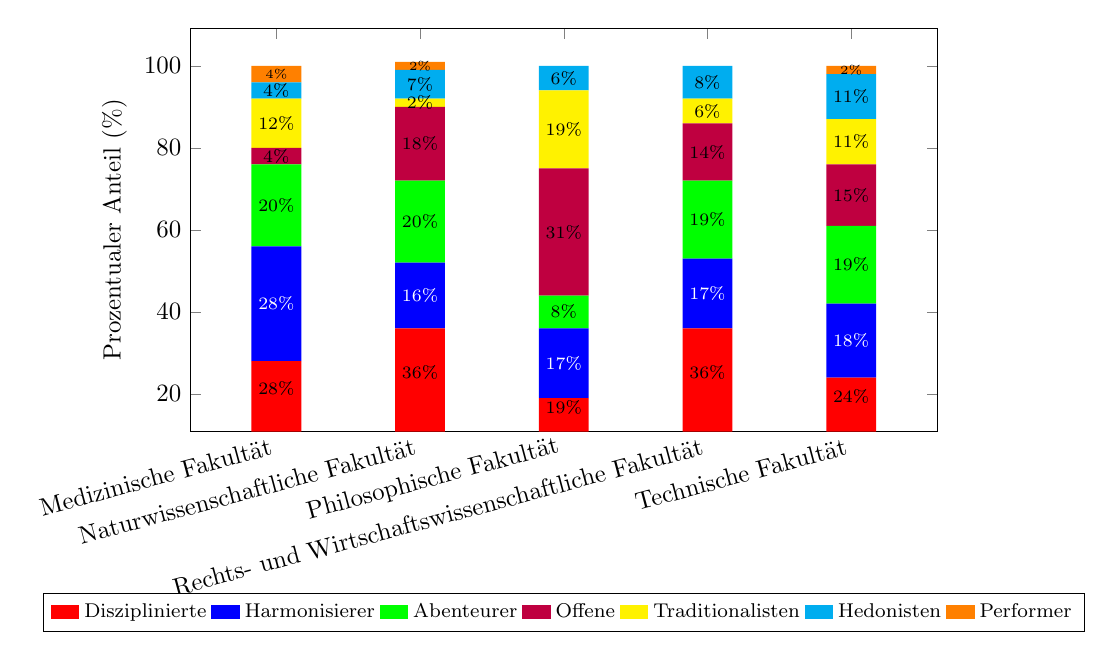
\begin{tikzpicture}[scale=0.9]
    \begin{axis}[
        ybar stacked,
        bar width=20pt,
        width=1.0\textwidth,
        height=0.6\textwidth,
        enlarge x limits=0.15,
        ylabel={Prozentualer Anteil (\%)},
        symbolic x coords={
            Medizinische Fakultät,
            Naturwissenschaftliche Fakultät,
            Philosophische Fakultät,
            Rechts- und Wirtschaftswissenschaftliche Fakultät,
            Technische Fakultät
        },
        xtick=data,
        x tick label style={rotate=15, anchor=east, yshift=-5pt},
        legend style={
            at={(0.5,-0.4)},
            anchor=north,
            legend columns=7,
            font=\footnotesize
        },
        bar shift=0pt,
        draw=none,
        legend image code/.code={%
            \draw[draw=none] (0cm,-0.1cm) rectangle (0.4cm,0.1cm);
        },
        nodes near coords,
        nodes near coords style={black,font=\scriptsize}, % Verkleinerte Schriftgröße
        nodes near coords align={center},
        point meta=explicit symbolic,
    ]
    % Daten für die Disziplinierte
    \addplot+[
        ybar,
        fill=red,
        draw=none,
        nodes near coords,
        nodes near coords style={black,font=\scriptsize},
        nodes near coords align={center},
        every node near coord/.append style={
            yshift=12pt, % Verschiebt das Label nach oben
        },
    ] coordinates {
        (Medizinische Fakultät,28) [28\%]
        (Naturwissenschaftliche Fakultät,36) [36\%]
        (Philosophische Fakultät,19) [19\%]
        (Rechts- und Wirtschaftswissenschaftliche Fakultät,36) [36\%]
        (Technische Fakultät,24) [24\%]
    };
    % Daten für die Harmonisierer
    \addplot+[
        ybar,
        fill=blue,
        draw=none,
        nodes near coords,
        nodes near coords style={white,font=\scriptsize},
        nodes near coords align={center},
        every node near coord/.append style={
            yshift=0pt,
        },
    ] coordinates {
        (Medizinische Fakultät,28) [28\%]
        (Naturwissenschaftliche Fakultät,16) [16\%]
        (Philosophische Fakultät,17) [17\%]
        (Rechts- und Wirtschaftswissenschaftliche Fakultät,17) [17\%]
        (Technische Fakultät,18) [18\%]
    };
    % Daten für die Abenteurer
    \addplot+[
        ybar,
        fill=green,
        draw=none,
        nodes near coords,
        nodes near coords style={black,font=\scriptsize},
        nodes near coords align={center},
        every node near coord/.append style={
            yshift=0pt,
        },
    ] coordinates {
        (Medizinische Fakultät,20) [20\%]
        (Naturwissenschaftliche Fakultät,20) [20\%]
        (Philosophische Fakultät,8) [8\%]
        (Rechts- und Wirtschaftswissenschaftliche Fakultät,19) [19\%]
        (Technische Fakultät,19) [19\%]
    };
    % Daten für die Offene
    \addplot+[
        ybar,
        fill=purple,
        draw=none,
        nodes near coords,
        nodes near coords style={black,font=\scriptsize},
        nodes near coords align={center},
        every node near coord/.append style={
            yshift=0pt,
        },
    ] coordinates {
        (Medizinische Fakultät,4) [4\%]
        (Naturwissenschaftliche Fakultät,18) [18\%]
        (Philosophische Fakultät,31) [31\%]
        (Rechts- und Wirtschaftswissenschaftliche Fakultät,14) [14\%]
        (Technische Fakultät,15) [15\%]
    };
    % Daten für die Traditionalisten
    \addplot+[
        ybar,
        fill=yellow,
        draw=none,
        nodes near coords,
        nodes near coords style={black,font=\scriptsize},
        nodes near coords align={center},
        every node near coord/.append style={
            yshift=0pt,
        },
    ] coordinates {
        (Medizinische Fakultät,12) [12\%]
        (Naturwissenschaftliche Fakultät,2) [2\%]
        (Philosophische Fakultät,19) [19\%]
        (Rechts- und Wirtschaftswissenschaftliche Fakultät,6) [6\%]
        (Technische Fakultät,11) [11\%]
    };
    % Daten für die Hedonisten
    \addplot+[
        ybar,
        fill=cyan,
        draw=none,
        nodes near coords,
        nodes near coords style={black,font=\scriptsize},
        nodes near coords align={center},
        every node near coord/.append style={
            yshift=0pt,
        },
    ] coordinates {
        (Medizinische Fakultät,4) [4\%]
        (Naturwissenschaftliche Fakultät,7) [7\%]
        (Philosophische Fakultät,6) [6\%]
        (Rechts- und Wirtschaftswissenschaftliche Fakultät,8) [8\%]
        (Technische Fakultät,11) [11\%]
    };
    % Daten für die Performer
    \addplot+[
        ybar,
        fill=orange,
        draw=none,
        nodes near coords,
        nodes near coords style={black,font=\tiny},
        nodes near coords align={center},
        every node near coord/.append style={
            yshift=0pt,
        },
    ] coordinates {
        (Medizinische Fakultät,4) [4\%]
        (Naturwissenschaftliche Fakultät,2) [2\%]
        (Philosophische Fakultät,0) [0\%]
        (Rechts- und Wirtschaftswissenschaftliche Fakultät,0) [0\%]
        (Technische Fakultät,2) [2\%]
    };
    
    \legend{Disziplinierte, Harmonisierer, Abenteurer, Offene, Traditionalisten, Hedonisten, Performer}
    \end{axis}
\end{tikzpicture}
\caption{Vergleich der Limbic Types nach Fakultäten}
\end{figure}

Diese Verteilung der Limbic Types verdeutlicht, dass sich die Studierenden der einzelnen Fakultäten in ihren Persönlichkeitsmerkmalen und Präferenzen unterscheiden, was für die weitere Gestaltung der zielgerichteten Awareness-Kampagnen berücksichtigt wird.

\subsection{Passende Symbole und Maskottchen für IT-Sicherheit aus der Perspektive der Studierenden aller Fakultäten}

Der folgende Abschnitt präsentiert eine Auswahl der am häufigsten genannten und thematisch passendsten Antworten auf die Frage „Welches Maskottchen, welchen Avatar oder welches Symbol könntest du dir als passenden Begleiter für das Thema IT-Sicherheit vorstellen?“.

Die häufigsten Kategorien für IT-Sicherheitsmaskottchen lassen sich in drei Hauptgruppen unterteilen: Tiere mit Schutzsymbolik (n = 84), IT-bezogene und Sicherheitsobjekte (n = 42) sowie Figuren und Superhelden (n = 13).

\textbf{Tiere mit Schutzsymbolik} wurden mehrfach als Maskottchen vorgeschlagen. Besonders oft wurden Tiere genannt, die symbolisch für Schutz und Abwehr stehen, wie Schildkröten, Igel oder Biber. Diese Tiere repräsentieren die Fähigkeit, sich durch eine schützende Hülle zu verteidigen. Beispiele hierfür sind:
\begin{itemize}
    \item „Ein Biber - wie der Biber-Damm die wilden Wasserfluten zurückhält, so hält die IT-Sicherheit das Chaos zurück.“
    \item „IT-Igel (weil Abschirmung nach außen)“
    \item „Oktopus, sehr intelligent, hat viele Arme (kann über Firewall / VPN / etc viele Angreifer gleichzeitig abwehren / viele Dinge erfüllen)“
\end{itemize}

\textbf{IT-bezogene und Sicherheitsobjekte} wie Schlösser, Schilde oder Burgen wurden ebenfalls häufig genannt. Diese Symbole verdeutlichen den Schutzcharakter der IT-Sicherheit. Typische Antworten in dieser Kategorie sind:
\begin{itemize}
    \item „Ein Schloss in Verbindung mit etwas aus der IT, z. B. der Hintergrund aus Codezeilen“
    \item „Römische Schildkrötenformation“
    \item „Schutzschild mit Augen“
\end{itemize}

Zudem wurden \textbf{Figuren und Superhelden} häufig genannt, die für Schutz und Verteidigung stehen, wie Ritter, Agenten oder Drachen. Diese Figuren verkörpern die Abwehr von Bedrohungen und die Verteidigung von Sicherheit. Beispiele hierfür sind:
\begin{itemize}
    \item „Ein Ritter oder Wächter“
    \item „Einen Agenten (wie James Bond)“
    \item „Drache“
\end{itemize}

Sämtliche 127 Antworten befinden sich im Anhang (Abschnitt \ref{itm:it_security_symbols}).

\newpage

\subsection{Entwicklung von Personas auf Basis der Umfragedaten}
\label{sec:creation_of_personas}

Dieses Kapitel beschäftigt sich mit der Entwicklung von Personas, die auf den Erkenntnissen der Auswertung der Umfragedaten basieren.

\subsubsection{Medizinische Fakultät}

\begin{figure}[H]
\centering
\includegraphics[width=0.8\textwidth]{images/anna_mueller.pdf}
\caption{Anna Ordnungsherz, 21-jährige Medizinstudentin an der FAU \cite{chatgpt2024annamüller}.}
\label{fig}
\end{figure}

\textbf{Persönlicher Hintergrund und Studienalltag}

Anna Ordnungsherz ist 21 Jahre alt und absolviert gerade den klinischen Teil ihres Medizinstudiums an der medizinischen Fakultät der FAU. Sie benutzt drei verschiedene Geräte. Auf ihrem Laptop nutzt sie Windows, während ihr Smartphone und ihr Tablet mit dem Betriebssystem Android läuft. Anna ist ledig und hat keine Kinder.\\

\textbf{Limbic Types und Persönlichkeitsmerkmale}

Von den Medizinstudenten ordnen sich viele der Aussage „Ich mag es, wenn alles geordnet und nach Plan läuft“ zu, was Annas disziplinierte Seite unterstreicht. Ebenso zeigt sich ihr harmonisches Wesen in ihrer Vorliebe für ein konfliktfreies Umfeld. Diese Eigenschaften helfen ihr, sowohl in der akademischen als auch sozialen Umgebung erfolgreich zu sein.\\
\\
Anna besitzt zudem eine abenteuerlustige Seite, die sich in ihrer Neugier auf neue Erfahrungen zeigt. Ihre traditionalistische Haltung spiegelt sich in ihrem Wunsch nach Sicherheit und einem ruhigen Leben wider, während sie Risiken eher meidet. Offenheit für neue Ideen und Kulturen ist bei ihr weniger ausgeprägt, zeigt sich aber gelegentlich. Ihre Fähigkeit, Verantwortung zu übernehmen und zu führen, sowie ihre Suche nach Spaß und Spannung sind ebenfalls vorhanden, wenn auch weniger dominant.\\

\textbf{Umgang mit IT-Sicherheit}

Diese Charaktereigenschaften sind auch in Annas Herangehen an IT-Sicherheit erkennbar. Sie erkennt die Bedeutung von Sicherheitsvorkehrungen und legt großen Wert darauf, dass ihre digitalen Daten geschützt sind. Allerdings empfindet sie die Implementierung solcher Maßnahmen oft als zeitraubend und frustrierend. Dies führt zu einem innerlichen Konflikt zwischen ihrem Wunsch nach Ordnung und der praktischen Umsetzung. Ihr Ziel ist es, Sicherheitsrichtlinien in ihren Alltag zu integrieren, ohne dabei ihren geordneten Ablauf und das harmonische Umfeld zu beeinträchtigen.\\

\textbf{Nutzung von Passwörtern und Sicherheitsmaßnahmen}

Anna kennt ihre Passwörter auswendig und notiert diese gelegentlich schriftlich oder speichert sie im Browser. Sie verwendet in der Regel die Zwei-Faktor-Authentifizierung, verzichtet jedoch auf die Verwendung von Antivirensoftware. Obwohl sie über Cyberangriffe an anderen Universitäten informiert ist und sich der Risiken bewusst ist, ergreift sie keine tiefgreifenden IT-Sicherheitsmaßnahmen.\\

\textbf{Herausforderungen bei der IT-Sicherheit}

Zu den größten Hürden im Bezug auf IT-Sicherheit zählen für Anna Zeitknappheit, Überforderung ihrer IT-Kenntnisse und gelegentliche Prokrastination. Trotz dieser Herausforderungen zeigt sie großes Interesse an Schulungen zur IT-Sicherheit, da das Thema für sie von hoher Bedeutung ist und sie bestrebt ist, ihr Wissen und ihre Fähigkeiten in diesem Bereich weiter zu vertiefen.\\

\textbf{Technische Hilfe und Nutzung von Universitätsangeboten}

Bei technischen Schwierigkeiten sucht sie hauptsächlich Hilfe über Suchmaschinen und gelegentlich bei Freunden oder Familienmitgliedern. FAU-Webseiten besucht sie selten, da sie diese als unübersichtlich empfindet und bevorzugt schnell zugängliche und klare Informationsquellen. Anna erkennt den Nutzen der Fachbereiche an ihrer Universität und unterstützt ihre Hilfe bei IT-Problemen ausdrücklich. Sie schätzt es sehr, wenn solche Angebote dazu beitragen können, eine geordnete und unterstützende Umgebung zu schaffen, die sowohl ihre akademischen als auch persönlichen Bedürfnisse berücksichtigt.\\

\textbf{Zusammenfassung}

Insgesamt lässt sich sagen: Anna Ordnungsherz ist eine medizinische Studentin mit Disziplin, einer Präferenz für Harmonie und Offenheit für neue Ideen. Sie schätzt die Bedeutung von IT-Sicherheit als sehr hoch ein. Trotz gelegentlicher Frustration und Herausforderungen strebt sie danach, Sicherheitsmaßnahmen effektiv und effizient in ihren Alltag zu integrieren, um sowohl ihre persönlichen Daten zu schützen als auch ihr digitales Umfeld bestmöglich zu sichern und zu organisieren.

\subsubsection{Naturwissenschaftliche Fakultät}

\begin{figure}[H]
\centering
\includegraphics[width=0.8\textwidth]{images/maximilian_weber.pdf}
\caption{Walther „Heisenberg“ Black, 23-jähriger Chemiestudent an der FAU \cite{chatgpt2024maximilianweber}.}
\label{fig}
\end{figure}

\textbf{Persönlicher Hintergrund und Studienalltag}

Walther „Heisenberg“ Black ist 23 Jahre alt und Chemiestudent an der Naturwissenschaftlichen Fakultät der FAU. Er besitzt einen Laptop, einen PC und ein Smartphone. Auf seinem Laptop nutzt Walther in der Regel Windows; auf seinem Smartphone Android. Gelegentlich greift Walther auf seinem PC auch auf Linux zurück. Walther ist ledig und hat keine Kinder.\\

\textbf{Limbic Types und Persönlichkeitsmerkmale}

Von den Studierenden der Naturwissenschaftlichen Fakultät ordnet sich Walther am ehesten dem Limbic Type „Disziplinierter“ zu, der gerne geordnet und nach Plan arbeitet. Diese Eigenschaft unterstützt seine strukturierte Herangehensweise im Studium und im Umgang mit IT-Sicherheitsmaßnahmen. Seine Abenteuerlust spiegelt sich darin wider, dass er sich für neue Lösungen und innovative Ansätze interessiert („Abenteurer“). Walther ist zudem offen für neue Ideen und Konzepte, was ihn flexibel und anpassungsfähig macht („Offener“).\\
\\
Darüber hinaus besitzt Walther eine ausgeprägte „harmonieorientierte“ Seite. Er schätzt ein gutes Arbeitsklima und legt Wert darauf, dass sich alle Beteiligten gut verstehen und Streit vermieden wird. Seine Bereitschaft, Spaß zu suchen und Neues auszuprobieren, zeigt sich gelegentlich in seiner hedonistischen Seite. Weniger häufig, aber dennoch vorhanden, sind seine Neigungen zum Traditionalismus, wobei er Stabilität und Sicherheit schätzt, sowie zur Performer-Rolle, wenn es darum geht, Verantwortung zu übernehmen.\\

\textbf{Umgang mit IT-Sicherheit}

Walther „Heisenberg“ Black erkennt die Bedeutung von IT-Sicherheit an, kämpft jedoch mit der Balance zwischen Bequemlichkeit und Sicherheit. So könnte er sich gegen die Anwendung bestimmter Sicherheitsmaßnahmen entscheiden, wenn diese zu umständlich oder zeitaufwendig sind. Seine disziplinierte Natur hilft ihm jedoch, grundlegende Sicherheitsmaßnahmen gewissenhaft umzusetzen.\\

\textbf{Nutzung von Passwörtern und Sicherheitsmaßnahmen}

Trotz seines Sicherheitsbewusstseins nutzt Walther keine Antivirensoftware, wendet jedoch Zwei-Faktor-Authentifizierung regelmäßig an. Er ist offen für Schulungen, um seine Kenntnisse in diesem Bereich zu vertiefen, da er die Bedeutung von IT-Sicherheit stark betont.\\

\textbf{Herausforderungen bei der IT-Sicherheit}

Walther ist sich der potentiellen Risiken von Cyberangriffen bewusst und hat bereits von Sicherheitsvorfällen an anderen Institutionen gehört. Walther fühlt eine gewisse Unsicherheit angesichts dieser Bedrohung und ist entschlossen, seine persönlichen Daten zu schützen. Trotzdem gibt er zu, dass er nicht immer alle Themen der IT-Sicherheit vollständig versteht, was hin und wieder zu einem Gefühl der Überforderung führt.\\

\textbf{Technische Hilfe und Nutzung von Universitätsangeboten}

Bei technischen Schwierigkeiten sucht Walther hauptsächlich Hilfe über Suchmaschinen und greift gelegentlich auf den Rat von Freunden oder Familienmitgliedern zurück. FAU-Webseiten nutzt er selten, da er diese als wenig intuitiv und nicht besonders hilfreich empfindet. Walther erkennt jedoch den Nutzen der Fachschaften seiner Universität an und unterstützt ihre Hilfe bei IT-Problemen ausdrücklich. Er schätzt es sehr, wenn solche Angebote dazu beitragen, eine klare und hilfreiche Unterstützung zu bieten, die ihm hilft, sowohl seine akademischen als auch persönlichen IT-Anforderungen besser zu bewältigen.\\

\textbf{Zusammenfassung}

Zusammenfassend lässt sich sagen: Walther „Heisenberg“ Black ist ein gewissenhafter und vorsichtiger Student der Naturwissenschaften mit einem Bewusstsein für die Bedeutung von IT-Sicherheit; dennoch kämpft er gleichzeitig mit der Komplexität und dem Aufwand bei der Umsetzung dieser Maßnahmen. Er strebt danach, einen Ausgleich zwischen Sicherheit und Praktikabilität sowohl im akademischen als auch im persönlichen Bereich zu finden.

\subsubsection{Philosophische Fakultät / Fachbereich Theologie}

\begin{figure}[H]
\centering
\includegraphics[width=0.8\textwidth]{images/sophia_meier.pdf}
\caption{Sophia Wissensdurst, 22-jährige Philosophiestudentin an der FAU\cite{chatgpt2024sophiameier}.}
\label{fig}
\end{figure}

\textbf{Persönlicher Hintergrund und Studienalltag}

Sophia Wissensdurst ist 22 Jahre alt und studiert Philosophie an der Philosophischen Fakultät der FAU. Sie besitzt drei Geräte. Auf ihrem Laptop und ihrem PC setzt Sophia Windows ein, während sie für ihr Smartphone das Android-Betriebssystem verwendet. Sophia ist ledig und hat keine Kinder.\\

\textbf{Limbic Types und Persönlichkeitsmerkmale}

Sophia lässt sich am besten als „Offene“ beschreiben, die neue Ideen und Kulturen schätzt und Veränderungen mit Neugier begegnet. Ihre „Offene“-Natur zeigt sich in ihrem akademischen Interesse und ihrer Bereitschaft, verschiedene Perspektiven zu erkunden. Sie ist jedoch auch „diszipliniert“ und legt großen Wert auf Ordnung und Planbarkeit. Diese Mischung aus Offenheit und Disziplin hilft ihr, strukturiert zu arbeiten und Herausforderungen anzugehen, auch wenn sie von der Vielzahl der Informationen zur IT-Sicherheit überwältigt ist.\\
\\
Darüber hinaus besitzt Sophia auch Merkmale eines „Traditionalisten“. Sie sucht nach Sicherheit und einem stabilen Umfeld, was sich in ihrem Bestreben zeigt, vertraute Routinen zu etablieren und zu wahren. Diese Eigenschaft unterstützt ihre Fähigkeit, in stressigen Situationen Ruhe zu bewahren und ihre Aufgaben mit Bedacht zu planen. Ihre „harmonieliebende Seite“ kommt in ihrem Wunsch zum Ausdruck, Konflikte zu vermeiden und ein friedliches Miteinander zu fördern. Diese Eigenschaft spiegelt sich sowohl in ihrem sozialen Verhalten als auch in ihrer Art, Gruppenarbeiten und Diskussionen zu leiten, wider.\\
\\
Obwohl Sophia die Struktur liebt, zeigt sich hin und wieder ein Hauch des „Abenteurers“ in ihr. Sie ist bereit, neue Methoden und Denkansätze zu erforschen, insbesondere wenn sie das Potenzial haben, ihre Effizienz zu steigern oder neue Möglichkeiten zu bieten.\\

\textbf{Umgang mit IT-Sicherheit}

Sophia erkennt die Wichtigkeit der IT-Sicherheit an und empfindet das Thema als überwältigend und komplex. Ihre „Offene“-Natur führt dazu, dass sie interessiert an Schulungen und Weiterbildungen ist, um ihre Kenntnisse zu erweitern und Unsicherheiten abzubauen. Die disziplinierte Seite hilft ihr dabei, Informationen zu sortieren und strategisch vorzugehen, auch wenn die Umsetzung manchmal von der schieren Menge an Details erschwert wird.\\

\textbf{Nutzung von Passwörtern und Sicherheitsmaßnahmen}

Trotz der empfundenen Unsicherheiten verwendet Sophia für jeden ihrer Accounts unterschiedliche Passwörter, die sie meistens auswendig kennt. Ihre „Traditionalisten“-Seite zeigt sich in ihrem Vertrauen auf bewährte Methoden wie das gelegentliche Speichern von Passwörtern auf Papier oder in digitalen Notizen. Dennoch nutzt sie Anti-Viren-Software eher selten und erstellt Backups nur sporadisch, was ihre Herausforderungen in der praktischen Umsetzung verdeutlicht.\\

\textbf{Herausforderungen bei der IT-Sicherheit}

Die größten Herausforderungen für Sophia sind die Komplexität und der Zeitaufwand, den verschiedene Sicherheitsmaßnahmen erfordern. Ihre „harmonieliebende Seite“ führt dazu, dass sie ungern Entscheidungen trifft, die potenziell stressig oder konfrontativ sein könnten, was manchmal zu Aufschub führt. Ihre Neigung zur Prokrastination ist ein weiteres Hindernis, obwohl sie sich bewusst ist, dass sie mehr für ihre IT-Sicherheit tun sollte.\\

\textbf{Technische Hilfe und Nutzung von Universitätsangeboten}

Bei technischen Problemen sucht Sophia meistens Hilfe über Suchmaschinen, was ihre „Offene“-Seite betont, die gerne unabhängig neue Lösungen erforscht. Ihre „harmonieliebende Seite“ zeigt sich darin, dass sie auch Freunde um Rat fragt, da sie den sozialen Austausch schätzt. Die Webseiten der FAU nutzt sie selten, da sie diese als unübersichtlich empfindet und wenig Vertrauen in deren Informationsgehalt hat.\\

\textbf{Zusammenfassung}

Sophia Wissensdurst ist eine vielseitige, aufgeschlossene und ordnungsliebende Studentin, die sowohl den Wert von IT-Sicherheit anerkennt als auch die Herausforderungen, die damit einhergehen. Sie strebt danach, eine Balance zwischen ihrer Offenheit für neue Ideen, ihrem Wunsch nach Sicherheit und ihrer harmonieliebenden Natur zu finden. Trotz gelegentlicher Überforderung bleibt sie motiviert, ihre IT-Kenntnisse zu erweitern und die erforderlichen Maßnahmen zu integrieren, um ihre digitale Welt zu sichern.

\subsubsection{Rechts- und Wirtschaftswissenschaftliche Fakultät}

\begin{figure}[H]
\centering
\includegraphics[width=0.8\textwidth]{images/lukas_fischer.pdf}
\caption{Siegbert Schnösel, 24-jähriger Wirtschaftsrechtstudent an der FAU \cite{chatgpt2024lukasfischer}.}
\label{fig}
\end{figure}

\textbf{Persönlicher Hintergrund und Studienalltag}

Siegbert Schnösel ist 24 Jahre alt und studiert Wirtschaftsrecht an der Rechts- und Wirtschaftswissenschaftlichen Fakultät der FAU. Er besitzt drei Geräte. Auf seinem Laptop und seinem PC läuft in der Regel Windows, und sein Smartphone verwendet das Android-Betriebssystem. Siegbert ist ledig und hat keine Kinder.\\

\textbf{Limbic Types und Persönlichkeitsmerkmale}

Siegbert gehört zu den „Disziplinierten“ unter den Limbic Types, was bedeutet, dass er es bevorzugt, wenn alles geordnet und nach Plan verläuft. Diese Eigenschaft zeigt sich in seinem strukturierten Studienalltag und seinem Umgang mit IT-Sicherheitsmaßnahmen. Er legt großen Wert auf Sicherheit im Umgang mit seinen digitalen Konten und verwendet für alle seine Konten unterschiedliche Passwörter, die er in der Regel auswendig kennt.\\
\\
Zusätzlich besitzt Siegbert auch eine „traditionalistische“ Seite, die sich in seinem Wunsch nach Stabilität und einem berechenbaren Umfeld zeigt. Er fühlt sich am wohlsten, wenn er bewährte Routinen einhalten kann, was ihm hilft, die Balance in seinem Studienalltag zu wahren. Seine „harmonieliebende Seite“ zeigt sich in seiner Zusammenarbeit mit Kommilitonen, bei der er stets ein friedliches und kooperatives Klima bevorzugt. Auch wenn er nicht der impulsivste Student ist, hat er in bestimmten Situationen die Fähigkeit, überlegte und gut durchdachte Entscheidungen zu treffen.

\textbf{Umgang mit IT-Sicherheit}

Siegbert ist sicherheitsbewusst, jedoch empfindet er die Komplexität der IT-Sicherheit oft als überfordernd. Trotz seiner disziplinierten Natur hat er manchmal Schwierigkeiten, den Zeitaufwand für die Umsetzung aller Maßnahmen zu bewältigen. Die „traditionalistische“ Seite hilft ihm, sich auf bewährte Sicherheitsstrategien zu verlassen, während seine „harmonieliebende Seite“ dafür sorgt, dass er stets versucht, ein Gleichgewicht zwischen Sicherheit und Effizienz zu finden.\\

\textbf{Nutzung von Passwörtern und Sicherheitsmaßnahmen}

Um den Überblick über seine Passwörter zu behalten, nutzt Siegbert oft Passwortmanager. Seine „traditionalistische“ Prägung zeigt sich auch hier, da er bewährte Methoden bevorzugt. Trotz seines Bewusstseins für die Wichtigkeit der IT-Sicherheit empfindet er es oft als Herausforderung, die Balance zwischen Bequemlichkeit und Sicherheit zu finden.\\

\textbf{Herausforderungen bei der IT-Sicherheit}

Siegbert ist sich der Gefahren durch Cyberangriffe bewusst und hat von Vorfällen gehört, bei denen Universitäten betroffen waren. Dies trägt zu seinem Sicherheitsbewusstsein bei, aber die praktische Umsetzung bleibt eine Herausforderung. Seine „harmonieliebende Seite“ beeinflusst ihn dahingehend, stressige oder komplexe Maßnahmen hinauszuzögern, um die eigene Routine nicht zu stören.\\

\textbf{Technische Hilfe und Nutzung von Universitätsangeboten}

Bei technischen Schwierigkeiten wendet sich Siegbert normalerweise an Suchmaschinen und fragt nur selten Freunde oder Familie um Rat. Seine disziplinierte Natur zeigt sich in seinem Streben nach unabhängiger Problemlösung. FAU-Webseiten nutzt er kaum, da er sie als wenig intuitiv empfindet und sie seinen traditionellen Wunsch nach klaren, geordneten Informationen nicht erfüllen.\\

\textbf{Zusammenfassung}

Insgesamt ist Siegbert Schnösel ein zuverlässiger und umsichtiger Student mit einem Bewusstsein für die Wichtigkeit von IT-Sicherheit. Seine Mischung aus Disziplin, traditioneller Stabilität und einer harmonieliebenden Natur prägt seinen Umgang mit digitalen Herausforderungen. Er strebt danach, in seinem Studium und Alltag eine Balance zwischen Sicherheit und Praktikabilität zu finden, auch wenn er manchmal von der Komplexität der Umsetzung überfordert ist.

\newpage

\subsubsection{Technische Fakultät}

\begin{figure}[H]
    \centering
    \includegraphics[width=0.8\textwidth]{images/sebastian_mueller.pdf}
    \caption{Sebastian Sichergeist, 22-jähriger Informatikstudent an der FAU \cite{chatgpt2024sebastianmueller}.}
    \label{fig:sebastian_mueller}
\end{figure}

\textbf{Persönlicher Hintergrund und Studienalltag}

Sebastian Sichergeist ist 22 Jahre alt und studiert Informatik an der Technischen Fakultät der FAU. Er besitzt drei Geräte. Seinen Laptop betreibt er mit Windows, seinen PC gelegentlich mit Linux. Sein Smartphone verwendet das Android-Betriebssystem. Er ist ledig und hat keine Kinder.\\

\textbf{Limbic Types und Persönlichkeitsmerkmale}

Unter den Limbic Types zählt Sebastian zu den „Disziplinierten“, was bedeutet, dass er geordnete Abläufe und klare Pläne präferiert. Diese Eigenschaft spiegelt sich in seinem strukturierten Ansatz zur IT-Sicherheit wider. Seine disziplinierte Seite hilft ihm, Prozesse effizient zu gestalten und sich auf bewährte Strategien zu verlassen. Neben dieser disziplinierten Art hat Sebastian auch eine „harmonieliebende Seite“, die sich in seiner Bereitschaft zeigt, in Gruppenprojekten auf ein friedliches Miteinander zu achten und Kompromisse zu finden. Diese Harmoniebedürftigkeit unterstützt seine soziale Interaktion und Zusammenarbeit mit Kommilitonen.\\
\\
Darüber hinaus weist Sebastian Anteile eines „Abenteurers“ auf, was seine Neugier und Bereitschaft zeigt, neue Technologien und Ideen zu erkunden, obwohl er sich dabei stets absichern möchte. Seine „traditionalistische“ Seite zeigt seinen Wunsch nach Stabilität und einer sicheren Umgebung, was auch in seiner Herangehensweise an IT-Sicherheitsmaßnahmen reflektiert wird.\\

\textbf{Umgang mit IT-Sicherheit}

Sebastian legt großen Wert auf IT-Sicherheit; dies zeigt sich auch in seinem Verhalten: Er verwendet für seine Accounts unterschiedliche Passwörter und verwaltet diese hauptsächlich über einen Passwortmanager. Obwohl er regelmäßig Sicherheitsupdates durchführt, empfindet er die Vielfalt der IT-Sicherheitsmaßnahmen oft als überfordernd und komplex. Sebastian ist sich der Bedeutung von IT-Sicherheit sehr bewusst und nimmt das Thema sehr ernst.\\

\textbf{Nutzung von Passwörtern und Sicherheitsmaßnahmen}

Sebastian verwaltet seine Passwörter hauptsächlich über einen Passwortmanager und führt regelmäßig Sicherheitsupdates durch. Dennoch sieht er sich gelegentlich mit Hindernissen wie Zeitmangel und dem hohen Aufwand für die Implementierung von Sicherheitsmaßnahmen konfrontiert.\\

\textbf{Herausforderungen bei der IT-Sicherheit}

Die Usability von Sicherheitsanwendungen stellt für ihn eine Herausforderung dar, da diese oft als umständlich und wenig benutzerfreundlich wahrgenommen werden. Trotz seines Sicherheitsbewusstseins kämpft er manchmal mit der Komplexität und dem zeitlichen Aufwand, der mit der Implementierung umfassender Sicherheitsmaßnahmen verbunden ist.\\

\textbf{Technische Hilfe und Nutzung von Universitätsangeboten}

Konfrontiert mit technischen Problemen greift Sebastian in der Regel auf Suchmaschinen zurück - für ihn die schnellste und effektivste Methode, um diese zu lösen. Informationen über IT-Sicherheit sucht er selten gezielt auf den Webseiten der FAU, da er sie als nicht besonders hilfreich empfindet. Wenn er auf Sicherheitsthemen an der FAU zugreift, verlässt er sich eher auf das Rechenzentrum oder Inhalte aus seinen Vorlesungen.\\

\textbf{Zusammenfassung}

Zusammenfassend ist Sebastian Sichergeist ein gewissenhafter und sicherheitsbewusster Student, der die Bedeutung von IT-Sicherheit erkannt hat. Seine disziplinierte, harmonieliebende und abenteuerlustige Natur hilft ihm, Herausforderungen zu meistern, obwohl er manchmal mit der Komplexität und dem Aufwand der IT-Sicherheit zu kämpfen hat. Trotz der Herausforderungen strebt er danach, in seinem Studium und Alltag eine Balance zwischen Sicherheit und Praktikabilität zu finden.

\newpage

\section{Empfehlungen für die Durchführung der Awareness-Kampagne an der FAU}
\label{sec}

Das folgende Kapitel stellt Maßnahmen zur Durchführung der Awareness-Kampagne vor, anschließend werden konkrete Kampagnenthemen samt Beispielen zur Erhöhung der Informationssicherheit vorgeschlagen.

\subsection{Maßnahmen zur Durchführung der Awareness-Kampagne}

Es besteht Handlungsbedarf, die Rolle der Fachschaften in der Vermittlung von Informationssicherheitsmaßnahmen zu stärken, da sie Inhalte auf Augenhöhe und in einer für Studierende leicht verständlichen Sprache präsentieren können. Fakultätsübergreifend stimmen 77.33\% der Studierenden der Aussage zu, dass Fachschaften bei IT-Problemen Hilfe leisten sollten, zudem sind insgesamt 55\% der Studierenden offen für Schulungen zum Thema IT-Sicherheit. Bada et al. \cite{bada2019cyber} betonen, dass Sensibilisierungsprogramme nicht nur Informationen verbreiten, sondern Verhaltensänderungen anstreben sollten, um nachhaltig erfolgreich zu sein. Die Studien zeigen, dass Programme mit einer starken sozialen Komponente effektiver sind, da sie Motivation und Risikowahrnehmung stärken.

Durch ihre Nähe zu den Studierenden können Fachschaften nicht nur die Dringlichkeit von Informationssicherheitsthemen unterstreichen, sondern auch komplexe Inhalte verständlich und praxisnah vermitteln. Eine enge Zusammenarbeit zwischen den Fachschaften und den Informationssicherheitsverantwortlichen der Universität wie dem Chief Information Security Officer (CISO) oder dem Lehrstuhl für Informatik 1 (IT-Sicherheitsinfrastrukturen) ergibt daher Sinn. Abrahams et al. \cite{abrahams2024cybersecurity} heben hervor, dass viele Kampagnen ohne fundierte Planung gestartet werden und dadurch nicht die gewünschte Wirkung erzielen. Eine strukturierte Kooperation kann dieser Problematik vorbeugen.

Das zentrale Element der Kampagne sind praxisorientierte Informationssicherheitsschulungen, welche von den Fachschaften angeboten werden. Kaya et al. \cite{kaya2023impact} zeigten, dass gamifizierte Methoden, wie der Einsatz von Wettbewerben und Belohnungen, die akademische Leistung und Motivation signifikant steigern. Daher könnten spielerische Elemente, wie z. B. ein Punktesystem oder Wettbewerbe, in Schulungen integriert werden. Al.masri \cite{almasri2018groupwork} unterstreicht die Bedeutung von Gruppenarbeiten, die das Lernen und die Leistungen der Studierenden verbessern. Solche Ansätze sollten genutzt werden, um Schulungen interaktiver zu gestalten und positive Gruppenerfahrungen zu schaffen.

Studierende könnten in Gruppenarbeit reale und gefälschte E-Mails analysieren, um Phishing-Versuche zu identifizieren. Die Arbeit von Hillman et al. \cite{hillman2023evaluating} zeigte, dass gezielte Schulungsprogramme die Erkennung von Phishing erheblich verbessern. Regelmäßige Übungen und simulierte Angriffe können die Sensibilität weiter erhöhen.

Um auf solche Schulungen und Maßnahmen aufmerksam zu machen, können unterschiedliche Kommunikationskanäle wie Newsletter und Social Media (z. B. Instagram) verwendet werden. Über 90\% \footnote{\href{}{https://newsroom.mi.hs-offenburg.de/zwischen-ideal-und-realitaet-der-einfluss-der-social-media-
vergleichskultur-auf-studierende/}} der Studierenden nutzen Social Media regelmäßig, was diese Plattformen zu effektiven Werkzeugen für die Informationsverbreitung macht. 
Laut Hudson et al. \cite{hudson2023phishing} sind Bildungseinrichtungen häufig Ziel komplexer Phishing-Angriffe, was die Bedeutung von umfassender Aufklärung unterstreicht. Der Einsatz von Social Media kann helfen, Inhalte effektiv an eine große Anzahl Studierender zu verbreiten.

Zusätzlich sollte die Webseite fau.info/infosec nicht nur einfacher zugänglich, sondern auch verständlicher
gestaltet werden. Der Zugang zu allen Informationen auf dieser Seite sollte ohne VPN möglich sein, und die verwendeten Fachbegriffe sollten vereinfacht oder klarer erklärt werden
(z. B. werden nicht alle Studierenden verstehen, was mit den Komponenten der CIA-Triade gemeint ist). In den Schulungen der Fachschaften könnte gezielt auf diese Seite hingewiesen werden, um das Bewusstsein für die dort verfügbaren Ressourcen zu stärken, da fakultätsübergreifend nur 7.29\% der Studierenden die Website kannten.

Um die Bedeutung der Informationssicherheit zusätzlich zu verdeutlichen, könnten plakative Kampagnen, ähnlich den Warnhinweisen auf Zigarettenschachteln, entwickelt werden. Pang et al. \cite{pang2021graphicwarnings} zeigten, dass visuelle Warnungen effektiv sind, um die Risikowahrnehmung zu erhöhen und Verhaltensänderungen zu fördern. Ein Beispiel könnte ein Plakat sein, auf dem ein Studierender abgebildet ist, der durch einen Phishing-Angriff sein BAföG verliert. Der begleitende Text könnte lauten: „Ein Klick – und dein BAföG ist weg. Schütze dich vor Phishing!“ Ein QR-Code zur Webseite fau.info/infosec könnte den Zugang zu weiterführenden Details erleichtern.

Zusätzlich sollten Social-Media-Kampagnen, wie kurze Videos auf TikTok, Instagram Reels oder YouTube Shorts, eingesetzt werden, um die Zielgruppe direkt in ihrer Alltagsnutzung zu erreichen. Diese Videos könnten alltägliche Situationen zeigen, in denen ein falscher Klick schwerwiegende Folgen hat, begleitet von humorvollen oder nachdenklichen Botschaften. Studien wie die von Sebastian et al. \cite{sebastian2021rethinking} verdeutlichen, dass menschliche Fehler eine große Rolle in der Cybersicherheit spielen und die Notwendigkeit von kreativen, einprägsamen Methoden zur Verhaltensänderung besteht.

In der geplanten Kampagne sollte die regelmäßige Bewertung der Wirksamkeit durch Mechanismen wie Vorher-Nachher-Umfragen implementiert werden, um sicherzustellen, dass die Ziele der Kampagne erreicht werden und die Inhalte entsprechend angepasst werden können. Reinheimer et al. \cite{reinheimer2020investigation} betonen die Wichtigkeit der Evaluation von Programmen zur Verbesserung der Phishing-Erkennung.

\subsection{Kampagnenthemen und Maßnahmen}

Da sich die Sicherheitsthemen, die von den Studierenden in den verschiedenen Fakultäten ergriffen werden, stark ähneln, werden im Folgenden Kampagnenthemen vorgestellt, die in allen Schulungen angesprochen werden sollen. Abrahams et al. \cite{abrahams2024cybersecurity} betonen, dass Schulungsprogramme, die sich nur auf ein einzelnes Thema konzentrieren, oft scheitern. Stattdessen sollten Schulungen eine Vielfalt an relevanten Sicherheitsinhalten abdecken, um eine umfassendere und effektivere Sensibilisierung zu erreichen. Der Schulungsleiter sollte dabei besonders auf Maßnahmen eingehen, bei denen die Teilnehmer Defizite aufweisen. Empfehlungen für Fokusthemen werden anschließend pro Fakultät gegeben, wobei auch auf die Persönlichkeitseigenschaften der Studierenden eingegangen wird. Ziel ist es, grundlegende Kenntnisse zu allen Themen zu vermitteln, um die Schulung kompakt und nicht überfordernd zu gestalten. Bei Bedarf wird auf weiterführende Ressourcen verwiesen.

\subsubsection{Backups und Software-Updates}
\textbf{Herausforderung:} 40.87\% der Studierenden erstellen keine regelmäßigen Backups und 19.73\% führen Software-Updates nicht konsequent durch, was das Risiko von Datenverlust und Sicherheitslücken erhöht.\\
\newpage
\textbf{Lösung:}
\begin{itemize}
    \item \textit{Anleitung zur Einrichtung automatischer Backups:} Einfache Schritt-für-Schritt-Anleitungen, wie automatische Backups auf externen Festplatten oder Cloud-Diensten (z. B. Google Drive, OneDrive) eingerichtet werden können.
    \item \textit{Erinnerung an regelmäßige Updates:} Erklären, warum regelmäßige Updates wichtig sind, und zeigen, wie automatische Updates aktiviert werden können.
\end{itemize}

\subsubsection{Sichere Passwortverwaltung}
\textbf{Herausforderung:} Insgesamt 57.25\%  der Studierenden verwenden unsichere Methoden zur Passwortspeicherung, wie das Speichern im Browser oder in Textdokumenten, oder nutzen für mehrere Konten dasselbe Passwort. \\
\textbf{Lösung:}
\begin{itemize}
    \item \textit{Einführung in Passwort-Manager:} Eine Schritt-für-Schritt-Anleitung zur Einrichtung eines Passwort-Managers (z. B. KeePassXC), mit Fokus auf einfacher Bedienung und maximaler Sicherheit.
    \item \textit{Sichere Passwörter erstellen:} Tipps zur Erstellung starker Passwörter (z. B. mindestens 12 Zeichen, Zahlen, Sonderzeichen und Groß- und Kleinbuchstaben).
\end{itemize}

\subsubsection{E-Mail-Zertifikate}
\textbf{Herausforderung:} Nur wenige Studierende haben in den letzen vier Wochen E-Mail-Zertifikate erstellt (6.57\%) oder genutzt (7.78\%), obwohl diese eine zusätzliche Sicherheitsebene bieten.\\
\textbf{Lösung:}
\begin{itemize}
    \item \textit{Warum E-Mail-Zertifikate wichtig sind:} Erklärung der Vorteile von E-Mail-Zertifikaten, wie die Verschlüsselung und Authentifizierung von E-Mails, um das Risiko von Identitätsdiebstahl und Datenverlust zu minimieren.
    \item \textit{Anleitung zur Erstellung eines E-Mail-Zertifikats:} Schritt-für-Schritt-Anleitung zur Einrichtung und Verwendung eines E-Mail-Zertifikats, das von der Universität oder einem vertrauenswürdigen Anbieter bereitgestellt wird.
\end{itemize}

\subsubsection{Erkennung und Meldung von Phishing-Versuchen}
\textbf{Herausforderung:} Obwohl Studierende Phishing manchmal erkennen (41.41\%), melden sie diese Vorfälle selten (17.83\%), was ein Risiko für die gesamte Informationssicherheit der Universität darstellt.\\
\textbf{Lösung:}
\begin{itemize}
    \item \textit{Phishing-Erkennung leicht gemacht:} Ein interaktiver Workshop, in dem Studierende echte und gefälschte E-Mails in Gruppenarbeit identifizieren sollen.
    \item \textit{Einfaches Melden von Phishing:} Bereitstellung einer Anleitung, wie Phishing-Versuche gemeldet werden können. Eine E-Mail-Adresse oder ein Reporting-Tool könnte hierfür eingerichtet werden.
\end{itemize}

\subsubsection{Zwei-Faktor-Authentifizierung}
\textbf{Herausforderung:} Viele Studierende haben in den letzten vier Wochen noch keine 2FA aktiviert (23.33\%), obwohl dies eine einfache, aber wirksame Sicherheitsmaßnahme ist. Jedoch haben die mehr als die Hälfte Studierenden die Maßnahme verwendet (68.40\%). \\
\textbf{Lösung:}
\begin{itemize}
    \item \textit{Warum 2FA wichtig ist:} Eine kurze, leicht verständliche Erklärung der Vorteile von 2FA, unterlegt mit realen Beispielen von gehackten Konten durch fehlende 2FA.
    \item \textit{Schritt-für-Schritt-Anleitung zur Aktivierung:} Anleitungen zur Aktivierung von 2FA für gängige Plattformen wie E-Mail, Uni-Portale und Cloud-Dienste. Dass die 2FA in den letzen vier Wochen von den Studierenden relativ selten aktiviert worden ist, heißt nicht, dass diese Maßnahme nicht verwendet wird. Entsprechend sollte sich nur bei Bedarf, darauf fokussiert werden, wie man 2FA aktiviert.
\end{itemize}

\subsubsection{Antivirensoftware und WLAN-Sicherung}
\textbf{Herausforderung:} Viele Studierende nutzen keine Antivirensoftware (69.54\%) oder sichern ihr WLAN-Netzwerk nicht ausreichend (88.70\%), was das Risiko von Malware und Hackerangriffen erhöht. \\
\textbf{Lösung:}
\begin{itemize}
    \item \textit{Antivirensoftware-Empfehlungen:} Vorstellung kostenloser und kostenpflichtiger Antivirenprogramme (z. B. Avast, Windows Defender), mit Anleitungen zur Installation und Konfiguration.
    \item \textit{Sicheres WLAN einrichten:} Anleitung zur Absicherung des Heim-WLANs durch starke Passwörter und moderne Verschlüsselungsmethoden (z. B. WPA3).
\end{itemize}

\subsubsection{Nutzung von VPN-Diensten}
\textbf{Herausforderung:} Einige Studierende nutzen in einigen Bereichen ihres Lebens keinen VPN-Dienst, was ihre Daten besonders in öffentlichen Netzwerken gefährdet. \\
\textbf{Lösung:}
\begin{itemize}
    \item \textit{Was ist ein VPN und warum ist es wichtig?} Erklärung der Vorteile von VPN-Diensten, insbesondere beim Schutz der Privatsphäre und der Sicherheit in öffentlichen Netzwerken.
    \item \textit{Nutzung von FAU- und privaten VPN-Diensten:} Schritt-für-Schritt-Anleitungen zur Einrichtung des FAU-VPN sowie Empfehlungen für kostenlose und kostenpflichtige VPN-Dienste für den privaten Gebrauch.
\end{itemize}

\subparagraph{Empfohlene Fokusthemen für die Medizinische Fakultät:} 
\mbox{}

\textbf{VPN-Nutzung in öffentlichen Netzwerken:}\\
Viele Studierende der Medizinischen Fakultät nutzen FAU-eigene VPN-Dienste (92\%), einige verwenden private VPNs (28\%) oder VPNs aus dem Arbeitsumfeld (24\%). Die Schulung sollte die Bedeutung der sicheren Nutzung von VPN-Diensten in öffentlichen Netzwerken hervorheben. Eine klare, schrittweise Anleitung zur Verwendung solcher Dienste hilft disziplinierten Studierenden wie Anna, diese Maßnahmen reibungslos in ihren Alltag zu integrieren, ohne ihre Routine zu stören. Dies spricht Annas Bedürfnis nach Struktur und Harmonie an und schafft ein sicheres digitales Umfeld, was ihren limbischen Typ als 'Harmonisierer' anspricht, der Wert auf Sicherheit und Stabilität legt.

\textbf{Passwortverwaltung:}\\
Viele Studierende verwenden verschiedene Passwörter für ihre Konten (72\%), speichern sie jedoch häufig im Browser (64\%). Die Schulung sollte die Risiken der Passwortspeicherung im Browser verdeutlichen und die Vorteile von Passwort-Managern als sichere Alternative aufzeigen. Für Anna ist ein Passwort-Manager ideal, da er eine strukturierte und geordnete Verwaltung ihrer Passwörter bietet. Dies spart Zeit, verringert Frustration und sorgt für die Sicherheit, die sie sich wünscht, ohne dass komplexe Sicherheitsmaßnahmen ihre Harmonie beeinträchtigen. Ihr limbischer Typ als 'Disziplinierter' profitiert von der Ordnung und Effizienz, die ein Passwort-Manager bietet.

\textbf{Backups:}\\
Viele Studierende führen regelmäßig Software-Updates durch (76.19\%), erstellen jedoch selten Backups (38.09\%). Die Schulung sollte die Wichtigkeit regelmäßiger Backups und deren einfache Einrichtung vermitteln. Ein automatisiertes Backup-System würde Anna helfen, ihre Datensicherung effizient in ihren strukturierten Tagesablauf einzubinden, ohne ihren Zeitplan zu stören. Dies bietet ihr Kontrolle und Sicherheit, was ihre harmoniesuchende Natur beruhigt und das Risiko von Datenverlust minimiert. Dies entspricht ihrem limbischen Typ als 'Sicherheitsorientierte', die gerne vorausschauend handelt, um sich abgesichert zu fühlen.

\textbf{Zwei-Faktor-Authentifizierung:}\\
Obwohl viele Studierende die Zwei-Faktor-Authentifizierung nutzen (71.42\%), haben nur wenige diese kürzlich aktiviert (9.52\%). Die Schulung sollte aufzeigen, wie 2FA aktiviert wird und welche Vorteile sie bietet. Eine klare, strukturierte Anleitung erleichtert es disziplinierten Studierenden wie Anna, 2FA schnell zu implementieren. Dies erhöht die Sicherheit ihrer Konten und reduziert das Risiko von Unsicherheiten, was zu einem harmonischen digitalen Umfeld beiträgt. Dies spricht Annas limbischen Typ als 'Ordnungsliebende' an, die klare und sichere Prozesse bevorzugt.

\textbf{E-Mail-Zertifikate:}\\
In den letzten Wochen haben Studierende keine E-Mail-Zertifikate verwendet bzw. erstellt. Die Schulung sollte die Vorteile und die einfache Einrichtung von E-Mail-Zertifikaten erklären. Für Anna sind E-Mail-Zertifikate eine Möglichkeit, ihre Kommunikation sicher und geordnet zu gestalten. Eine klare Anleitung unterstützt sie dabei, ihre Kommunikation zu strukturieren und zu sichern, was ihrem Bedürfnis nach Ordnung und Konfliktfreiheit entspricht. Der limbische Typ als 'Strukturierter' wird hier angesprochen, da er Wert auf Sicherheit und klare Abläufe legt.

\textbf{Phishing:}\\
Wenige Studierende gaben an, Phishing-Versuche erkannt zu haben (33.33\%), und niemand meldete einen solchen. Die Schulung sollte erklären, wie man Phishing-Versuche erkennt und meldet. Eine einfache, strukturierte Anleitung ermöglicht es Anna, diese Vorfälle ohne Frustration zu melden, und stärkt so die allgemeine Informationssicherheit. Dies spricht ihr Bedürfnis nach einem konfliktfreien und sicheren digitalen Umfeld an. Ihr limbischer Typ als 'Harmonisierer' profitiert von der Möglichkeit, ohne Angst oder Unsicherheit handeln zu können.

\textbf{WLAN-Sicherung:}\\
Das WLAN keiner Studierender wurde in den letzten Wochen nicht ausreichend gesichert. Die Schulung sollte eine Anleitung zur Sicherung des Heim-WLANs durch starke Passwörter und aktuelle Verschlüsselungsmethoden bieten. Eine klare, schrittweise Anleitung hilft Anna, die Sicherheit ihres Netzwerks zu gewährleisten, ohne Komplexität zu verursachen. Ein sicheres WLAN trägt zu Annas Bedürfnis nach Sicherheit und Stabilität bei und unterstützt ein harmonisches digitales Umfeld. Dies passt zu ihrem limbischen Typ als 'Ordnungsliebende', die einfache und sichere Lösungen schätzt.


\subparagraph{Empfohlene Fokusthemen für die Naturwissenschaftliche Fakultät:} 
\mbox{}

\textbf{VPN-Nutzung in öffentlichen Netzwerken:}\\
Die Mehrheit der Studierenden der Naturwissenschaftlichen Fakultät verwendet FAU-eigene VPN-Dienste (60\%), während 70\% private VPNs nutzen und 24\% VPNs im Arbeitsumfeld einsetzen. Ein geringer Anteil der Studierenden ist sich unsicher über die eigene VPN-Nutzung, und 9.09\% gaben an, noch nie einen VPN-Dienst genutzt zu haben. Die Schulung sollte die Bedeutung einer sicheren Nutzung von VPN-Diensten in öffentlichen Netzwerken betonen. Eine strukturierte und verständliche Anleitung unterstützt disziplinierte Studierende wie Walther „Heisenberg“ Black dabei, VPNs effizient in ihren Alltag zu integrieren, ohne ihre geordnete Routine zu unterbrechen. Dies entspricht dem limbischen Typ des „Disziplinierten“, der Wert auf Sicherheit und Stabilität legt und eine harmonische, strukturierte Umgebung schätzt, in der er sich geschützt fühlt.

\textbf{Passwortverwaltung:}\\
Nur knapp die Hälfte der Studierenden der Naturwissenschaftlichen Fakultät verwenden unterschiedliche Passwörter für wichtige Konten (48.88\%), zudem speichern einige diese im Browser (35.55\%) oder in unsicheren digitalen Formaten (15.55\%). Die Schulung sollte auf die Risiken der Passwortspeicherung im Browser und in Textdokumenten hinweisen und die Nutzung von sicheren Passwort-Managern als praktikable Lösung hervorheben. Für disziplinierte Studierende wie Walther, die Übersichtlichkeit und Ordnung schätzen, wird die Verwendung eines Passwort-Managers als eine effiziente und gut strukturierte Möglichkeit dargestellt. Ein Passwort-Manager hilft Walther, seine Passwörter sicher zu verwalten, ohne den Überblick zu verlieren, und reduziert die Komplexität, die er zu vermeiden sucht. Der limbische Typ des 'Disziplinierten' wird hier gezielt angesprochen, da Ordnung und Struktur zentrale Werte sind.

\textbf{Backups:}\\
Obwohl viele Studierende regelmäßig Software-Updates durchführen (78.57\%), erstellt nur etwa die Hälfte (52.38\%) regelmäßig Backups. Die Schulung sollte die Bedeutung regelmäßiger Backups und einfache Einrichtungsmethoden aufzeigen. Für disziplinierte Studierende wie Walther ist die Einrichtung von automatisierten Backup-Lösungen von besonderem Interesse. Automatische Backups ermöglichen es ihm, seine Daten ohne zusätzlichen Aufwand und Zeitverlust zu schützen und gleichzeitig sein Bedürfnis nach Kontrolle und Ordnung zu wahren. Dies spricht den 'Sicherheitsorientierten' Typ an, der Stabilität und vorausschauende Planung schätzt.

\textbf{E-Mail-Zertifikate:}\\
In den letzten vier Wochen vor Umfragebeginn haben Studierende nur sehr selten E-Mail-Zertifikate erstellt (7,61\%) oder genutzt (11.01\%). Die Schulung sollte die Vorteile von E-Mail-Zertifikaten und deren Einrichtung vermitteln. Für Studierende wie Walther, die nach Struktur und klaren Abläufen streben, wird die Nutzung von E-Mail-Zertifikaten als eine geordnete Methode der sicheren Kommunikation erklärt. Walther wird durch die Klarheit und Sicherheit der Zertifikate profitieren, da sie es ihm ermöglichen, sich ohne zusätzlichen Aufwand auf seine Arbeit zu konzentrieren, während seine Kommunikation geschützt ist. Der limbische Typ 'Strukturierter' wird hierbei betont.

\textbf{Zwei-Faktor-Authentifizierung:}\\
Viele Studierende nutzen die Zwei-Faktor-Authentifizierung (61.90\%), jedoch haben einige diese in den letzten vier Wochen vor Umfragebeginn nicht aktiviert (23.80\%). Die Schulung sollte erklären, wie 2FA aktiviert wird und welche Vorteile es bietet. Für disziplinierte Studierende wie Walther stellt 2FA eine zusätzliche Sicherheitsebene dar, die klar und einfach in den Studienalltag integriert werden kann. Eine strukturierte Anleitung zur Aktivierung wird ihm helfen, diese Maßnahme umzusetzen, ohne dass er sich überfordert fühlt. Dies ermöglicht ihm, seine Daten noch sicherer zu halten, ohne seinen Alltag zu beeinträchtigen. Der limbische Typ 'Disziplinierter' schätzt klare, umsetzbare Sicherheitsmaßnahmen.

\textbf{Phishing:}\\
Obwohl viele Studierende Phishing-Versuche erkennen (54.76\%), melden nur wenige (19.04\%) diese Vorfälle. Die Schulung sollte darauf eingehen, wie Phishing erkannt und gemeldet wird, um das Sicherheitsniveau zu erhöhen. Für disziplinierte Studierende wie Walther, die geordnete Abläufe bevorzugen, ist ein klarer und strukturierter Meldeprozess entscheidend. Dies ermöglicht es ihm, zur Informationssicherheit beizutragen, ohne seinen Alltag zu beeinträchtigen. Der limbische Typ 'Harmonisierer' wird angesprochen, da er Sicherheit und klare Handlungsanweisungen schätzt.

\textbf{Antivirensoftware und WLAN-Sicherheit:}\\
Ein beträchtlicher Teil der Studierenden nutzt keine Antivirensoftware (69.05\%), und viele haben ihr Heim-WLAN in den letzten vier Wochen vor Umfragebeginn nicht gesichert (85.72\%). Die Schulung sollte die Notwendigkeit von Antivirensoftware und die Sicherung des Heim-WLANs durch starke Passwörter und moderne Verschlüsselungsmethoden betonen. Walther wird von klaren, einfachen Anweisungen zur Installation von Antivirensoftware und zur Sicherung seines Heimnetzwerks profitieren. Diese Maßnahmen helfen ihm, seine digitalen Geräte sicher zu halten, ohne den geordneten Ablauf seines Alltags zu stören, was ihm ein zusätzliches Gefühl der Sicherheit und Kontrolle gibt. Der limbische Typ 'Sicherheitsorientierter' wird dadurch gestärkt.

\subparagraph{Empfohlene Fokusthemen für die Philosophische Fakultät / Fachbereich Theologie:} 
\mbox{}

\textbf{VPN-Nutzung in öffentlichen Netzwerken:}\\
Die Mehrheit der Studierenden der Philosophischen Fakultät nutzt FAU-eigene VPN-Dienste (84.37\%), nur wenige verwenden jedoch private VPNs (34.37\%) oder VPNs im Arbeitsumfeld (21.97\%). Die Schulung sollte die Bedeutung der Nutzung privater VPN-Dienste in öffentlichen Netzwerken betonen. Für eine offene und neugierige Studierende wie Sophia sollte der Fokus darauf liegen, wie VPNs ihr helfen, neue digitale Ideen sicher zu erkunden. Durch klare, leicht verständliche Erklärungen wird sie in ihrer Offenheit unterstützt, ohne sich von der technischen Komplexität überwältigt zu fühlen. Der limbische Typ 'Offene' wird durch die Schulung angesprochen, indem die Neugier und der Wunsch nach Entdeckung neuer digitaler Möglichkeiten gefördert werden. Die klare und leicht verständliche Erklärung zeigt, wie VPNs es ermöglichen, unbekannte digitale Räume sicher zu betreten, ohne die Freiheit und Flexibilität einzuschränken.

\textbf{Passwortverwaltung:}\\
Viele Studierende verwenden unterschiedliche Passwörter (58.33\%), speichern sie jedoch im Browser (36.11\%). Die Schulung sollte auf die Risiken der Passwortspeicherung im Browser hinweisen und die Nutzung von Passwort-Managern als Lösung hervorheben. Für Sophia als „Offene“ und „harmonieliebende Person“ sollte der Passwort-Manager als ein modernes Werkzeug präsentiert werden, das ihr hilft, neue Technologien in geordneter Weise zu nutzen, ohne unnötige Risiken einzugehen. Eine klare, intuitive Anleitung zur Verwendung des Passwort-Managers wird ihr helfen, Unsicherheiten zu reduzieren und ihr ein Gefühl von Sicherheit und Harmonie zu geben.

\textbf{Backups:}\\
Viele Studierende führen regelmäßig Software-Updates durch (78.12\%), aber nur wenige erstellen regelmäßig Backups (25.00\%). Die Schulung sollte die Einrichtung und Bedeutung regelmäßiger Backups betonen. Für jemanden wie Sophia, die schnell von der Komplexität überfordert wird, wäre es sinnvoll, den Nutzen von automatisierten Backups hervorzuheben. Diese Maßnahme erlaubt es ihr, ihre Daten zu sichern, ohne ständig an Sicherheitsmaßnahmen denken zu müssen, und unterstützt ihren Wunsch nach Ordnung und Klarheit in ihrem digitalen Leben. Der harmonische Aspekt wird gestärkt, da die automatisierten Backups ein reibungsloses, gut organisiertes digitales Umfeld schaffen.

\textbf{Zwei-Faktor-Authentifizierung:}\\
Viele Studierende verwenden die Zwei-Faktor-Authentifizierung (59.37\%), jedoch haben viele diese kürzlich nicht aktiviert (21.87\%). Die Schulung sollte erklären, wie 2FA aktiviert wird und welche Vorteile dies bietet. Für „Offene“ wie Sophia sollte 2FA als moderne Lösung präsentiert werden, die ihr hilft, ihre Daten sicher zu halten, während sie neue Ideen und Technologien erkundet. Eine einfache und klare Anleitung wird ihr helfen, die Maßnahme zu implementieren, ohne das Gefühl der Überforderung zu haben. Der harmonische Vorteil besteht darin, dass sie ihr digitales Umfeld ohne ständige Sorge um Sicherheitsbedrohungen genießen kann.

\textbf{E-Mail-Zertifikate:}\\
In den letzten vier Wochen vor Umfragebeginn wurden keine E-Mail-Zertifikate genutzt. Die Schulung sollte die Vorteile von E-Mail-Zertifikaten für die sichere Kommunikation vermitteln. Für Sophia könnte das Thema als Möglichkeit zur Erweiterung ihres digitalen Wissensrahmens präsentiert werden. Sie würde es schätzen, wenn die Schulung auf eine verständliche Weise erklärt, wie E-Mail-Zertifikate ihre Kommunikation absichern, ohne dass die Komplexität überwältigend wirkt. Dies würde ihr helfen, den Überblick zu behalten und die Sicherheit ihrer digitalen Kommunikation zu gewährleisten. Für eine harmonieliebende Person unterstützt dies ihren Wunsch nach Sicherheit.

\textbf{Phishing:}\\
Einige Studierende erkennen Phishing-Versuche (31.25\%), jedoch melden nur wenige diese Vorfälle (9.38\%). Die Schulung sollte erklären, wie Phishing erkannt und gemeldet wird, um das allgemeine Sicherheitsniveau zu erhöhen. Für eine harmonieliebende Person wie Sophia ist es wichtig, dass der Prozess des Meldens einfach und ohne Konflikte gestaltet wird. Eine klare Anleitung wird ihr helfen, Phishing-Vorfälle stressfrei und effektiv zu melden, ohne sich überfordert zu fühlen, und sie unterstützt dadurch die digitale Sicherheit ihrer Umgebung.

\textbf{Antivirensoftware und WLAN-Sicherheit:}\\
Nur (6.25\%) der Studierende haben ihr WLAN in den letzten vier Wochen vor Umfragebeginn nicht gesichert und verwenden oft keine Antivirensoftware (65.63\%), was ein potenzielles Sicherheitsrisiko darstellt. Die Schulung sollte eine Anleitung zur Sicherung des Heim-WLANs durch starke Passwörter und moderne Verschlüsselungsmethoden bieten sowie die Notwendigkeit von Antivirensoftware betonen. Für Sophia, die Prokrastination und Unsicherheiten bei der Umsetzung von Sicherheitsmaßnahmen kennt, wäre eine einfache, schrittweise Anleitung zur WLAN-Sicherung und zur Installation von Antivirensoftware besonders hilfreich. Dies würde ihr ermöglichen, die Sicherheit ihres Netzwerks und ihrer Geräte zu gewährleisten, ohne das Gefühl der Überforderung. Der harmonische Vorteil liegt in der Schaffung eines sicheren digitalen Raums, in dem sie sich frei und sicher bewegen kann.

\subparagraph{Empfohlene Fokusthemen für die Rechts- und Wirtschaftswissenschaftliche Fakultät:} 
\mbox{}

\textbf{VPN-Nutzung in öffentlichen Netzwerken:}\\
Viele Studierende nutzen FAU-eigene VPN-Dienste (73.52\%), mehr als die Hälfte verwenden auch private (55.88\%) und knapp (35.29\%) berufliche VPNs (76.19\%). Die Schulung sollte die Nutzung von VPN-Diensten in öffentlichen Netzwerken und die korrekte Konfiguration für berufliche und private Zwecke behandeln. Für einen disziplinierten und sicherheitsorientierten Studierenden wie Siegbert ist eine strukturierte Anleitung zur VPN-Nutzung entscheidend. Der Fokus sollte darauf liegen, wie VPNs sicher und effizient konfiguriert werden können, um eine stabile Verbindung zu gewährleisten, die seinen Bedürfnissen nach Ordnung und Sicherheit entspricht. Der limbische Typ 'Disziplinierter' wird angesprochen, indem eine klare und planbare Anleitung zur Umsetzung geboten wird, die auch seine traditionelle Seite anspricht, indem sie bewährte Methoden betont.

\textbf{Passwortverwaltung:}\\
Viele Studierende verwenden sichere Praktiken bei der Passwortverwaltung Z. B. unterschiedliche Passörter für alle Konten (61.11\%), viele speichern jedoch Passwörter im Browser (50\%) und einige in unsicheren digitalen Formaten (8.33\%). Die Schulung sollte auf die Risiken der Passwortspeicherung im Browser hinweisen und die Nutzung von sicheren Passwort-Managern fördern. Für Siegbert, der den limbischen Typen 'Disziplinierter' und 'Traditionalist' repräsentiert, ist es wichtig, dass der Passwort-Manager als ein Werkzeug dargestellt wird, das ihm hilft, Passwörter strukturiert und sicher zu verwalten. Eine klare, organisierte Herangehensweise bietet ihm die gewünschte Kontrolle und Ordnung, die er schätzt, und fördert seine Bereitschaft, sich an bewährte Praktiken zu halten.

\textbf{Backups:}\\
Ein beträchtlicher Teil der Studierenden führt regelmäßig Software-Updates durch (79.41\%), aber nur wenige erstellen regelmäßig Backups (38.23\%). Die Schulung sollte die Einrichtung automatisierter Backups erläutern und deren Bedeutung betonen. Für Siegbert als 'Disziplinierter' ist eine automatisierte Backup-Lösung ideal, da sie ihm erlaubt, seine Daten ohne manuelles Eingreifen zu sichern. Dies spricht auch seinen limbischen Typ 'Traditionalist' an, da es ihm ein Gefühl der Stabilität und Sicherheit gibt. Diese Lösung hilft ihm, die Sicherheit zu maximieren, ohne seine geordnete Routine zu stören, und entspricht seinem Wunsch nach Effizienz und Verlass auf bewährte Systeme.

\textbf{Zwei-Faktor-Authentifizierung:}\\
Viele Studierende nutzen die Zwei-Faktor-Authentifizierung (70.52\%), aber einige haben sie in den letzen vier Wochen noch nicht aktiviert (61.77\%). Die Schulung sollte erklären, wie 2FA aktiviert wird und welche Vorteile sie bietet. Für einen disziplinierten und sicherheitsbewussten Studierenden wie Siegbert, der klare Abläufe bevorzugt, ist es wichtig, dass 2FA als einfache, aber wirkungsvolle Methode zur Sicherheit präsentiert wird. Eine strukturierte Anleitung zur Implementierung wird seinem limbischen Typ 'Disziplinierter' gerecht, indem sie Sicherheit und Struktur bietet. Die 'Traditionalist'-Seite von Siegbert wird ebenfalls angesprochen, indem bewährte Sicherheitsmethoden hervorgehoben werden, die ihm zusätzliche Stabilität bieten.

\textbf{Phishing:}\\
Obwohl viele Studierende Phishing erkennen (41.17\%), melden nur wenige diese Vorfälle (26.47\%). Die Schulung sollte erklären, wie und warum Phishing-Versuche gemeldet werden sollten, um die Informationssicherheit zu stärken. Für Siegbert ist es wichtig, dass ihm ein geordneter und klarer Meldeprozess gezeigt wird, den er einfach in seine Routine einbinden kann. Der limbische Typ 'Disziplinierter' profitiert davon, dass klare Prozesse etabliert werden, die seinen Sinn für Ordnung und Effizienz unterstützen. Die harmonieliebende Seite von Siegbert wird angesprochen, indem betont wird, wie seine Meldungen zu einem sicheren und stabilen Umfeld beitragen.

\textbf{Antivirensoftware und WLAN-Sicherung:}\\
Viele Studierende verwenden keine Antivirensoftware (76.48\%) und nur wenige haben ihr WLAN gesichert (23.52\%). Die Schulung sollte die Notwendigkeit von Antivirensoftware und die Sicherung des Heim-WLANs durch starke Passwörter und moderne Verschlüsselungsmethoden vermitteln. Für Siegbert ist es entscheidend, dass diese Maßnahmen einfach und strukturiert erklärt werden, sodass er sie schnell umsetzen kann. Dies spricht seine 'Disziplinierter'-Seite an, indem es seinen Wunsch nach geordneten, sicheren Prozessen unterstützt. Der limbische Typ 'Traditionalist' wird ebenfalls angesprochen, indem bewährte und vertraute Sicherheitsmethoden vorgestellt werden, die ihm zusätzliche Sicherheit und Vertrauen geben.

\subparagraph{Empfohlene Fokusthemen für die Technische Fakultät:}
\mbox{}

\textbf{VPN-Nutzung in öffentlichen Netzwerken:}\\
Viele Studierende der Technischen Fakultät nutzen sowohl FAU-eigene (74.82\%) als auch private VPN-Dienste (72.72\%), und VPN-Dienste auf der Arbeit (51.04\%). Die Schulung sollte die richtige Konfiguration und Nutzung von VPNs in öffentlichen Netzwerken behandeln. Für disziplinierte Studierende wie Sebastian, die geordnete Abläufe schätzen, ist es wichtig, dass die Schulung eine strukturierte Anleitung zur Konfiguration von VPNs bietet, um maximale Sicherheit zu gewährleisten, ohne unnötige Komplexität hinzuzufügen. Eine klare und benutzerfreundliche Anleitung hilft ihm, VPNs effizient zu nutzen, ohne seinen geordneten Alltag zu stören.

\textbf{Passwortverwaltung:}\\
Viele Studierende verwenden sichere Praktiken bei der Passwortverwaltung (z. B. das Verwenden von unterscheidlichen Passwörtern für alle Konten (56.20\%), einige speichern jedoch Passwörter im Browser (32.02\%) oder in unsicheren digitalen Formaten (9.15\%). Die Schulung sollte auf die Risiken der Passwortspeicherung im Browser hinweisen und die Nutzung sicherer Passwort-Manager fördern. Für Sebastian, der klare Pläne bevorzugt, bietet der Passwort-Manager eine strukturierte und sichere Methode zur Verwaltung seiner Passwörter. Die Schulung sollte ihm zeigen, wie er den Passwort-Manager optimal nutzen kann, um seine Sicherheitsmaßnahmen zu verbessern, ohne sich durch die Komplexität überfordert zu fühlen.

\textbf{Backups:}\\
Obwohl viele Studierende regelmäßig Software-Updates durchführen (89.04\%), erstellen nur etwa die Hälfte regelmäßig Backups (50.68\%). Die Schulung sollte die Bedeutung regelmäßiger Backups hervorheben und erklären, wie automatische Backups eingerichtet werden können. Für Sebastian ist die Automatisierung von Backups ein wichtiger Schritt, um die Datensicherung effizient und ohne zusätzlichen Aufwand in seinen Alltag zu integrieren. Diese Maßnahme hilft ihm, seine Systeme auf einem hohen Sicherheitsniveau zu halten, ohne seine disziplinierte Struktur zu beeinträchtigen.

\textbf{Zwei-Faktor-Authentifizierung:}\\
Die Nutzung von Zwei-Faktor-Authentifizierung ist weit verbreitet (78.76\%), aber einige Studierende haben diese Maßnahme in den letzten vier Wochen vor Umfragebeginn nicht aktiviert (23.28\%). Die Schulung sollte zeigen, wie 2FA aktiviert wird und welche Sicherheitsvorteile sie bietet. Für disziplinierte Studierende wie Sebastian ist es wichtig, dass die 2FA als eine zusätzliche, aber leicht umsetzbare Sicherheitsmaßnahme dargestellt wird, die in den bestehenden Plan integriert werden kann. Eine klare und strukturierte Anleitung zur Aktivierung von 2FA wird ihm helfen, diese Maßnahme effizient zu implementieren.

\textbf{E-Mail-Zertifikate:}\\
Ein kleiner Prozentsatz der Studierenden hat in den letzten vier Wochen vor Umfragebeginn E-Mail-Zertifikate erstellt (5.47\%) oder genutzt (12.32\%). Die Schulung sollte die Vorteile von E-Mail-Zertifikaten für die sichere Kommunikation betonen und eine klare Anleitung zur Erstellung und Nutzung bieten. Für disziplinierte Studierende wie Sebastian, die auf Struktur und Sicherheit Wert legen, wird der Einsatz von E-Mail-Zertifikaten als ein weiteres Mittel zur geordneten und sicheren Kommunikation gesehen. Eine klare Anleitung zur Implementierung und Nutzung dieser Zertifikate hilft ihm, seine Kommunikation abzusichern, ohne seine geordnete Arbeitsweise zu beeinträchtigen.

\textbf{Phishing:}\\
Viele Studierende erkennen Phishing-Versuche (46.57\%), aber nur wenige melden diese Vorfälle (16.43\%). Die Schulung sollte den Studierenden aufzeigen, wie und warum Phishing-Versuche gemeldet werden sollten, um die allgemeine Informationssicherheit zu verbessern. Für Sebastian, der eine klare und geordnete Vorgehensweise schätzt, sollte die Schulung einen strukturierten Meldeprozess vorstellen, der einfach in seinen Alltag integriert werden kann. Dies wird ihm helfen, aktiv zur Informationssicherheit beizutragen, ohne dass er sich überfordert fühlt.

\textbf{Antivirensoftware und WLAN-Sicherung:}\\
Ein Großteil der Studierenden nutzt keine Antivirensoftware (79.46\%) und hat sein WLAN nicht gesichert (88.36\%). Die Schulung sollte die Notwendigkeit von Antivirensoftware und die Sicherung des Heim-WLANs durch starke Passwörter und moderne Verschlüsselungsmethoden betonen. Für Sebastian, der Wert auf Sicherheit und Effizienz legt, sollten diese Maßnahmen als leicht umsetzbare Schritte präsentiert werden, die es ihm ermöglichen, seine Geräte und Netzwerke sicher zu halten, ohne seine geordnete Routine zu beeinträchtigen.

\section{Limitationen}
\label{sec:limitations}
Die Umfrage zur Informationssicherheit an der FAU weist Limitationen auf, die bei der Interpretation der Ergebnisse berücksichtigt werden sollten. Eine zentrale Einschränkung ist die ungleiche Verteilung der Teilnehmerzahlen zwischen den Fakultäten. Insbesondere die Fakultäten für Rechts- und Wirtschaftswissenschaften, Medizin, Philosophie und Theologie sowie Naturwissenschaften waren vergleichsweise gering vertreten. Diese geringe Teilnahme könnte am Zeitpunkt der Umfrage gelegen haben, die während der Prüfungszeit durchgeführt wurde und möglicherweise eine geringere Teilnahmebereitschaft zur Folge hatte. Im Gegensatz dazu war die Teilnahme aus der Technischen Fakultät deutlich höher, da hier mehr Verantwortliche die Weiterleitung des Umfragelinks über den E-Mail-Verteiler unterstützten.

Ein weiterer Punkt betrifft die optionalen offenen Fragen der Umfrage. Da diese nicht verpflichtend waren, wurden sie teilweise nur von wenigen Teilnehmenden beantwortet, was die Menge des qualitativen Feedbacks einschränkte und potenziell wichtige Meinungen unberücksichtigt ließ.

Die Generalisierbarkeit der Ergebnisse ist zudem limitiert, da die Awareness-Kampagne speziell auf die FAU und ihre Studierendenschaft zugeschnitten ist. Die Erkenntnisse und Empfehlungen sind daher nicht ohne weiteres auf andere Universitäten oder Institutionen übertragbar.

Ein methodisches Problem ergibt sich auch aus der Selbstselektion der Teilnehmenden: Es ist anzunehmen, dass Studierende mit einem besonderen Interesse an Informationssicherheit eher an der Umfrage teilnahmen. Dadurch könnten Meinungen und Perspektiven von weniger interessierten Studierenden unterrepräsentiert sein, was potenziell zu einer Verzerrung der Ergebnisse führen könnte.

Zusätzlich basiert die Segmentierung der Teilnehmenden in Limbic Types auf subjektiven Selbsteinschätzungen, die eine weitere Limitation darstellen. Die Limbic Types, die in der Umfrage zur Zielgruppendifferenzierung genutzt wurden, beruhen auf emotionalen und motivationalen Eigenwahrnehmungen der Studierenden. Solche Selbsteinschätzungen sind jedoch anfällig für Verzerrungen, da sie stark von der individuellen Wahrnehmung und momentanen Stimmung abhängen. Dies könnte die Zuverlässigkeit der Zuordnung zu bestimmten Limbic Types mindern und die Validität der darauf basierenden Ergebnisse beeinflussen.

\section{Fazit}
\label{sec:conclusion}

Die vorgeschlagene Awareness-Kampagne zur Informationssicherheit an der FAU zeigt, dass praxisorientierte Schulungsansätze, die eng mit studentennahen Gruppen wie den Fachschaften zusammenarbeiten, vielversprechend sind, um das Sicherheitsbewusstsein der Studierenden zu steigern. Der Einsatz interaktiver Workshops und gamifizierter Elemente bietet den Studierenden nicht nur leicht verständliche Lernmöglichkeiten, sondern erhöht auch die Motivation, sich aktiv mit den Themen Informationssicherheit auseinanderzusetzen.

Die Erkenntnisse aus verwandten Arbeiten verdeutlichen, dass Sensibilisierungskampagnen, die regelmäßig evaluiert und an die Bedürfnisse der Zielgruppe angepasst werden, besonders erfolgreich sein können. Die geplante Kampagne nimmt diese Empfehlungen auf, indem sie Mechanismen zur kontinuierlichen Bewertung der Wirksamkeit vorsieht, wie z. B. Vorher-Nachher-Umfragen.

Allerdings gibt es auch Limitationen, die berücksichtigt werden müssen. Eine ungleiche Verteilung der Teilnehmerzahlen zwischen den Fakultäten sowie die Gefahr der Selbstselektion könnten die Generalisierbarkeit und Effektivität der Kampagne einschränken. Zudem basiert die Segmentierung in Limbic Types auf subjektiven Selbsteinschätzungen der Teilnehmenden, die durch individuelle Wahrnehmungen und momentane Stimmungen verzerrt sein können. Dennoch bietet die Kampagne eine solide Grundlage, um das Informationssicherheitsbewusstsein langfristig zu stärken.

\paragraph{Ausblick}
\mbox{}
\\
Um die Effektivität der Kampagne weiter zu steigern, wäre es sinnvoll, die Umfrage regelmäßig zu wiederholen, um nicht nur mehr Studierende zu erreichen, sondern auch die Sicherheitsbedürfnisse kontinuierlich zu erfassen und darauf reagieren zu können. Beispielsweise könnten die Umfragen jedes Semester durchgeführt werden, um Veränderungen im Informationssicherheitsbewusstsein der Studierenden festzustellen. Ein weiteres Ziel könnte es sein, die Umfrage bewusst außerhalb der Prüfungszeiten anzusetzen, um eine höhere Beteiligung zu fördern.

Das entwickelte Python-Skript zur Analyse der Umfragedaten könnte in zukünftigen Iterationen der Umfrage direkt angewendet werden, ohne Anpassungen vorzunehmen.

Zusätzlich könnte eine langfristige Evaluation der Kampagne anhand von Tracking-Tools erfolgen, die es ermöglichen, das Verhalten der Studierenden im Umgang mit Informationssicherheitsmaßnahmen über einen längeren Zeitraum zu beobachten. So könnte beispielsweise überprüft werden, wie viele Studierende die Zwei-Faktor-Authentifizierung aktivieren, nachdem sie an den Schulungen teilgenommen haben. Diese Informationen könnten dann genutzt werden, um zukünftige Kampagneninhalte besser auf die Bedürfnisse der Zielgruppe abzustimmen.

Durch die Kombination dieser Maßnahmen – regelmäßige Umfragen, kontinuierliche Datenauswertung mittels Python-Skripts, gezielte Schulungen und der Einsatz digitaler Kommunikationskanäle – könnte die Awareness-Kampagne an der FAU stetig weiterentwickelt und an die Sicherheitsbedürfnisse der Studierenden angepasst werden. Dies würde nicht nur das Sicherheitsbewusstsein stärken, sondern auch einen nachhaltigen Beitrag zur Informationssicherheit an der Universität leisten.

\newpage
\section{Anhang}

\subsection{Vorgeschlagenen Maskottchen und Symbole für Informationssicherheit}
\label{itm:it_security_symbols}
\begin{itemize}
    \item „Fau-Eule? - keine Ahnung“
    \item „Itso, the IT-Security Giant Isopod (Bathynomus giganteus)“
    \item „Ein Schloss in Verbindung mit etwas aus der IT, z. B. der Hintergrund aus Codezeilen oder so“
    \item „Tiger“
    \item „Wolf, Fuchs“
    \item „The friendly guy from ANONYMOUS“
    \item „Feuersalamander“
    \item „Eine Zecke. Die Viecher sind total nervig und eklig, aber den Körper nach einem Spaziergang durch den Wald oder einer Wiese zu untersuchen, ist trotzdem wichtig.“
    \item „Schnabeltier der IT-Sicherheit“
    \item „Something like a cyber knight“
    \item „Römische Schildkrötenformation“
    \item „Ein Schloss“
    \item „Einen Biber - wie der Biber-Damm die wilden Wasserfluten zurückhält, so hält die IT-Sicherheit das Chaos zurück. Und dahinter ist dann 'ruhige See' ;)“
    \item „Julian Geus“
    \item „Eine Eule“
    \item „IT-Igel (weil Abschirmung nach außen)“
    \item „Vielleicht könnte der Buchstabe 'S' als passendes Symbol für das Thema IT-Sicherheit stehen, wobei das 'S' für Sicherheit (Security) und Schutz (Safety) steht.“
    \item „Nashorn“
    \item „Möbiusband“
    \item „Panda“
    \item „Something green or safe to look at, like yes instead of wrong“
    \item „UwU“
    \item „Gürteltier“
    \item „Sicherheitssalamander“
    \item „Informatiger“
    \item „Klar ein Bär der cybär ;)“
    \item „Ein Gesicht mit Räubermaske, sehr einfach gehalten.“
    \item „Eine Schildkröte“
    \item „Drache“
    \item „Iron Man“
    \item „Sicherheitssalamander“
    \item „Keinen?“
    \item „Waschbär“
    \item „Elefant“
    \item „Schildkröte mit Sonnenbrille“
    \item „Ein Ritter oder Wächter.“
    \item „Eine Katze, das Internet liebt Katzen! =\^..\^=“
    \item „Ein großes Vorhängeschloss“
    \item „Igel (hat Stacheln=Symbol für Abwehr, lässt sich auch ein schlechtes Wortspiel wie ITgel daraus bilden \textasciitilde\_(\textdollar\textbackslash)\textunderscore/¯\_(ツ)\_/¯ )“
    \item „Typische Sachen wie Schloss/Schild, als Tier: Schildkröte, Igel, Seeigel (alles was sich zum Verteidigen hinter einem Schutz zurückzieht)“
    \item „Einen Tresor mit Gesicht, oder einen Ritter mit Schild und einem Informatik bezogenen Gegenstand an Stelle des Schwertes“
    \item „Eule“
    \item „Axolotl (Cybolotl)“
    \item „Einen Waschbären oder einen Fuchs“
    \item „Ne Schildkröte? wegen Panzer und so“
    \item „Fuchs“
    \item „Clippy :D“
    \item „Eine Burg, Kette mit Schloss, Verließtüre“
    \item „Fuchs“
    \item „Zerberus. Der griechische Höllenhund“
    \item „Stachelschwein“
    \item „Ein Igel oder Gürteltier, weil die 'Panzerung', also etwas schützendes haben“
    \item „Ein Walross oder ein grünes Männchen mit blauen Wuschelhaaren und blauen Augen, die etwas hypnotisierend wirken“
    \item „-“
    \item „Schutzschild mit Augen“
    \item „Pfau“
    \item „Gold hortender Drache“
    \item „Tiger“
    \item „Rabe“
    \item „Einen Specht (er hackt Löcher in Bäume)“
    \item „Eine Eule. Sieht alles (kann den Kopf drehen), ist nachtaktiv (viele Cyberangriffe finden abends statt), und sie sind bekannt für ihre Intelligenz.“
    \item „Wildschwein“
    \item „Parrot“
    \item „Eine Schildkröte. Sicher in ihrem Panzer.“
    \item „Hund“
    \item „Axelotl“
    \item „Karl Klammer“
    \item „Topfpflanze“
    \item „Ente“
    \item „Hackerman aus Kung Fury“
    \item „Keine Ahnung.“
    \item „Einen IT-Iltis oder IT-Igel mit Brille und Headset“
    \item „Wegen Virenschutz fast immer einen SCHILD.“
    \item „Schlüssel, Schloss“
    \item „Schlüssel oder Fisch“
    \item „Blaues Ozelot“
    \item „Nashorn“
    \item „Ein Superheld“
    \item „Cyberpunk-Drache“
    \item „Eule oder Dachs mit Brille, Schmetterling, Känguru, Schildkröte“
    \item „Ente“
    \item „Ein Pterodactylus der eine (Computer-)Vire mit seinen Flügeln einhüllt“
    \item „Koala (wuschlig, aber gefährlich)“
    \item „Tux“
    \item „Burg“
    \item „Fuchs oder Eule, vielleicht mit großer Brille“
    \item „Bitte was? Keinen.“
    \item „Gandalf“
    \item „Fuchs oder Wolf“
    \item „Elefant oder Armadillo“
    \item „Clippy die Büroklammer aber als Schlüssel (Keyli)“
    \item „Stachelschwein: Hard to handle“
    \item „Regenschirm“
    \item „Bär“
    \item „Fuchs“
    \item „Ein Nashorn <3“
    \item „Ein verschlossenes Schloss in einem hellen Blau vor einem dunkelblauen Hintergrund mit weißen Akzenten, wie etwa kleinen Sternen o.ä“
    \item „Maulwurf“
    \item „Schloss, Tier mit großen Flügeln“
    \item „(Gepanzerte) Schildkröte: Es geht manchmal etwas langsamer voran, aber so geht es auch. Ist in ihrem Panzer allein, kann sich aber auch mit anderen zusammenschließen, die auch Panzer tragen.“
    \item „Fisch (wegen Phishing)“
    \item „Ein Teddy Bär mit einem Großschild“
    \item „Badeente“
    \item „Habicht“
    \item „Windows Büroklammer“
    \item „Ein anthropomorphisierter Computer?“
    \item „1 Roboter“
    \item „Irgendein süßes Viech als Maskottchen, sowas bleibt im Kopf... Vielleicht eine Bärin? (=Beschützt die Daten wie ihre Jungen?)“
    \item „Einen Schmetterling vielleicht: Nice way to prevent bugs.“
    \item „Bug bunny“
    \item „Spinne“
    \item „Ein buntes Alien“
    \item „Hedgehog“
    \item „Fuchs“
    \item „Eine Ratte“
    \item „Elefant - aufmerksam, passt auf, hält alles zusammen“
    \item „Oktopus, sehr intelligent, hat viele Arme (kann über Firewall / VPN / etc viele Angreifer gleichzeitig abwehren / viele Dinge erfüllen)“
    \item „Einen Hund. On the internet everybody knows that you're a dog.“
    \item „(Schutz-)Schild (wobei das wahrscheinlich schon überbenutzt ist), Ritter (wegen der Rüstung bzw. Burgen, die für Sicherheit stehen), Schildkröte (hat nen Panzer), Gürteltier, Schloss/Schlüssel“
    \item „Biber, baut sichere Burgen mit Unterwasserzugang“
    \item „Eine Firewall“
    \item „Einen animierten Cookie“
    \item „Einen Agenten (wie James Bond)“
    \item „Schnecke“
    \item „f society ist immer gut“
    \item „Schildkröte (ist physisch durch den Panzer gesichert, vielleicht noch zusätzlich mit Helm) oder ein Einhorn weil Einhörner sehr Informatik-mäßig sind“
    \item „Ich denke da sofort an einen Regenschirm, aber das gibt es schon so oft.“
\end{itemize}

\subsection{Sonstige Antworten nach Fakultät}
\label{sec:sonstige_antworten}

\subsubsection*{Hast du bereits Erfahrungen mit der Nutzung eines VPN-Dienstes gemacht? [Sonstiges] nach Fakultät}
\begin{longtable}{|p{5cm}|p{9cm}|}
\hline
Fakultät & \\
\hline
Naturwissenschaftliche Fakultät & VIPR \\
\hline
Technische Fakultät & Eigener VPN auf eigenem Server \\ \cline{2-2}
 & Ich hoste meinen eigenen VPN-Dienst \\ \cline{2-2}
 & Noch nie: VPN rein um eine andere IP-Adresse zu haben (Geoblocking) \\ \cline{2-2}
 & Ohm VPN \\ \cline{2-2}
 & nutze ich immer \\
\hline
\end{longtable}

\subsubsection*{Wie speicherst, merkst oder notierst du deine Passwörter? [Sonstiges] nach Fakultät}
\begin{longtable}{|p{5cm}|p{9cm}|}
\hline
Fakultät & \\
\hline
Naturwissenschaftliche Fakultät & Schlüsselbund von iCloud \\
\hline
Philosophische Fakultät / Fachbereich Theologie & Ich notiere mir meine Passwörter digital mit eigenem Passwort \\ \cline{2-2}
 & Ich vergesse sie und setze sie jedes Mal zurück (kenne fast nur meine E-Mail auswendig) \\
\hline
Rechts-/Wirtschaftswissenschaftliche Fakultät & NitroKey \\
\hline
Technische Fakultät & Bitwarden auf privatem Server \\ \cline{2-2}
 & I decipher my password. I just write 2-3 digits somewhere \\ \cline{2-2}
 & Passwort für Laptop, Smartphone, Nextcloud und Passwortmanager muss ich natürlich auswendig wissen \\ \cline{2-2}
 & Passwörter im Browser mit Passwort verschlüsselt \\ \cline{2-2}
 & Vaultwarden/Bitwarden \\ \cline{2-2}
 & macOS Schlüsselbund \\
\hline
\end{longtable}

\subsubsection*{Welche der folgenden Sicherheitsvorkehrungen hast du in den letzten 4 Wochen getroffen? [Sonstiges] nach Fakultät}
\begin{longtable}{|p{5cm}|p{9cm}|}
\hline
Fakultät & \\
\hline
Naturwissenschaftliche Fakultät & gmx (verschlüsselt), automatische Windows-Updates, ich würde das Standard-Passwort ändern \\
\hline
Technische Fakultät & Plausibilitätsprüfung von Links und E-Mails \\ \cline{2-2}
 & Vollfestplattenverschlüsselung, Unattended-Upgrades, keine exim4, keine Usernamespaces, SSH nur mit Keys \\
\hline
\end{longtable}

\subsubsection*{Wenn dein Computer, Laptop oder Smartphone ein Problem hätte, wo würdest du nach Informationen suchen, um schnell Hilfe zu bekommen? [Sonstiges] nach Fakultät}
\begin{longtable}{|p{5cm}|p{9cm}|}
\hline
Fakultät & \\
\hline
Naturwissenschaftliche Fakultät & Auf der Seite des jeweiligen Anbieters / Kundenbetreuung \\ \cline{2-2}
 & Backup-Passwörter wiederherstellen \\ \cline{2-2}
 & Support Service des entsprechenden Dienstes \\ \cline{2-2}
 & YouTube, UbuntuUsers, Stack Overflow \\ \cline{2-2}
 & Ich habe einige Freunde, die Informatik studieren, daher halte ich meine Freunde für kompetent auf dem Gebiet \\
\hline
Philosophische Fakultät / Fachbereich Theologie & Meine Brüder arbeiten beide in der IT \\ \cline{2-2}
 & YouTube Erklärvideos \\ \cline{2-2}
 & Mein Freund ist Informatiker \\
\hline
Rechts-/Wirtschaftswissenschaftliche Fakultät & BleepingComputer, Kali.org, Unix StackExchange \\
\hline
Technische Fakultät & Beim Hersteller direkt \\ \cline{2-2}
 & Dokumentation der entsprechenden Software, Logs, etc. \\ \cline{2-2}
 & GPT-4o \\ \cline{2-2}
 & Würde den PC platt machen und neu aufsetzen \\ \cline{2-2}
 & mac Support von der FAU im RRZE. Sehr gute Leute! Und Reddit. ChatGPT bedingt \\ \cline{2-2}
 & Reddit, StackOverflow \\
\hline
\end{longtable}

\subsubsection*{Welche Hindernisse in der IT-Sicherheit tauchen immer wieder auf, sodass du vielleicht noch nicht auf dem neuesten Stand „deines persönlichen Schutzzieles“ bist? [Sonstiges] nach Fakultät}
\begin{longtable}{|p{5cm}|p{9cm}|}
\hline
Fakultät & \\
\hline
Medizinische Fakultät & Updates werden zu ungünstigem Zeitpunkt vorgeschlagen \\ \cline{2-2}
 & Wenn man einen IT-Fachmann in der Familie hat, eignet man sich nur das notwendige Wissen an \\
\hline
Naturwissenschaftliche Fakultät & Kosten \\ \cline{2-2}
 & Unpraktischkeit \\ \cline{2-2}
 & Unwissenheit, welche Maßnahmen sinnvoll wären \\ \cline{2-2}
 & VPNs sind teuer, deswegen nutze ich momentan privat keine mehr \\ \cline{2-2}
 & Schlechte Verfügbarkeit von Nachrichten über Sicherheitslücken \\
\hline
Philosophische Fakultät / Fachbereich Theologie & Antivirusprogramme kosten Geld, das ich nicht habe \\ \cline{2-2}
 & Faulheit \\ \cline{2-2}
 & Fehlen von verlässlichen Quellen \\ \cline{2-2}
 & Ich denke, ich bin gut geschützt \\ \cline{2-2}
 & Viele Dienste sind mir zu teuer, obwohl ich sie gerne hätte \\ \cline{2-2}
 & Fehlende Kompatibilität Handy - neue Updates \\ \cline{2-2}
 & Manches vergesse ich, z.B. ein regelmäßiges Backup durchzuführen \\
\hline
Rechts-/Wirtschaftswissenschaftliche Fakultät & Hohes Schutzziel \\ \cline{2-2}
 & Bei unwichtigen Konten kümmert man sich nicht um den Schutz, weil er es nicht wert zu sein scheint \\ \cline{2-2}
 & „Solange nichts Schlimmes passiert, ist alles gut“-Motto \\
\hline
Technische Fakultät & Closed-Source-Software \\ \cline{2-2}
 & Es gibt so viel zu tun, um sicher zu sein, dass ich nicht weiß, wo ich anfangen soll \\ \cline{2-2}
 & Geld (für Backups und Hardware 2FA etc.) \\ \cline{2-2}
 & Keine ausreichenden Vorkehrungen von Seiten der Provider (kein 2FA möglich) \\ \cline{2-2}
 & Kosten für VPN \\ \cline{2-2}
 & Limitationen mancher Services (max Passwortlänge, nur SMS 2FA, ...) \\ \cline{2-2}
 & Undurchsichtige Informationen oder fehlende Erläuterungen \\ \cline{2-2}
 & Updates könnten nicht rückwärtskompatibel mit anderer Software sein \\ \cline{2-2}
 & Tradeoff Sicherheit vs Zugang zu Informationen und Diensten \\ \cline{2-2}
 & Überforderung mit der Auswahl \\
\hline
\end{longtable}



\newpage
\makebib

\end{document}
